
\documentclass[a4paper, 12pt]{article}
\usepackage{import}

% Корректность отображения всех шрифтов, кодировок и мат. символов
\usepackage[T2A]{fontenc}
\usepackage[utf8]{inputenc}
\usepackage[english, russian]{babel}
\usepackage{amssymb, amsmath, amsthm, amscd, amstext, mathtools, mathtext}

% Отображение содержания
\usepackage{tocloft}

% Вставка картинок
\usepackage{graphicx}
\usepackage{asymptote}
\usepackage{tikz}
\usepackage{tkz-euclide}


\usepackage{wrapfig}        % Огибание картинок текстом
\usepackage{cancel}         % Зачёркивания
\usepackage{indentfirst}    % Отступ у первого абзаца
\usepackage{xcolor}         % Цвета
\setlength{\parskip}{.5ex}  % Отступы между абзацами
\usepackage{enumitem}       % Работа со списками
% \usepackage{minted}       % Вставка блоков кода

\usepackage{hyperref}       % гиперссылки
\definecolor{linkcolor}{HTML}{225ae2} % Цвет ссылок
\definecolor{urlcolor}{HTML}{225ae2} % Цвет гиперссылок
\hypersetup{
    pdfstartview=FitH, 
    linkcolor=linkcolor,
    urlcolor=urlcolor,
    colorlinks=true}
\setlength{\arrayrulewidth}{0.5mm} %Толщина линейки в таблицах
\setlength{\tabcolsep}{18pt} %Разделение между столбцами в таблице

% Отступы на странице
\usepackage[left=2cm, right=1.5cm, top=2cm, bottom=2cm]{geometry}

\usepackage{cmap}            % Русский поиск в PDF документе
\usepackage{etoolbox}
\usepackage{soul}            % Разряженный текст \so{} и подчеркивание \ul{}
\usepackage{soulutf8}        % Поддержка UTF8 в soul

\usepackage{titlesec}        % Форматирование заголовков
\titleformat{\section}{\LARGE \bfseries}{\thesection}{1em}{}
\titleformat{\subsection}{\Large\bfseries}{\thesubsection}{1em}{}
\titleformat{\subsubsection}{\large\bfseries}{\thesubsubsection}{1em}{}


\newcommand{\R}{\mathbb R}
\newcommand{\Q}{\mathbb Q}
\newcommand{\Z}{\mathbb Z}
\newcommand{\N}{\mathbb N}
\newcommand{\CC}{\mathbb C}
\newcommand{\aug}{\fboxsep=-\fboxrule\!\!\!\fbox{\strut}\!\!\!}
\newcommand{\sgn}{\operatorname{sgn}}
\newcommand{\id}{\mathrm{id}}
\renewcommand{\phi}{\varphi}
\renewcommand{\epsilon}{\varepsilon}

\newcommand\tab[1][.5cm]{\hspace*{#1}}

% Подписи для матриц
\newcommand\undermat[2]{\makebox[0pt][l]{$\smash{\underbrace
{\phantom{\begin{matrix}#2\end{matrix}}}_{\text{$#1$}}}$}#2}
\newcommand\overmat[2]{\makebox[0pt][l]{$\smash{\overbrace
{\phantom{\begin{matrix}#2\end{matrix}}}^{\text{$#1$}}}$}#2}

% Значек "пусть"
\newlength{\tempheight}  
\newcommand{\Let}[0]{  
\mathbin{\text{\settoheight{\tempheight}{\mathstrut}\raisebox{0.5\pgflinewidth}{%
\tikz[baseline,line cap=round,line join=round] \draw (0,0) --++ (0.4em,0) --++ (0,1.5ex) --++ (-0.4em,0);
}}}}


\newcounter{lemcount}
\newcounter{lemcount2}
\newcounter{thcount}
\newcounter{offercount}
\newcounter{concount}
\newcounter{subthcount}
\theoremstyle{definition}
\newtheorem*{definition}{Определение}
\newtheorem*{theorem}{Теорема}
\newtheorem*{consequense}{Следствие}
\newtheorem*{consequenses}{Следствия}
\newtheorem{consequensenum}[concount]{Следствие}
\newtheorem*{lemma}{Лемма}
\newtheorem*{subtheorem}{Утверждение}
\newtheorem*{remark}{Замечание}
\newtheorem*{example}{Примеры}
\newtheorem*{example1}{Пример}
\newtheorem*{Exercise}{Упражнение}
\newtheorem*{algorithm}{Алгоритм}
\newtheorem*{properties}{Свойства}
\newtheorem*{properties1}{Свойство}
\newtheorem{lemmanum}[lemcount]{Лемма}
\newtheorem{lemmanum2}[lemcount2]{Лемма}
\newtheorem{theoremnum}[thcount]{Теорема}
\newtheorem{offernum}[offercount]{Предложение}
% \newtheorem{theoremnum}[thcount]{Теорема}
\newtheorem{subtheoremnum}[subthcount]{Утверждение}



\begin{document}
  \begin{titlepage}
    \newpage
    
    \begin{center}
    
\includegraphics[width=4cm]{image/image.png}
    \end{center}
    
    \vspace{4em}
    
    \begin{center}
    \Large Механико-математический факультет  
    \end{center}
    
    \vspace{2em}
    
    \begin{center}
    \large{\textsc{\textbf{Алгебра, 1 семестр, 2 поток}}}
    \end{center}
    
    \vspace{6em}
    

    
    \newbox{\lbox}
    \savebox{\lbox}{\hbox{Молчанов Вячеслав Вадимович}}
    \newlength{\maxl}
    \setlength{\maxl}{\wd\lbox}
    \hfill\parbox{11cm}
    {
    \hspace*{5cm}\hspace*{-5cm}Преподаватель:\hfill\hbox to\maxl{Куликова Ольга Викторовна\\} \\

    \hspace*{5cm}\hspace*{-5cm}Студент:\hfill\hbox to\maxl{Молчанов Вячеслав\\}\\

    \hspace*{5cm}\hspace*{-5cm}Группа:\hfill\hbox to\maxl{108} \\
    
    \hspace*{5cm}\hspace*{-5cm}Контакт:\hfill\hbox to\maxl {\href{https://t.me/Slavikvaxye}{Мой телеграм для связи \\}}
    }

    \vspace{\fill}
    
    \begin{center}
    Москва \\Последняя компиляция: \today
    \end{center}
    
  \end{titlepage}
  \tableofcontents
  \fontsize{14pt}{20pt}\selectfont
  \newpage
  \fontsize{14pt}{20pt}\selectfont
  \section{Система линейных уравнений}
  \subsection{Матрица. Основные понятия}
  \begin{definition}
    Матрица $A$ размера $m\times n$ - это прямоугольная таблица с $m$ строками и $n$ столбцами:
    $$ A= \begin{pmatrix}
      a_{11} && a_{12} && \dots && a_{1n}\\
      a_{21} && a_{22} && \dots && a_{2n}\\
      \vdots && \null && \null && \vdots\\
      a_{m1} && a_{m2} && \dots && a_{mn}
    \end{pmatrix}$$ \\
    $a_{ij}$ - элемент матрицы и индексы:

    \begin{itemize}
      \item $i$ - номер строками
      \item $j$ - номер столбца
    \end{itemize}
    
    $M_{m\times n}(\R)$ - Множество всех матриц размера $m\times n$ с элементами из $\R$
    \end{definition}
    Матрица $m\times 1$ называется столбцом:
    $$ A= 
    \begin{pmatrix}
      a_{11} \\
      a_{21} \\
      \vdots \\
      a_{m1} 
    \end{pmatrix} $$
    Если $A=(a_{ij})$ - квадратная, $a_{ij} = 0\ \forall i \neq j$, то $A$ называется диагональной.
    $$ A =
    \begin{pmatrix}
      a_{11} && \null && \null && 0 \\
      \null && a_{22} && \null && \null \\
      \null && \null && \ddots && \null \\
      0 && \null && \null && a_{nn} 
    \end{pmatrix} $$

    Если $A$ - диагональноая и $a_{ii}$ = 1, то $A$ называется единичной.
    $$ A =
    \begin{pmatrix}
      1 && \null && \null && 0 \\
      \null && 1 && \null && \null \\
      \null && \null && \ddots && \null \\
      0 && \null && \null && 1 
    \end{pmatrix} $$

    \newpage
    %%%%%%%%
    Если $A$ - квадратная, то
    \begin{itemize}
      \item $ A =\begin{pmatrix}
        a_{11} && \null && \null \\
        \null && \ddots && \null \\
        \null && \null && a_{nn} 
      \end{pmatrix} $ главная диагональ
      \item $ A =
      \begin{pmatrix}
        \null && \null && a_{1n} \\
        \null && \dots && \null \\
        a_{n1}  && \null && \null
      \end{pmatrix} $ побочная диагональ
    \end{itemize}
    
    \begin{definition}
      Если $A$ - размера $m\times n$, $a_{ij} = 0\ \forall i,j$, то $A$ называется нулевой.
    \end{definition}

    \subsection{Система линейных (алгебраических) уравнений}
    $(*)
    \begin{cases}
      a_{11}x_1 + ... + a_{1n}x_n = b_1 \\ 
      a_{21}x_2 + ... + a_{2n}x_n = b_2 \\
      \vdots \\
      a_{n1}x_1 + ... + a_{nn}x_n = b_n
    \end{cases}$ $\\$$\\$
    где $a_{ij}, b \in \R, x_1,... ,x_n$ - неизвестные.
    $$A = \begin{pmatrix}
      a_{11} && \dots && a_{1n} \\
      \vdots && \null && \vdots \\
      a_{n1} && \dots && a_{nn} 
    \end{pmatrix} \hspace{30pt} B = \begin{pmatrix}
      a_{11} \\
      \vdots \\
      b_{n}
    \end{pmatrix}$$
    $A$ - матрица коэффициентов, $a_{ij}$ называется коэффициентом СЛУ.\\
    $B$ - столбец свободных членов, $b_{j}$ - свободный член.
    \begin{definition}
      Расширенная матрица $\underset{m\times (n+1)}{(A|B)}$. Набор чисел $x_1^0,...,x_n^0 \in \R$ называется решением системы $(*)$, если подстановка этих чисел вместо неизвестных в $(*)$ дает тождество в каждом уравнении. $(x_i^0\longleftrightarrow x)$ 
    \end{definition}
    Решить систему - это найти все решения системы. Любое конткретное решение называется частным.
    \begin{definition}
      Если СЛУ имеет решение, то она называется совместной, иначе - несовместной. 
    \end{definition}  
    \begin{definition}
      Совместная система, имеющая одно решение, называется определенной, иначе - неопределенной (более одного решения).
    \end{definition}  

    \newpage
    %%%%%%%%
    \subsection{Элементарные преобразования над СЛУ}
    \begin{enumerate}
      \item Прибавить к одному уравнению другое уравнение, умноженное на число $\lambda \in \R$
      \item Поменять местами два уравнения
      \item Умножить уравнение на ненулевое число $\mu \in \R$
    \end{enumerate}
    \begin{subtheorem}
      Эти преобразования обратимы.
    \end{subtheorem}
    \begin{definition}
      Две системы линейных уравнений называются эквивалентными, если их множества решений совпадают.
    \end{definition}
    \begin{subtheorem}
      Если одна СЛУ получена из другой СЛУ с помощью конечного числа элементарных преобразований, то эти системы эквивалентны.
    \end{subtheorem}
    \begin{proof} \tab
      \begin{itemize}
        \item[\underline{$\Longrightarrow$}]
        $AX = B$ - исходная система, $\tilde{A} X = \tilde{B}$ преобразованная система. \\
        Пусть ${z_1,...,z_n}$ некотороое решение $AX = B$. Будем рассматривать $\tilde{A} X = \tilde{B}$, в ней ЭП $II$ типа умножают строку на $\mu$, имеем:
        $$a_{i1}x_1 +...+ a_{in}x_n = b_{i} \text{ в } AX = B$$
        $$\mu a_{i1}x_1 +...+\mu a_{in}x_n = \mu b_i \text{ в } \tilde{A} X = \tilde{B}$$ 
        Выносим $\mu$ из второго уравнения:
        $$\mu (a_{i1}x_1 +...+ a_{in}x_n) = \mu b_i$$
        Получаем, что ${z_1,...,z_n}$ решение для $\tilde{A} X = \tilde{B}$. Для $III$ типа ЭП очевидно. Теперь рассмотрим $I$ тип, будем к $i$-ой строчке прибавлять $j$-ую с коэффициентом $\lambda$, получаем:
        \begin{multline*}
        (a_{i1}+\lambda a_{j1})x_1 +...+(a_{in}+\lambda a_{jn})x_n = \\ = a_{i1}x_1+\lambda a_{j1}x_1 +...+a_{in}x_n+\lambda a_{jn}x_n = \tab[3cm] \\ = a_{i1}x_1 + ... + a_{in}x_n + \lambda (a_{j1}x_1 +...+ a_{jn}x_n) = b_i + \lambda b_j
        \end{multline*}
        Таким образом, любое решение старой СЛУ - это и решение новой, то есть множество
        решений не уменьшилось. (со столбцами все то же самое)
        \item[\underline{$\Longleftarrow$}]
        В обратную сторону аналогично (для доказательства эквивалентности), используя обратимость элементарных преобразований.
      \end{itemize}
    \end{proof}
    Мораль в том, что мы можем работать с расширенной матрицей $(A|B)$.

    \newpage
    %%%%%%%%
    \subsection{Элементарные преобразования над матрицами}
    \textbf{Элементарные преобразования над строками:} 
    $$A =\begin{pmatrix}
      \overline{a_1} \\
      \overline{a_2} \\
      \vdots \\
      \overline{a_i}
    \end{pmatrix}, \text{ где } \overline{a_i} - \text{строка}$$
    \begin{itemize}
      \item ЭП1: $\overline{a_i} \to \overline{a_i} + \lambda \overline{a_i}$
      \item ЭП2: $\overline{a_i} \longleftrightarrow   \overline{a_j}$
      \item ЭП3: $\overline{a_i} \to \mu \overline{a_i},\ \mu \neq 0$
  \end{itemize}
  \begin{definition}
    Лидер строки (ведущий элемент) - это 1-й ненулевой элемент слева. \\
    \textbf{Пример:} $(0, 0, \underbrace{3}_{\text{лидер}}, 4, 5, 0, 0, 7)$
  \end{definition}
  \begin{definition}
    Матрица $A$ размера $m\times n$ называется ступенчатой, если 
    \begin{enumerate}
      \item Номера лидеров ненулевых строк строго возрастают с увеличением номера строки.
      \item Все нулевые строки стоят внизу (в конце).
    \end{enumerate}
  \end{definition}
  \begin{theorem}
    Любую матрицу $A$ размера $m\times n$ за конечное число элементарных преобразований над строками можно привести к ступенчатому виду.
  \end{theorem}
  \begin{proof} Индукция по $n$: \\
    Если $A$ - нулевая, то $A$ - ступенчатого вида. Если $A \neq 0$ : найдем первый ненулевой столбец (начиная слева). Пусть $j$ - номер первого ненулевого столбца и $a_{ij} \neq 0$: 
    $$A =\begin{pmatrix}
      0 && 0 && \null && \null  \\
      \vdots && \vdots && \null  \\
      \null && \null && a_{ij} && \null \\
      \vdots && \vdots && \null  \\
      0 && 0 && \null && \null  \\
    \end{pmatrix}$$ 

    \newpage
    %%%%%%%%
    Меняем 1-ю и $i$-ю строку местами и получаем, что $a_{ij}$ стал лидером первой строки. Считаем, что сразу $a_{1j} \neq 0$:
    $$A = \begin{pmatrix}
      0 && 0 && a_{ij} && * \\
      \vdots && \vdots && * && *  \\
      \null && \null && \vdots && \null \\
      \vdots && \vdots && \vdots && \null  \\
      0 && 0 && \vdots && \null  \\  
    \end{pmatrix} $$ \\
    Вычитаем из кажкой $k$-й строки, начиная со 2-ой, 1-ю строку, умноженную на число $\frac{a_{kj}}{a_{1j}}$. Получаем вид: 
    $$\tilde{A} =\begin{pmatrix}
      a_{ij}  && * && \cdots && * \\ \hline
      0 \ \vline&& * && \cdots && *\\
      \vdots \tab[0.27cm] \vline&& * && \cdots && * \\
      0 \ \vline&& * && \cdots && *  \\
    \end{pmatrix}$$
    К правой части матрицы (без 1 столбца и 1 строки) применяем индукцию и проводим матрицу к ступенчатому виду.
  \end{proof}
  \begin{remark}
    Этот метод называется  методом Гауса.
  \end{remark}

  \subsection{Решение СЛУ методом Гауса}
  $\begin{cases}
    a_{11}x_1 + ... + a_{1n}x_n = b_1 \\ 
    a_{21}x_2 + ... + a_{2n}x_n = b_2 \\
    \vdots \\
    a_{m1}x_1 + ... + a_{mn}x_n = b_m
  \end{cases}$ \\$\\$
  Элементарные преобразования над $AX=B$ $\Longleftrightarrow$ элементарные преобразования над $(A|B)$. 

  СЛУ $AX=B$ ступенчатая $\Longrightarrow $ $(A|B)$ имеет ступенчатый вид.

  \newpage
  %%%%%%%%
  \begin{subtheorem}
    Решение СЛУ ступенчатого вида.
  \end{subtheorem}  
  Пусть $AX=B$ - ступенчатая
  $$(A|B)=\begin{pmatrix}
    a_{11} & \null & \null & \null & \vline & b_1 \\
    \null & a_{22} & \null & \null & \vline & \vdots \\
    \null & \null & \ddots & \null & \vline & \vdots \\
    \null & \null & \null & a_{sn} & \vline & b_s \\
    \null & \null & \null & \vdots & \vline & \vdots \\
    0 & \cdots & \cdots & 0 & \vline & b_{\widetilde{s}}
  \end{pmatrix}$$ \\
  $\widetilde{s}$ - ненулевые строки расширенной матрицы \\
  s - число ненулевых строк 

  $\widetilde{s}=\left[
    \begin{gathered}
      s \\
      s+1
    \end{gathered}
  \right.$


  \begin{itemize}
    \item[1 случай:]
    $\widetilde{s} \neq s \ (\widetilde{s}=s+1)$ \\ 
    Рассмотрим последнюю ненулевую строку:
    $$\begin{pmatrix}
      a_{11} & \null & \null & \null & \vline & b_1 \\
      \null & a_{22} & \null & \null & \vline & \vdots \\
      \null & \null & \ddots & \null & \vline & \vdots \\
      \null & \null & \null & a_{sn} & \vline & b_s \\
      0 & \cdots & \cdots & 0 & \vline & b_{s+1}
    \end{pmatrix}$$ \\
    $0x_1+...+0x_n=b_{s+1}$ 
    $\Longrightarrow$ решений у этого уравнения нет 
    $\Longrightarrow$ СЛУ не имеет решения, т.е. несовместна. \\
    Далее $\widetilde{s}=s$\\
    Заметим, что $\widetilde{s}=s\leq n$ (n-количество столбцов)
    \item[2 случай:] $\widetilde{s}=s=n$  
    $$\left\{ \begin{aligned}
      a_{11} x_1 + a_{12} x_2+ \dots + a_{1n} x_n = b_1 \\
      a_{22} x_2 + \dots + a_{1n} x_n = b_2 \\ 
      \ddots \ \ \ \ \ \ \ \ \ \ \ \ \ \ \ \ \vdots \ \\
      a_{nn} x_n = b_n
    \end{aligned}
    \right.$$

    Такая СЛУ называется строго треугольной.

    Из n-го уравнения однозначно находится $x_n = \frac{b_n}{a_{nn}}$
    Подставляем во все оставшиеся уравнения $x_n = \frac{b_n}{a_{nn}}$ $\Longrightarrow$ исключаем $x_n$. Получаем строго треугольную систему с меньшим количество неизвестных.  \\
    Далее из (n-1)-го уравнения  находим $x_{n-1}$ и т.д. $\Longrightarrow$ СЛУ имеет единственное решение т.е. является определенной.

    \item[3 случай:] $\widetilde{s}\underbrace{<}_{\text{хотим}} n$ 
  $$\begin{pmatrix}
    0 & \null & 0 & |\underline{a_{1k_1}} & \ast & \cdots & \cdots & \ast & \vline & \ast  \\
    0 & \null & 0 & 0 & |\underline{a_{2k_2}} & \ast & \cdots & \ast & \vline & \ast \\
    \null & \null & \null & \null & \null & \ddots & \null & \null & \vline & \vdots
  \end{pmatrix}$$ 

  $a_{1k_{1}},...,a_{sk_{s}}$  - лидеры; \\
  $x_{k_{1}},...,x_{k_{s}}$ - главные неизвестные (неизвестные, соответствующие лидерам) \\
  Оставшиеся неизвестные назовем свободными. \\
  Перекинем в правую часть СЛУ слагаемые, соответствующие свободным неизвестным 
  $\Longrightarrow$ получаем относительно главных неизвестных строго треугольную СЛУ. \\
  Как в случае 2, однозначно выражаются главные неизвестные через свободные
  $\Longrightarrow$ с точностью до нумерации получаем:
  $$\begin{cases}
    x_1 = c_{1,s+1}x_{s+1} + \dots + c_{1n}x_n+d_1 \\
    \vdots \\
    x_s = c_{s,s+1}x_{s+1} + \dots + c_{sn}x_n+d_s
  \end{cases}$$   
  
  Это выражение называется общим решением системы. Подставляя вместо свободных неизвестных конкретное число из $\R$, получаем значение для главных. \\
  $\Longrightarrow$ получаем все решения СЛУ\\
  Если СЛУ имеет более одного решения - такая СЛУ называется неопределенной. 
  \end{itemize}
  $$\begin{matrix}
    \null &&& \null && \ \ \text{\ \ \ \ СЛУ} \\
    \null && \null && \swarrow && \searrow \\
    &&& \widetilde{s} \neq s && \null &&\widetilde{s} = s\\
    \null &&& \text{несовместна} && \null && \text{совместна} \\
    \null && \null && \null && \swarrow \null && \searrow \\
    \null && \null && \null && \widetilde{s} = s = n \null && \widetilde{s} = s \leq n \\
    \null && \null && \null && \text{определенна} \null && \text{не определенна}
  \end{matrix}$$
  \begin{algorithm}
    $AX=B \longmapsto (A|B) \thicksim (A_{c}|B_{c})\longmapsto A_cX=B_c$
  \end{algorithm}

  \newpage
  %%%%%%%%
  \begin{definition} 
    Матрица $A$ имеет улучшенный ступенчатый вид, если выполнены следующие условия:
    \begin{enumerate}
      \item $A$ - ступенчатого вида
      \item Все лидеры равны 1
      \item В каждом столбце, где есть лидер $\neq 0$ , все элементы равны 0 
    \end{enumerate}
  \end{definition}  

  \begin{subtheorem}
    Любую матрицу $A$  можно привести к улучшенному ступенчатому виду с помощью элементарных преобразований.
  \end{subtheorem} 
  \begin{proof}
    Т.к. любую матрицу можно привести к ступенчатому виду $\Longrightarrow$ будем считать, что $A$ - ступенчатая. \\
    Рассмотрим последний лидер $a_{sk_s}$. Если $a_{sk_s} \neq 1$, то s-ю строку делим на $a_{sk_s}$ и получаем, что $\widetilde{a_{sk_s}}=1$. \\ Далее из всех строк вычитаем первую, умноженную на $a_{ik_s} \Longrightarrow \widetilde{a_{ik_s}}  =0$ и т.д. 
  \end{proof} 

  \begin{definition}
    СЛУ $AX=B$ называется однородной, если $B=0$, т.е. все свободные члены нулевые.  
  \end{definition} 
  \begin{subtheorem}
    Однородная система всегда совместна.
  \end{subtheorem} 
  \begin{proof}
    $AX=0$ всегда имеет решение $x_1=0,...,x_n=0$ (тривиальное решение)
  \end{proof} 
  \begin{consequense}
    Однородная СЛУ, в которой число уравнений $<$ числа неизвестных, имеет нетривиальное решение.  
  \end{consequense} 
  \begin{proof}
    (в обозначениях из метода Гаусса)\\
    Т.к. система совместна (т.к. $B=0$), то $s=\widetilde{s}$ \\
    С другой стороны $s=\overline{s} \leq$ число исходных уравнений $<$ n $\Longrightarrow s=\widetilde{s} < n \Longrightarrow$ СЛУ неопределена $\Longrightarrow \exists$ более одного решения $\Longrightarrow \exists$ нетривиальное решение.     
  \end{proof} 

  \newpage
  %%%%%%%%
  \section{Векторные пространства}
  \subsection{Аксиомы элементов векторного пространства}
  Мы рассматриваем векторные пространства над полем $\R$.
  \begin{definition}
    Векторным пространством над $\R$ называют множество элементов $V$, на котором введены операции сложения и умножения на числа из $\R$:
    \begin{enumerate}
      \item $ \forall x,y \in V \Longrightarrow x+y=z \in V$
      \item $\forall \lambda \in \R, \forall x \in V \Longrightarrow \lambda x = w \in V$ 
    \end{enumerate}
    Удовлетворяет следующим свойствам:
    \begin{enumerate}
      \item $x+y = y+x$ (коммутативность)
      \item $(x+y)+z = x+(y+z)$ (ассоциативность)
      \item $\exists \tab[0.1cm] 0 \in V: \forall x \in V: x+0 = 0+x = x$ (нейтральный элемент относительно сложения)
      \item $\forall x \in V: \exists \tab[0.1cm] x^{\prime}: x + x^{\prime} = 0$ (противоположный элемент)
      \item $\forall \lambda \in \R, \forall x,y \in V: \lambda (x+y) = \lambda x + \lambda y$ (дистрибутивность умножения относительно сложения)
      \item $\forall \lambda, \mu \in \R, \forall x \in V: (\lambda+\mu)x = \lambda x + \mu x $ (дистрибутивность сложения относительно умножения)
      \item $\forall \lambda, \mu \in \R, \forall x \in V: \lambda(\mu x) = (\lambda \mu) x $ (ассоциативность умножения)
      \item $\forall x \in V: 1 \cdot x = x$ (нейтральный элемент относительно умножения)
    \end{enumerate}
  \end{definition} 

  \begin{definition}
    Любой элемент векторного пространства называется вектором.
  \end{definition} 

  \textbf{Примеры векторных пространств:} 
    \begin{enumerate} 
      \item $V^2$ - Геометрические векторы на плоскости.
      \item $V^3$ - Геометрические векторы в пространстве.
      \item $\R^n$ = $\{ {(a_1,...,a_n) | a_i \in \R} \}$ - арифметические векторы.
    \end{enumerate}
    \tab[0.8cm]"$+$": $(a_1,...,a_n)$ + $(b_1,...,b_n)$ = $(a_1+b_1,...,a_n+b_n)$ \\
    \tab[0.8cm]"$\times$": $(a_1,...,a_n) \times \lambda$ = $(a_1\lambda,...,a_n\lambda)$ 
  \begin{Exercise}
    Проверьте, что $\R^n$ (арифметическое пространство строк) с этими операциями является векторным пространством. 
  \end{Exercise}  
  \subsection{Следствия}
  \begin{enumerate}
    \item Нулевой вектор единственный.
    \begin{proof}
      Пусть существуют два $\overline{0}_1,\overline{0}_2 \in V$, тогда: $$\overline{0}_2 = \overline{0}_1 + \overline{0}_2 = \overline{0}_2 + \overline{0}_1 = \overline{0}_1$$   
    \end{proof} 
    \item $\forall x \in V$ противоположный вектор единственный
    \begin{proof}
      Пусть существуют два $x_1,x_2$ - различные элементы,  являющиеся противоположными к вектору $x$, тогда:
      $$\overline{0} + x_2 = (x_1 + x) + x_2 = x_1 + (x + x_2) = x_1 + \overline{0}$$    
    \end{proof} 
    \item $\forall \lambda \in \R: \lambda \cdot \overline{0} = \overline{0}$ 
      \begin{proof}
      $$\lambda \cdot \overline{0} = \lambda \cdot (\overline{0}+\overline{0}) = \lambda \cdot \overline{0} + \lambda \cdot \overline{0}$$ Прибавим к обеим частям уравнения $\lambda \cdot \overline{0} = \lambda \cdot \overline{0} + \lambda \cdot \overline{0}$  противоположный к $\lambda \cdot \overline{0}$, тогда: $$\lambda \cdot \overline{0} + (-\lambda \cdot \overline{0})= \lambda \cdot \overline{0} + \lambda \cdot \overline{0} + (-\lambda \cdot \overline{0})$$ $$\overline{0} = \lambda \cdot \overline{0}$$ 
      \end{proof} 
    \item $\lambda \cdot (-x) = -\lambda \cdot x$
    \item $\lambda \cdot (x-y) = \lambda x - \lambda y$ 
    \item $(-1) \cdot x = -x$
    \item $(\lambda - \mu)\cdot x = \lambda x - \mu x$  
  \end{enumerate}
  \subsection{Векторные подпространства}
  \begin{definition}
    Подмножество $U\subseteq V$ называется векторным подпространством, если:
    \begin{enumerate}
      \item $ x, y \in U \Longrightarrow  x + y \in U$ 
      \item $\forall \lambda \in \R, \forall x \in U \Longrightarrow \lambda \cdot x \in U$ 
      \item $U \neq \varnothing$ 
    \end{enumerate}
  \end{definition} 
  \begin{remark}
    3 условие заменить на условие: $0 \in  U$
    \begin{itemize}
      \item [$\underline{\Longleftarrow}$] очевидно.
      \item [$\underline{\Longrightarrow}$] если $U \neq \varnothing$, то $\exists \tab[0.1cm] x \in U \Longrightarrow$ по $2.: (-1) \cdot x \in U \Longrightarrow -x \in U  \Longrightarrow \\ x + (-x) \in U \Longrightarrow 0 \in U$ 
    \end{itemize}
  \end{remark} 
  \begin{subtheorem}
    Любое векторное подпространство векторного пространства $V$ само является векторным пространством относительно операций векторного пространства $V$. 
  \end{subtheorem} 
  \begin{proof}
    Надо проверить определение. 1 и 2 свойство из операций \\ векторного пространства означают, что в $U$ заданы операции сложения и \\ умножения на вещественное число. Проверка аксиом векторного пространства: 1,2,5,6,7,8 - выполнены для всех векторов из $V$, а значит и для всех векторов из $U$. \\ 3,4 доказательство как в замечании: 
    $$\forall x \in U, \ \exists \tab[0.1cm](-x) = (-1) \cdot x \in U, \ \overline{0} \in U, \text{ т.к. } U \neq \varnothing $$   
  \end{proof} 
  \begin{example} \end{example}
    \begin{enumerate} 
      \item $V^3, U$ - множество всех векторов из $V^3$, параллельных фиксированной\\ плоскости.
      \item $\R^n, U=\{(a_1,..., a_n) | a_{2i} = 0\}$ - векторное подпространство \\ $\widetilde{U} = \{(a_1,..., a_n) | a_{2i} = 1\}$ - не векторное подпространство, т.к. множество не замкнуто относительно сложения и умножения.
      \item В любом векторном простанстве $V$ есть такие подпространства, состоящие только из нулевого вектора. (тривиальное или несобственное подпространство) (Остальные называются собственными)
    \end{enumerate}
  
  \newpage
  %%%%%%%%
  \subsection{Линейная зависимость системы векторов}
  $V$ - векторное пространство над полем $\R$
  \begin{definition}
    Линейной комбинацией векторов $v_1,...,v_n \in V$ с коэффициентами $\lambda_1,...,\lambda_n \in \R$ называется выражение вида: 
    $$\lambda_1 x_1 + \cdots + \lambda_n x_n$$ 
    Говорят, что вектора $w \in V$ линейно выражаются через $(v_1,...,v_n)$, \\ если $\exists\tab[0.1cm]\lambda_1,...,\lambda_n \in \R: w = \lambda_1 x_1 + \cdots + \lambda_n x_n$   
  \end{definition}
  \begin{definition}
    Линейная комбинация $\lambda_1 x_1 + \cdots + \lambda_n x_n$ называется тривиальной, если $\lambda_1 = 0,...,\lambda_n = 0$. Иначе - нетривиальной.
  \end{definition}
  \begin{definition}
    Система векторов $v_1,...,v_n$ называется линейно зависимой (ЛЗ), если $\exists$ нетривиальная линейная комбинация равная 0, (т.е. $\exists \tab[0.1cm]\lambda_1,...,\lambda_n \in \R$ не все равные 0) такая, что $\lambda_1 x_1 + \cdots + \lambda_n x_n = 0$. Иначе система называется линейно независимой (ЛНЗ), т.е. из любого такого равенства $\lambda_1 x_1 + \cdots + \lambda_n x_n = 0 \\ \Longrightarrow (\lambda_1,...,\lambda_n) = 0$.
  \end{definition}
  \begin{example}
    $V^2, v_1 = i + j, v_2 = 2i, v_3 = 3i$ -линейно зависимая система, т.к. $$1 \cdot (i + j) + (- \frac{1}{2}) \cdot (2i) + (-\frac{1}{3}) \cdot (3i) = 0$$ 
    $$1 \cdot v_1 + (-\frac{1}{2}) \cdot v_2 + (-\frac{1}{3}) \cdot v_3 = 0$$  
  \end{example}  
  \begin{properties} \end{properties} 
    \begin{enumerate}
      \item Система из одного вектора $V_1$ ЛЗ $\Longleftrightarrow V_1 = 0$  
      \item Система из 2-х векторов $v_1 \text{и } v_2$ ЛЗ $\Longleftrightarrow$ они пропорциональные, т.е. \\$v_1 = \lambda v_2, \  v_2 = \mu v_1$. 
    \end{enumerate}
  \begin{example1}
    $\R^n$ \\
    Система $\underbrace{(1,0,0,...,0)}_{e_1} , \underbrace{(0,1,0,...,0)}_{e_2},...,\underbrace{(0,0,0,...,1)}_{e_n}$ линейно независимая \\
    $\lambda_1 e_1 + \cdots + \lambda_n e_n = (0,...,0) \Longleftrightarrow (\lambda_1,...,\lambda_n) = 0 \Longleftrightarrow $ ЛНЗ 
  \end{example1}
  \begin{lemmanum}\textbf{(Критерий линейной зависимости)}\\
    Система векторов $v_1,...,v_n \in V, \ n>1$ - линейно зависима $\Longleftrightarrow $ хотя бы один вектор линейно выражается через оставшиеся.  
  \end{lemmanum} 

  \newpage
  %%%%%%%%
  \begin{proof} $\tab$  
    \begin{itemize}
      \item[$\underline{\Longrightarrow}$]
      По определению ЛЗ $\exists \tab[0.1cm] \lambda_1,...,\lambda_n \in \R$ не все нулевые: $\lambda_1 v_1 + \cdots + \lambda_n v_n = 0$. Без ограничения общности можем считать, что $\lambda_1 \neq 0$, тогда $v_1 = \frac{1}{\lambda_1}(-\lambda_2 v_2 - \cdots - \lambda_n v_n)$
      \item[$\underline{\Longleftarrow }$] Пусть один из этих векторов выражается через оставшиеся. Без ограничения общности можем считать, что $v_1$ выражается через оставшиеся \\ $v_1 = \mu_2 v_2 + \cdots + \mu_n v_n$ \\ $1 \cdot v_1 -\mu v_2 - \cdots - \mu_n v_n = 0$ - нетривиальная линейная комбинация, \\ т.к. $\mu_1 (\text{коэф. перед }v_1) \neq 0 \Longrightarrow {v_1,...,v_n}$ - линейно зависимы.
    \end{itemize}  
  \end{proof}
  \begin{remark}
    В лемме 1 нельзя <<хотя бы один>> заменить на <<любой>>! \\
    Пусть $v_1 \neq 0, v_2 = 0$ и $v_1, v_2$ - ЛЗ, т.к. $0 \cdot v_1 + 1 \cdot v_2 = 0$
  \end{remark} 
  \begin{lemmanum} \label{lem2}
    Пусть $v_1,...,v_n \in V$ - ЛНЗ, тогда $w \in V$ линейно выражается через $v_1,...,v_n \Longleftrightarrow (w,v_1,...,v_n)$ - ЛЗ.   
  \end{lemmanum} 
  \begin{proof} $\tab$  
    \begin{itemize}
      \item[$\underline{\Longrightarrow}$] $\exists \tab[0.1cm] \mu_1,...,\mu_n \in \R: w = \mu_1 v_1 + \cdots +\mu_n v_n \Longrightarrow$ по критерию ЛЗ система $\{w,v_1,...,v_n\}$ - ЛЗ.
      \item[$\underline{\Longleftarrow}$] Пусть система ЛЗ $\Longrightarrow \exists \tab[0.1cm] \lambda_0,...,\lambda_n \in \R$ - не все нули, так что  $\lambda_0 w + \lambda_1 v_1 + \cdots + \lambda_n v_n = 0$, тогда: 
      \begin{enumerate}
        \item $ \lambda_0 = 0$, то $\lambda_1 v_1 + \cdots + \lambda_n v_n = 0$ - нетривиальная линейная комбинация
        \item $\lambda_0 \neq 0 \Longrightarrow w = (-\frac{\lambda_1}{\lambda_0})v_1 + \cdots + (-\frac{\lambda_n}{\lambda_0})v_n$
      \end{enumerate} 
    \end{itemize}
  \end{proof}
  %%
  \begin{lemmanum} \label{lem3}
    Пусть $v_1,...,v_k$ - ЛНЗ и вектор $w$ линейно выражается через $v_1,...,v_k$. Тогда это выражение единственное.   
  \end{lemmanum} 
  \begin{proof} $\tab$ 
    \begin{enumerate}
      \item Пусть выражается единственно. Допустим, $v_1,..,v_k$ - ЛЗ $\Longrightarrow \exists\{\lambda_1,..,\lambda_k\}$ не все нулевые, т.ч. $\lambda_1v_1 + \cdots + \lambda_kv_k=0$ \\
      Тогда если $w=\mu_1v_1 + \cdots + \mu_kv_k$, то $w + 0 = (\mu_1+\lambda_1)v_1 + \cdots + (\mu_k + \lambda_k)v_k$ другое разложение, противоречие.  
      \item Пусть $v_1,..,v_k$ - ЛНЗ. Допустим, что существует два разложения: $$w = \mu_1v_1 + \cdots + \mu_kv_k$$  $$w = \widetilde{\mu_1}v_1 + \cdots + \widetilde{\mu_k}v_k$$ 
      $$\mu_1v_1 + \cdots + \mu_kv_k = \widetilde{\mu_1}v_1 + \cdots + \widetilde{\mu_k}v_k$$
      $$v_1(\mu_1 - \widetilde{\mu_1}) + \cdots + v_n(\mu_n - \widetilde{\mu_n}) = 0$$  
      $\Longrightarrow  \{v_1,..,v_k\}$ - ЛЗ $\Longrightarrow $ противоречие.
    \end{enumerate}
  \end{proof}
  \begin{lemmanum} $\tab$
    \begin{enumerate}
      \item Если какая-то подсистема векторов ЛЗ, то вся система ЛЗ.
      \item Если система векторов ЛНЗ, то любая подсистема ЛНЗ.
    \end{enumerate}
  \end{lemmanum}  
  \begin{proof} $\tab$ 
    \begin{enumerate}
      \item Пусть подсистема $v_1,..,v_k$ системы $v_1,..,v_k,...,v_m$ - ЛЗ $\Longrightarrow \exists \lambda_1,...,\lambda_k$ не все равные нулю, т.ч. $\lambda_1v_1 + \cdots + \lambda_kv_k=0$ Положим $\lambda_{k+1}=0,...,\lambda_m=0$ 
      Тогда $\lambda_1v_1,..,\lambda_kv_k,...,\lambda_mv_m=0$ - нетривиальная ЛК $\Longrightarrow \{v_1,...,v_k,v_{k+1},...,v_m\}$ - ЛЗ. 
      \item Следует из 1.
    \end{enumerate}
  \end{proof} 
  \begin{lemmanum} \textbf{(ОЛЛЗ)}  \\
    Пусть $v_1,...,v_k \in V, \ w_1,...,w_m \in V$, причем каждый $w_i$ линейно выражается через $v_1,...,v_k$, тогда если $m>k$, то $\{w_1,...,w_m\}$ - ЛЗ.  
  \end{lemmanum} 
  \begin{proof}
    Пусть 
    $$\begin{cases}
      w_1 = c_{11}v_1+\cdots+c_{1k}v_k \\
      w_2 = c_{21}v_1+\cdots+c_{2k}v_k \\
      \vdots \\
      w_m = c_{m1}v_1+\cdots+c_{mk}v_k
    \end{cases}
    \text{где } c_{ij} \in \R
    $$
    Докажем, что $\exists$ нетривиальная ЛК $w_1,...,w_m=0$ \\
    Для произвольных $\lambda_1,...,\lambda_m$ рассмотрим выражение: 
    \begin{multline*}
      \lambda_1w_1 +\cdots+\lambda_mw_m = \\ = \lambda_1(c_{11}v_1+\cdots+c_{1k}v_k) + \cdots + \lambda_m(c_{m1}v_1+\cdots+c_{mk}v_k) = \\ = (\lambda_1c_{11}+\cdots+\lambda_mc_{m1})v_1+\cdots+(\lambda_1c_{1k}+\cdots+\lambda_mc_{mk})v_k 
    \end{multline*}
    Рассмотрим СЛУ с неизвестными $\lambda_1,...,\lambda_m$ из $k$ уравнений:
    $$\begin{cases}
      c_{11}\lambda_1+\cdots+c_{m1}\lambda_m=0 \\
      \vdots \\
      c_{1k}\lambda_1+\cdots+c_{mk}\lambda_m=0
    \end{cases}$$ 
    Т.к. $m>k$ и это ОСЛУ, в которой число уравнений $<$ числа неизвестных, то эта система имеет нетривиальное решение 
    $\lambda_1,...,\lambda_m \\ \Longrightarrow \lambda_1w_1+\cdots+\lambda_mw_m = 0$ - это нетривиальная ЛК \\ $\Longrightarrow w_1,...,w_m$ - ЛЗ. 
  \end{proof} 
  \subsection{Линейная оболочка множества S}
  $V$ - векторное простанство над $\R$ \\
  $S \subseteq V, S \neq \varnothing $ 
  \begin{subtheorem}
    Множество всех ЛК $\lambda_1s_1+\cdots+\lambda_ks_k,\tab[0.1cm] \lambda_i \in \R,\tab[0.1cm] s_i \in S$ образует векторное подпространство в пространстве $V$. 
  \end{subtheorem}  
  \begin{proof}
    Д/з. 
  \end{proof}
  \begin{definition}
    Такое векторное подпространство называется линейной оболочкой множества $S$. \\
    Обозначается: $\langle S \rangle$.
  \end{definition} 
  \begin{example} $\tab$ 
    \begin{enumerate}
      \item $\R^3,\tab[0.1cm] S = \{(1,0,0),(0,1,0)\};$ \tab[0.5cm]
      $\langle S \rangle = \{(\lambda,\mu,0)\tab[0.1cm]|\tab[0.1cm]\lambda,\mu \in \R\}$ 
      \item $V^3,\tab[0.1cm] S =\{i,j,i+j\}$ \\ $\\$  
      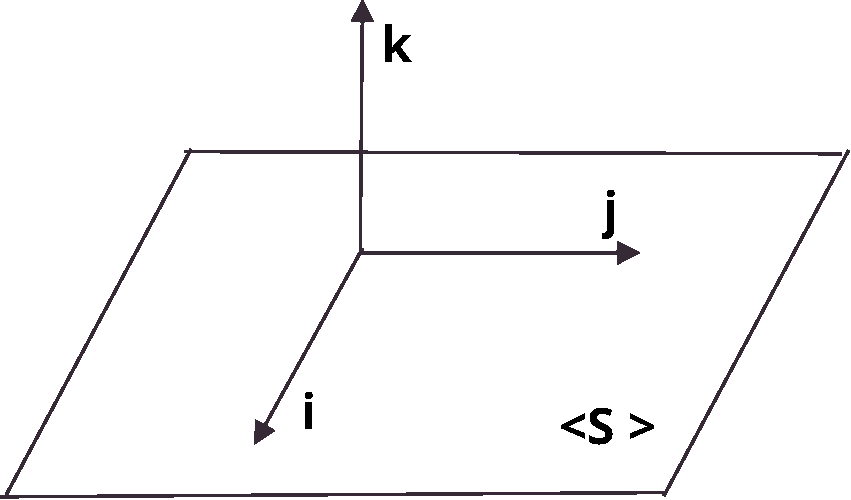
\includegraphics[width=6cm]{image/lecture-1.pdf} $\widetilde{s} = \{i+j\}$ 
    \end{enumerate}
  \end{example}
  \begin{definition}
    Если $V=\langle S \rangle$, то $S$ называется порождающим множеством векторного простанства $V$. Говорят, что векторное пространство $V$ порождается множеством $S$. 
  \end{definition} 
  \begin{definition}
    Если $\exists$ конечное множество $S$, т.ч. $V=\langle S \rangle$, то $V$ называется конечномерным (конечнопорожденным), иначе - бесконечномерным.
  \end{definition} 
  \begin{example1}
    $\R^n = \langle (1,0,...,0),...,(0,...,0,1) \rangle$ 
  \end{example1}
\begin{lemma} (Переформулировка ОЛЛЗ)
  Пусть векторное пространство $V$ пораждается $k$ векторами. Тогда любые $m>k$ векторов из $V$ - ЛЗ.
\end{lemma} 
\subsection{Базис}
$V$- конечномерное векторное простанство над $\R$ 
\begin{definition}\tab[-0.1cm]\textbf{1} 
  Система векторов $\{e_1,...,e_n\}\subseteq V$ называется базисом векторного пространства $V$, если:
  \begin{enumerate}
    \item $\{e_1,...,e_n\}$ - ЛНЗ
    \item $V = \langle e_1,...,e_n \rangle$, т.е. $\forall x \in V, \tab[0.1cm] \exists \tab[0.1cm] x_1,...,x_n \in \R: x = x_1e_1+\cdots + x_ne_n$  
  \end{enumerate}
  Эти числа $x_1,...,x_n$ - называются координатами вектора $x$ в базисе $\{e_1,...,e_n\}$ 
\end{definition} 
\begin{definition}\tab[-0.1cm]\textbf{2} 
  Система векторов $\{e_1,...,e_n\} \subseteq V$ называется базисом векторного простанства $V$, если любой вектор $x \in V$ выражается через $\{e_1,...,e_n\}$ единственным образом.
\end{definition} 
  \begin{subtheorem}
    (\textbf{Опр 1}) $\Longleftrightarrow $ (\textbf{Опр 2})
  \end{subtheorem} 
  \begin{proof}
    По лемме \eqref{lem3}.
  \end{proof}
  \begin{theorem}
    Всякое конечномерное векторное пространство над $\R$ обладает базисом. Более того, из любого конечного порожденного множества можно выбрать базис.
  \end{theorem} 
  \begin{proof}
    Пусть $S$ - какое-то порождающее множество векторного пространства $V$. \\
    Если $S$ - ЛНЗ, то $S$ - базис \\
    Если $S$ - ЛЗ, то по критерию о ЛЗ один из векторов $S_1$ множества $S$ линейно выражается через остальные. \\
    Тогда $S_1$ = $S\setminus\{s_1\}$ - конечное порождащее множество. ч.т.д. \\
    Т.к. $S$ - конечное,то этот процесс прервется и мы получим ЛНЗ порожденную систему.
  \end{proof} 
  \begin{theorem}
    В любом базисе конечномерного векторного пространства $V$ над $\R$ одно и тоже число векторов.
  \end{theorem} 
  \begin{proof}
    Пусть есть два базиса $\{e_1,...,e_n\}$ и $\{f_1,...,f_m\}$ векторного пространства $V$. 
    Тогда каждый вектор $f_i$ выражается через $e_1,...,e_n$. \\
    По ОЛЛЗ: $\{f_1,...,f_m\}$ - ЛЗ $\Longrightarrow \{f_1,...,f_m\}$ - не базис $\Longrightarrow $ противоречие.  
  \end{proof} 
  \begin{definition}
    Число векторов в базисе конечномерного векторного пространства $V$ называется размерностью векторного простанства и обозначается: $\dim V$ 
  \end{definition} 
  \begin{example} $\tab$ 
    \begin{enumerate}
      \item $\dim V^2 = 2$
      \item $\dim \R^n = n$   
    \end{enumerate}
  \end{example}
  \begin{remark}
    Если $V={0}$, то $\dim V = 0$ (базис систоит из $\varnothing$ ) 
  \end{remark} 
   Пусть $V$- векторное пространство над $\R$, $\dim V=n,\tab[0.1cm] S\subseteq V$ Любые $m>n$ векторов в $S$ - ЛЗ. (из ОЛЛЗ) \\
   $\Longrightarrow $ в $S \ \exists $ максимальная ЛНЗ подсистема (т.е. ничего нельзя добавить к этой подсистеме без нарушения ЛНЗ) 
  \begin{lemmanum} \label{lem6}
    Пусть $V$ - n-мерное векторное пространство над $\R,\tab[0.1cm] S\subseteq V$. Тогда максимальная ЛНЗ система векторов из $S$ образует базис в лин. оболочке $\langle S \rangle$  
  \end{lemmanum} 
  \begin{proof}
    Пусть $\{s_1,...,s_k\}$ максимальная (по включению) ЛНЗ система в $S$ $\Longrightarrow \forall s \in S \setminus \{s_1,...,s_k\}\Longrightarrow \{s,s_1,...,s_k\} - \text{ЛЗ.} $ \\
    По Лемме \eqref{lem2}. $\Longrightarrow s=\lambda_1s_1+\cdots+\lambda_ks_k$ \\
    Докажем, что $\{s_1,...,s_k\}$ - базис в $\langle S \rangle$. 
    \begin{enumerate}
      \item ЛНЗ (очевидно)
      \item $\forall x \in \langle S \rangle\tab[-0.1cm]: x = x_1s_1+\cdots+x_ks_k$ 
    \end{enumerate}
    По определению линейной оболочки $x$ линейно выражается через вектора из $S$ \\
    А каждый вектор из $S$ линейно выражается через $\{s_1,...,s_k\}$ 
  \end{proof}
  \begin{theorem}
    Пусть $V$ конечномерное векторное пространство над $\R$, тогда:
    \begin{enumerate}
      \item Любая максимальная ЛНЗ система векторов из $V$ - базис $V$.
      \item Любую ЛНЗ систему векторов из $V$ можно дополнить до базиса векторного пространства $V$. 
    \end{enumerate}
  \end{theorem}  
  \begin{proof} $\tab$ 
    \begin{enumerate}
      \item По лемме \eqref{lem6}. $S=V$ 
      \item Пусть $S$ - ЛНЗ система векторов из $V$ 
    \end{enumerate}
    Если $V=\langle S \rangle$, тогда $S$- базис. \\
    Если $V \neq \langle S \rangle$ , то $\exists s_1 \in V \setminus \langle S \rangle$ \\
    $\Longrightarrow s_1$ линейно не выражается через $S$ $\Longrightarrow \text{(По лемме \ref{lem2}.) } S_1=S \cup \{s_1\}$ - ЛНЗ. \\
    $\Longrightarrow $ Если $V = \langle S_1 \rangle$, то $S_1$ базис, иначе $\exists S_2 \in V \setminus \langle S_1 \rangle$, и т.д. \\
    Этот процесс прервется на конечном шаге, т.к. пространство $V$- конечное. (Если $\dim V \neq n, \text{то} \not\exists$ ЛНЗ системы с числом векторов $> n$) 
  \end{proof} 
  \begin{consequense} 
    Пусть $V$ конечномерное векторное пространство над $\R$ 
    \begin{enumerate}
      \item Любой ненулевой вектор можно дополнить до базиса.
      \item Любые $n$ ЛНЗ вектора в $n$-мерном пространстве $V$ образуют базис.
    \end{enumerate}
  \end{consequense} 
  
  \section{Ранг}
  \subsection{Ранг системы векторного простанства}
  \begin{definition}
    Рангом системы векторов $S$, назовем $\\dim \langle S \rangle$, т.е. число векторов в максимальной ЛНЗ системе из $S$.  
  \end{definition} 
  $A$ - матрица $m \times n$ \\ $\\$
  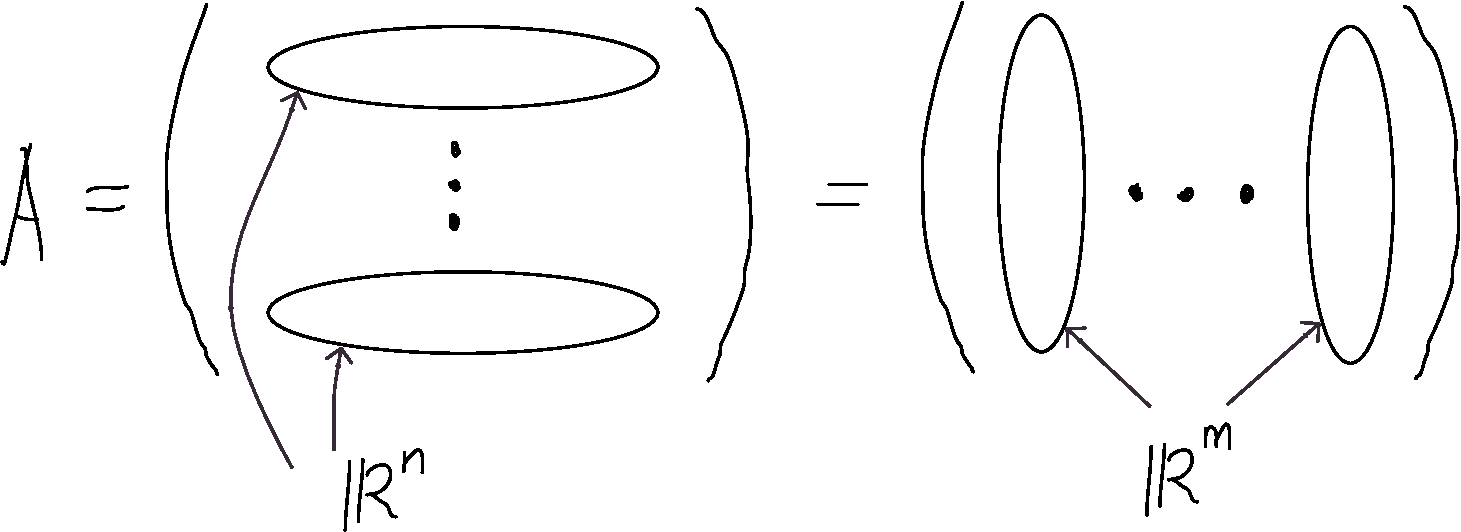
\includegraphics[width=15cm]{image/lecture-2.pdf}
  \begin{definition}
    Рангом матрицы $A$ называется ранг системы ее строк, т.е. максимальное число ЛНЗ строк матрицы.
  \end{definition} 
  \subsection{Ранг матрицы}
  \begin{definition}
    Ранг системы векторов $\{s_1,...,s_n\}$ называется $\dim \langle s_1,...,s_n \rangle$.
  \end{definition} 
  \begin{definition}
    Рангом матрицы $A \ m\times n$ называется ранг системы её строк. $$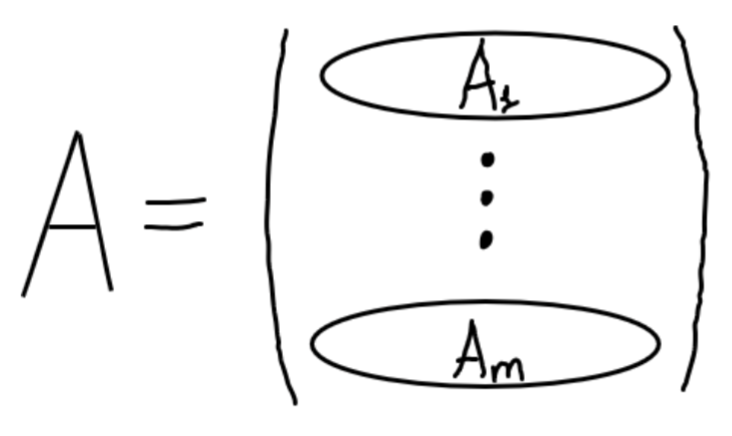
\includegraphics[width=4cm]{image/lecture-3.png}$$
  \end{definition} 
  \begin{definition}
    Две системы векторов $\{v_1,...,v_n\}$, $\{w_1,...,w_n\}$ называются эквивалентными, если каждый вектор $v_i$ линейно выражается через $\{w_1,...,w_n\}$, а $w_i$ через $\{v_1,...,v_n\}$. \\
    Это условная эквивалентность: $\langle v_1,...,v_n \rangle = \langle w_1,....,w_n \rangle$ 
  \end{definition} 
  \begin{subtheorem}
    При элементарных преобразованиях над строками ранг матрицы $A$  не изменяется.
  \end{subtheorem} 
  \begin{proof} 
    $$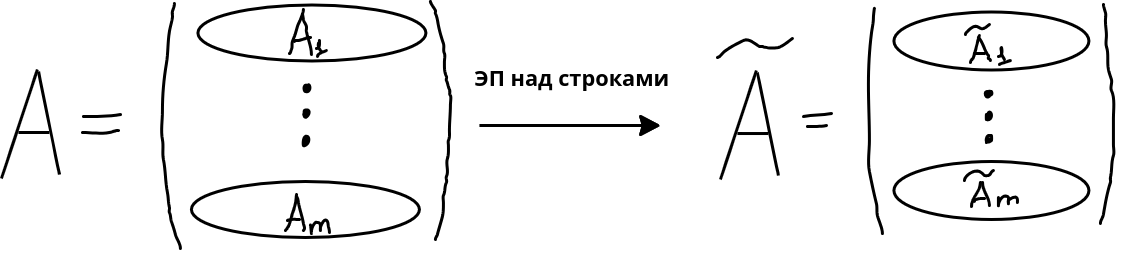
\includegraphics[width=12cm]{image/lecture-4.png}$$
    $$\langle A_1,...,A_m \rangle = \langle \widetilde{A_1},...,\widetilde{A_m} \rangle$$ \\
    т.е. система строк $A$ эквивалентна системе строк $\widetilde{A}$ $\Longrightarrow rkA = rk \widetilde{A}$. 
  \end{proof} 
  \begin{subtheorem}
    При элементарных преобразованиях над столбцами, ранг матрицы $A$  не изменяется.
  \end{subtheorem} 
  \begin{offernum}
    Ранг матрицы $A$ равен числу ненулевых строк матрицы ступенчатого вида, к которому можно привести матрицу $A$ с помощью элементарных преобразований строк.
  \end{offernum} 
  \begin{proof}
    $A \overset{\text{ЭП строк}}{\longrightarrow } A_{\text{ст}} \Longrightarrow  rkA = rkA_{\text{ст}}$ \\
    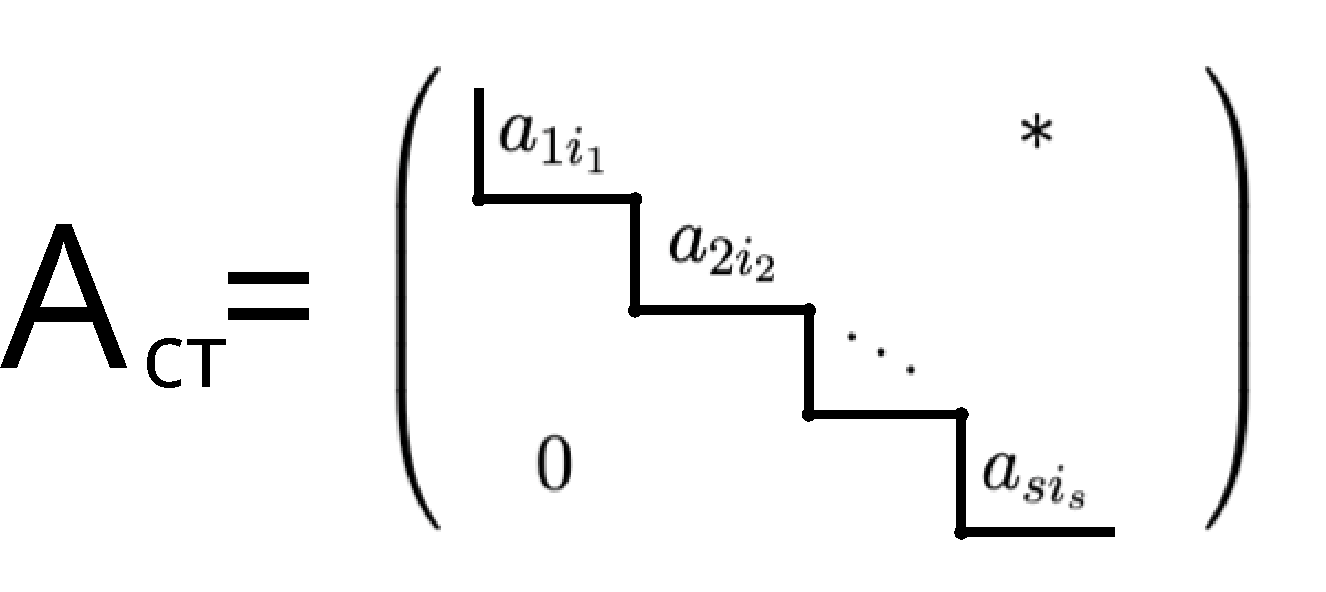
\includegraphics[width=5cm]{image/lecture-5.pdf}
    $a_{1i_1},...,a_{si_s}$ - лидеры строк в $A_{\text{ст}} \Longrightarrow a_{1i_1} \neq 0,...,a_{si_s} \neq 0$ \\
    Очевидно, что $rkA_{\text{ст}}\leq s$. Достаточно доказать, что ненулевые строки ЛНЗ. 
    Рассмотрим ЛК: \\
    $\lambda_1(0,...,0,a_{1i_1},\ast,...,\ast) + \lambda_2(0,...,0,a_{2i_2},\ast,...,\ast) + \cdots + \lambda_s(0,...,0,a_{si_s},\ast,...,\ast) = (0,...,0)$ \\
    $(0,...,0,\lambda_1 a_{1i_1},...,\lambda_1a_{1i_2} + \lambda_2a_{2i_2},...) = (0,...,0) \Longrightarrow \lambda_1 \underbrace {a_{1i_1}}_{\text{лидер}}= 0 \Longrightarrow \lambda_1 = 0$ \\
    $\lambda_1a_{i_21} + \lambda_2\underbrace {a_{2i_2}}_{\text{лидер}} = 0 \Longrightarrow \lambda_2 = 0$ и т.д. \\
    Получаем, что $\lambda_1 = 0,...,\lambda_s = 0 \Longrightarrow$ это ЛК - ЛНЗ. 
  \end{proof} 
  \begin{offernum}
    Ранг системы столбцов не изменяется при элементарных преобразованиях над строками.
  \end{offernum}
  \begin{proof} 
    $$A \overset{\text{ЭП строк}}{\longmapsto}\widetilde{A}$$ \vspace{0.35cm} 
    Пусть $A = (a_{ij}) = (\underbrace{A_1,...,A_n}_{\text{столбцы }A})$, $\widetilde{A} = (\widetilde{a_{ij}}) = (\underbrace{\widetilde{A_1},...,\widetilde{A_n}}_{\text{столбцы }\widetilde{A}})$. \vspace{0.3cm} \\
    Докажем, что если для некоторых чисел $\lambda_1,...,\lambda_n \in \R$ выполнено:\\ $\lambda_{1}A_1 + \cdots + \lambda_nA_n = 0$, то для этих же чисел  $\lambda_1 \widetilde{A_1} + \cdots + \lambda_n \widetilde{A_n} = 0$ 
    (Верно и обратное, т.к. ЭП обратимы, т.е. если для каких-то чисел $\lambda_i \in \R: \sum \lambda_i \widetilde{A_1} = 0$, то $\sum \lambda_i A_i = 0$). \\
    Дано: $\lambda_1A_1 + \cdots + \lambda_nA_n = \begin{pmatrix}
      0\\
      \vdots\\
      0
    \end{pmatrix}\Longrightarrow$ 
    $\begin{cases}
      \lambda_1a_{11} + \lambda_2a_{12} + \cdots + \lambda_na_{1n} = 0 \\
      \vdots \\
      \lambda_1a_{m1} + \lambda_2a_{m2} + \cdots + \lambda_na_{mn} = 0
    \end{cases}$ 
    $\Longrightarrow \vspace{0.3cm} \\  \lambda_1,...,\lambda_n - \text{решение ОСЛУ } AX=0$. 
    Т.к. при ЭП над уравнениями множество решений не меняется, поэтому $\lambda_1,...,\lambda_n$ - это решение ОСЛУ $\widetilde{A}X=0$
    $\Longrightarrow \lambda_1 \widetilde{A_1} + \cdots + \lambda_n \widetilde{A_n} = 0$ \\
    Отсюда получаем, что если $A_{i_1},...,A_{i_s}$ - максимальная ЛНЗ система столбцов в $A$, то $\widetilde{A_{i_1}},...,\widetilde{A_{i_s}}$ - максимальная ЛНЗ система столбцов в $\widetilde{A}$ $\Longrightarrow rk\{\widetilde{A_1},...,\widetilde{A_n}\} = rk\{A_1,...,A_n\}.$ 
  \end{proof} 
  \begin{definition}
    Пусть $A = (a_{ij})$ - матрица $m\times n $, тогда $B = (b_{ij}) \text{ матрица } n\times m$ называется транспонированной к матрице $A$, если $b_{ij} = a_{ji}$, где $i = \overline{1,m}; j = \overline{1,n}$ \\
    Обозначаем $B = A^T$  
  \end{definition} 
  \begin{example1}
    $$\begin{pmatrix}
      1&2&3\\
      4&5&6
    \end{pmatrix}^T
    = \begin{pmatrix}
      1&4\\
      2&5\\
      3&6
    \end{pmatrix}$$ 
  \end{example1}
  \begin{consequense} 
    Ранг системы строк матрицы $A$ (=рангу матрицы $A$) не изменяется при элементарных преобразованиях над столбцами. 
  \end{consequense} 
  \begin{proof}
    Предложение 2 применяем к $A^T$ 
  \end{proof} 
  \begin{theoremnum} 
    Ранг системы строк матрицы $A$ совпадает с рангом системы столбцов матрицы $A$.
  \end{theoremnum} 
  \begin{proof}
    Было доказано, что ранг системы строк (столбцов) матрицы не изменяется при ЭП над строками и над столбцами. Приведем матрицу $A$ к ступенчатому виду с помощью ЭП над строками. $A_\text{ст}$ имеет вид:
    $$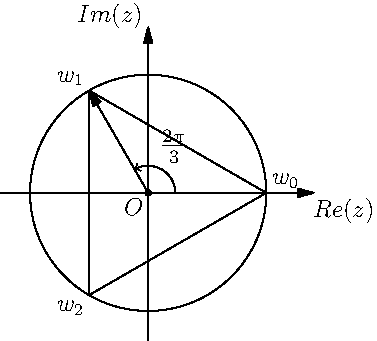
\includegraphics[width=5cm]{image/lecture-6.pdf}$$
    $$a_{1i_1} \neq 0,...,a_{si_s} \neq 0$$ 
    Используем $i_1$-столбец, вычитая этот столбец из оставшихся с подходящими коэффициентами, получаем:
    $$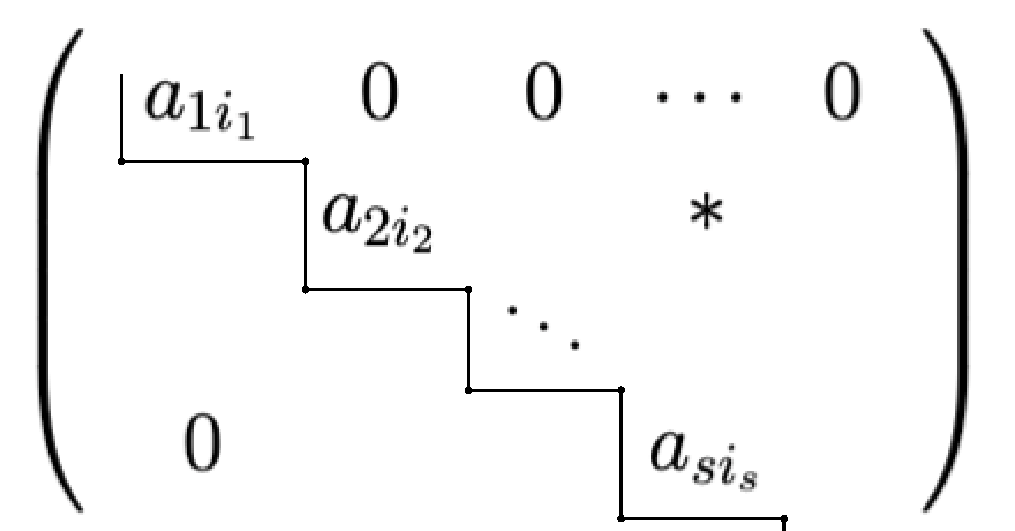
\includegraphics[width=5cm]{image/lecture-7.pdf}$$ 
    Далее используем $i_2$-столбец, обнуляем все элементы правее $a_{i_22}$. В итоге получаем: $$\begin{pmatrix}
      a_{1i_1} && \null && 0\\
      \null && \ddots && \null\\
      0 && \null && a_{si_s}
    \end{pmatrix}$$
    Очев, что у такой матрицы ранг системы строк = рангу системы столбцов.
  \end{proof} 
  \section{Возвращаемся к системе линейных уравнений}
  $\begin{cases}
    a_{11}x_1 + ... + a_{1n}x_n = b_1 \\ 
    a_{21}x_2 + ... + a_{2n}x_n = b_2 \\
    \vdots \\
    a_{m1}x_1 + ... + a_{mn}x_n = b_m
  \end{cases} (AX = B)$
  \begin{theorem} (Кронекера-Капелли)
    \begin{enumerate}
      \item (Критерий совместимости СЛУ) \\ CЛУ $AX = B$ совместна $\Longleftrightarrow rk(A|B) = rkA$ 
      \item (Критерий определенности СЛУ) \\ Совместная СЛУ $AX =B$ - определена $\Longleftrightarrow rk(A|B) = rkA = n$ 
      \item (Критерий существования нетривиального решения у однородной СЛУ) \\ ОСЛУ $AX = 0$ имеет нетривиальное решение $\Longleftrightarrow rkA<n$ 
    \end{enumerate}
  \end{theorem}
  \textbf{Однородная СЛУ} \\  
  $\begin{cases}
    a_{11}x_1 + ... + a_{1n}x_n = 0 \\ 
    a_{21}x_1 + ... + a_{2n}x_n = 0 \\
    \vdots \\
    a_{m1}x_1 + ... + a_{mn}x_n = 0
  \end{cases} (AX = 0)$
  \begin{subtheorem}
    ОСЛУ всегда совместна, т.к. есть тривиальное решение.
  \end{subtheorem} 
  \begin{properties} $\tab$ 
    \begin{enumerate}
      \item Если $X^0$ = $\begin{pmatrix}
        x_1^0\\
        \vdots\\
        x_n^0 
      \end{pmatrix}$; \tab[0.3cm] $\widetilde{X^0}$ = $\begin{pmatrix}
        \widetilde{x_1^0}\\
        \vdots\\
        \widetilde{x_n^0} 
      \end{pmatrix}$ - решение ОСЛУ, \\ \tab[9cm] тогда $X^0 + \widetilde{X^0}$ = $\begin{pmatrix}
        X_1^0 + \widetilde{X_1^0} \\
        \vdots\\
        X_n^0 + \widetilde{X_n^0}
      \end{pmatrix}$
      \item Если $X^0$ = $\begin{pmatrix}
        x_1^0\\
        \vdots\\
        x_n^0 
      \end{pmatrix}$ - решение ОСЛУ $AX = 0$, то $\lambda X^0$ = $\begin{pmatrix}
        \lambda x_1^0\\
        \vdots\\
        \lambda x_n^0 
      \end{pmatrix}$ - решение.
    \end{enumerate}
  \end{properties}
  \begin{proof}
    Д/з
  \end{proof} 
  \begin{consequense}
    Множество всех решений ОСЛУ является векторным \\ подпространством в $\R^n$. Будем говорить, что это пространство над ОСЛУ.
  \end{consequense} 
  \begin{remark}
    Если $\exists$ нетривиальное решение ОСЛУ над $\R$, то $\exists$ бесконечно много решений.
  \end{remark} 
  \begin{theoremnum}
    Пространство решений ОСЛУ $AX = 0$ имеет базис из $n-r$ векторов, где $n$ - число неизвестных, а $r=rkA$.
  \end{theoremnum} 
  \subsection{Фундаментальная система решений}
  \begin{definition}
    Любой базис пространства решений ОСЛУ называется \\ Фундаментальной Системой Решений ОСЛУ (ФСР).
  \end{definition} 
  \begin{proof}
    (Теоремы 2.) \\ Решение СЛУ методом Гаусса: приводим её к ступенчатому виду (число ступенек $r=rkA$), главные неизвестные выражаем через свободные. 
    $$\begin{cases}
      x_1=c_{1,1}x_{r+1} + \cdots + c_{1,n-r}x_n \\
      \vdots\\
      x_r=c_{r,1}x_{r+1} + \cdots + c_{r,n-r}x_n
    \end{cases}$$ 
    Определим $n-r$ частных решений, приравнивая одно из $x_1,...,x_n$ к 1, а остальные к 0. 
    $$F_1 = \begin{pmatrix}
      c_{11}\\
      \vdots\\
      c_{r1}\\
      \hline
      1\\
      0\\
      \vdots\\
      0
    \end{pmatrix}, \ \ F_2 = \begin{pmatrix}
      c_{12}\\
      \vdots\\
      c_{r2}\\
      \hline
      0\\
      1\\
      \vdots\\
      0
    \end{pmatrix} \ ,..., \ F_{n-r} = \begin{pmatrix}
      c_{1,{n-r}}\\
      \vdots\\
      c_{r,{n-r}}\\
      \hline
      0\\
      0\\
      \vdots\\
      1
    \end{pmatrix}$$  
    Докажем, что $F_1,...,F_{n-r}$ - базис пространства решений ОСЛУ 
    \begin{enumerate}
      \item $F_1,...,F_{n-r}$ - ЛНЗ? \\
      Рассмотрим ЛК $\lambda_1F_1 + \cdots + \lambda_{n-r}F_{n-r} = \begin{pmatrix}
        0 \\ \vdots \\ 0
      \end{pmatrix} \\ \Longrightarrow \begin{pmatrix}
        \ast \\ \vdots \\ \ast \\ \hline \lambda_1 \\ \vdots \\ \lambda_{n-r}
      \end{pmatrix} = \begin{pmatrix}
        0 \\ \vdots \\ 0
      \end{pmatrix} \Longrightarrow \lambda_1 = 0,...,\lambda_{n-r}=0$ 
      \item Надо доказать, что любое решение выражено через $F_1,...,F_{n-r}$ \\ $\\$ 
      $X^0 = \begin{pmatrix}
        c_{11} \\ \vdots \\ c_{r1} \\ \hline \mu_{r+1} \\ \vdots \\ \mu_n
      \end{pmatrix} = \mu_{r+1}F_1 + \cdots + \mu_nF_{n-r}$ 
    \end{enumerate}
  \end{proof}
  \begin{example1} Найти ФСР ОСЛУ \end{example1} 
  $\begin{cases}
    x_1 + x_2 + 3x_3+5x_4-x_5 = 0\\
    x_1 + 2x_2 + x_3 + x_4 + x_5 = 0
  \end{cases}$ 
  $$\begin{pmatrix}
    1 & 1 & 3 & 5 & -1 \\
    1 & 2 & 1 & 1 & 1
  \end{pmatrix}\rightarrow 
  \begin{pmatrix}
    1 & 1 & 3 & 5 & -1 \\
    0 & 1 & -2 & -4 & 2 
  \end{pmatrix} \rightarrow
  \begin{pmatrix}
    1 & 0 & 5 & 9 & -3 \\
    0 & 1 & -2 & -4 & 2
  \end{pmatrix}$$
  где $x_1, x_2$ - главные, $x_3, x_4, x_5$ - свободные \\ $\\$ 
  $\begin{cases}
    x_1 = -5x_3 - 9x_4 +3x_5 \\
    x_2 = 2x_3+4x_4-2x_5
  \end{cases}$ $x_3, x_4, x_5 \in \R$ - произвольные 
  $$F_1 = \begin{pmatrix}
    -5 \\ 2 \\ \hline 1 \\ 0 \\ 0
  \end{pmatrix}, \tab[0.5cm] F_2 = \begin{pmatrix}
    -9 \\ 4 \\ \hline 0 \\ 1 \\ 0
  \end{pmatrix}, \tab[0.5cm] F_3 = \begin{pmatrix}
    3 \\ -3 \\ \hline 0 \\ 0 \\ 1
  \end{pmatrix} \tab[0.1cm] \text{ - три частных решения ОСЛУ}$$ 
  Проверим, что $\{F_1,F_2, F_3\}$- базис пространства решений ОСЛУ \\ $\\$ 
  $\begin{pmatrix}
    * \\ * \\ \hline \lambda_1 \\ \lambda_2 \\ \lambda_3
  \end{pmatrix} = 
  \lambda_1F_1 + \lambda_2F_2 + \lambda_3F_3 = \begin{pmatrix}
    0 \\ 0 \\ 0 \\ 0 \\ 0
  \end{pmatrix} \Longrightarrow \lambda_{1,2,3} = 0 \Longrightarrow F_1, F_2, F_3$ - ЛНЗ. \\ $\\$ 
  Проверим, что $\{F_1,F_2, F_3\}$ порождает пространство решений. Возьмем произвольные числа $\mu_3, \mu_4, \mu_5$ и приравняем $x_3 = \mu_3, x_4 = \mu_4, x_5 = \mu_5$  
  $$\begin{pmatrix}
    x_1 \\ x_2 \\ \hline x_3 \\ x_4 \\ x_5
  \end{pmatrix} = \begin{pmatrix}
    -5\mu_3-9\mu_4+3\mu_5 \\ 2\mu_3 + 4\mu_4-2\mu_5 \\ \hline \mu_3 \\ \mu_4 \\ \mu_5
  \end{pmatrix} = \mu_3 \begin{pmatrix}
    -5 \\ 2 \\ \hline 1 \\ 0 \\ 0
  \end{pmatrix} + \mu_4 \begin{pmatrix}
    -9 \\ 4 \\ \hline 0 \\ 1 \\ 0
  \end{pmatrix} + \mu_5 \begin{pmatrix}
    3 \\ -2 \\ \hline 0 \\ 0 \\ 1 
  \end{pmatrix}$$ 
  Такой базис называется нормальной ФСР. 
  \subsection{Неоднородная СЛУ}
  $\begin{cases}
    a_{11}x_1 + ... + a_{1n}x_n = b_1 \\ 
    a_{21}x_2 + ... + a_{2n}x_n = b_2 \\
    \vdots \\
    a_{m1}x_1 + ... + a_{mn}x_n = b_m
  \end{cases} (AX=B)$ \\ $\\$ 
  Рассмотрим соответствующую (ассоциированную) к ней ОСЛУ \\ $\\$ 
  $\begin{cases}
    a_{11}x_1 + ... + a_{1n}x_n = 0 \\ 
    a_{21}x_2 + ... + a_{2n}x_n = 0 \\
    \vdots \\
    a_{m1}x_1 + ... + a_{mn}x_n = 0
  \end{cases} (AX=0)$ 
  \begin{theorem}
    Пусть СЛУ $AX=B$ - совместна. $X_0$ - произвольное частное решение. Тогда множество $M$ всех решений неоднородной СЛУ: $AX=B$ равно сумме частного решения $X_0$ и множеству $M_{\text{одн}}$ всех решений соответствующей однородной СЛУ: $AX=0$ 
    $$M = X_0 + M_{\text{одн}} = \{X_0 + Y | Y \in M_{\text{одн}}\}$$ 
  \end{theorem}
  \begin{proof}
    $X_0 + M_{\text{одн}} \subseteq M$ \\
    Рассмотрим произвольное решение ОСЛУ. $Y \in M_{\text{одн}}$ \\ $\\$ 
    Пусть $X_0 = \begin{pmatrix}
      x_1^0 \\ \vdots \\ x_n^0
    \end{pmatrix}, \tab[0.2cm] Y = \begin{pmatrix}
      y_1 \\ \vdots \\ y_n
    \end{pmatrix}$ \\
    \tab[1.8cm]Докажем, что $X_0 + Y = \begin{pmatrix}
      x_1^0 + y_1 \\ \vdots \\ x_n^0 + y_n
    \end{pmatrix}$ - решение СЛУ, т.е. $X_0 + Y \in M$ 
    $$AX=B: \  a_{i1}x_1^0 + \cdots + a_{in}x_n^0 = b_i$$
    $$AX=0: \ a_{i1}y_1 + \cdots + a_{in}y_n = 0$$
    где $i = \overline{1,m}$. \\
    Проверим, что $X_0 + Y \in M$ 
    $$a_{i1}(x_1^0 + y_1) + \cdots + a_{in}(x_n^0 + y_n) = b_i$$
    $$(\underbrace{a_{i1}x_1^0 + \cdots + a_{in}x_n^0}_{b_i \text{ (т.к. } X_0 \in M)}) + (\underbrace{a_{i1}y_1 + \cdots + a_{in}y_n}_{0 \text{ (т.к. } Y \in M_{\text{одн}})}) = b_i$$  
    Обратное утверждение:
    $M \subseteq X_0 + M_{\text{одн}}$ \\
    Рассмотрим произвольное решение $Z = \begin{pmatrix}
      z_1 \\ \vdots \\ z_n 
    \end{pmatrix}$ - неоднородная СЛУ. \\
    Докажем, что $Z - X_0 = \begin{pmatrix}
      z_1 - x_1^0 \\ \vdots \\ z_n - x_n^0
    \end{pmatrix}
    $ - решение однородной СЛУ. \\
    Проверяем
    $$a_{i1}(z_1 - x_1^0) + \cdots + a_{in}(z_n - x_n^0) = 0$$ 
    $$(\underbrace{a_{i1}z_1 + \cdots + a_{in}z_n}_{b_i (\text{т.к. } Z \in M)}) - (\underbrace{a_{i1}x_1^0 + \cdots + a_{in}x_n^0}_{b_i (\text{т.к. } X_0 \in M)}) = 0$$ 
  \end{proof}  
  \begin{remark} $\\$ 
    Общее решение ОСЛУ имеет вид: $$X = \mu_1F_1 + \cdots + \mu_sF_s$$где $F_1,...,F_s$ - ФСР ОСЛУ, $s = n - rkA$  \\
    Общее решение неоднородной СЛУ: $$X = X_0 + \mu_1F_1 + \cdots + \mu_sF_s$$ $X_0$ - частное решение неоднородной СЛУ
  \end{remark} 
  \section{Операции над матрицами}
  $Mat_{m \times n}(\R)$ - множество всех матриц размера $m \times n$ с коэффициентами из $\R$ \\
  $A, B \in Mat_{m \times n}(\R), \ A=(a_{ij}), \ B=(b_{ij})$ 
  \begin{enumerate}
    \item Сложение матриц \\
    Суммой матриц $A$ и $B$ называется матрица $C=(c_{ij})$ размера $m \times n$, у которой $c_{ij} = a_{ij} + b_{ij}$. Обозначается: $C = A + B$
    \item Умножение матриц на число $\lambda \in \R$ \\ Произведением матрицы $A=(a_{ij})$ на $\lambda$ называется матрица $C=(c_{ij})$ размера $m \times n$, у которой $c_{ij} = \lambda a_{ij}$. Обозначается: $C = \lambda A$
    \begin{subtheorem}
      Множество $Mat_{m \times n}(\R)$, относительно этих операций сложения и умножения на число, образует векторное пространство над $\R$. 
    \end{subtheorem} 
    \begin{proof}
      $A,\tab [0.2cm]B \in Mat_{m \times n}(\R) \Longrightarrow A+B, \tab [0.2cm]\lambda A \in Mat_{m \times n}(\R)$ \\
      Надо проверить 8 аксиом
      \begin{itemize}
        \item[1)] коммутативность \\
        $C = A + B \tab[0.5cm] c_{ij} = a_{ij} + b_{ij}$ \\
        $\widetilde{C} = B + A \tab[0.5cm] \widetilde{c_{ij}} = b_{ij} + a_{ij}$ \\
        т.к. сложение вещественных чисел из $\R$ - коммутативно, то $c_{ij} = \widetilde{c_{ij}} \Longrightarrow C = \widetilde{C}$ \\
        $\Longrightarrow A + B = B + A$
        \begin{Exercise} Аналогично доказать 2), 5)-8)\end{Exercise}
        \item[3)] $\exists 0 \in Mat_{m \times n}(\R)$
        $\forall A \in Mat_{m \times n}(\R): 0 + A = A$ \\
        В качестве 0 берем нулевую матрицу размера $m \times n$
        \item[4)] $\forall A \in Mat_{m \times n}(\R) \ \exists B \in Mat_{m \times n}(\R): A+B=0$ \\В качестве $B$ берем $b_{ij} = -a_{ij}$ 
      \end{itemize}
    \end{proof} 
    \begin{subtheorem}
      $\dim M_{m \times n} = m \cdot n$
    \end{subtheorem} 
    \begin{proof}
      Достаточно указать базис \\ 
      $\{E_{st}\}$, $s = \overline{1,m}, \ t = \overline{1,n}$ \\
      $E_{st} = (a_{ij})$, $a_{ij} = \begin{cases}
        1, \ i=s, \ j=t \\ 0 \text{, иначе}
      \end{cases}$
      \begin{Exercise}
        Проверить, что это базис.
      \end{Exercise}
    \end{proof} 
    \begin{definition}
      Матрица $E_{st}$ называется матричной единицей. Базис из всех матричных единиц называется стандартным базисом в пространстве $Mat_{m \times n}(\R)$. $A = \sum a_{st} E_{st}$ 
    \end{definition} 
    \item Умножение матриц \\
    $A \in Mat_{m \times k}(\R), \tab[0.2cm]B \in Mat_{k \times n}(\R)$ \\
    Произведение матрицы $A$ на матрицу $B$ называется матрица $C$ размера $m \times n$, у которой $c_{ij} = \sum \limits_{s=1}^{k}a_{is}b_{sj}$. Обозначаем $C = AB$.
    \begin{properties1}
      Произведение матриц не коммутативно.
    \end{properties1}
    \begin{example1}
      $$A = \begin{pmatrix}
        1 & 0 \\ 0 & 0
      \end{pmatrix}, \tab[0.3cm] B = \begin{pmatrix}
        0 & 1 \\ 0 & 0
      \end{pmatrix}$$
      $$AB = \begin{pmatrix}
        0 & 1 \\ 0 & 0
      \end{pmatrix}, \tab[0.3cm] BA = \begin{pmatrix}
        0 & 0 \\ 0 & 0
      \end{pmatrix} \Longrightarrow AB \neq BA$$ 
    \end{example1}
    \begin{remark} $\\ \\$
      $\begin{cases}
        a_{11}x_1 + \cdots + a_{1n}x_n = b_1 \\
        \vdots \\
        a_{m1}x_1 + \cdots + a_{mn}x_n = b_n
      \end{cases} \Longleftrightarrow \begin{pmatrix}
        a_{11} & \cdots & a_{1n} \\
        \vdots & \null & \vdots \\
        a_{m1} & \cdots & a_{mn}
      \end{pmatrix} \begin{pmatrix}
        x_1 \\ \vdots \\ x_n
      \end{pmatrix} = \begin{pmatrix}
        b_1 \\ \vdots \\ b_m
      \end{pmatrix}$
    \end{remark} 
  \end{enumerate}
  \begin{example}\end{example}
    \begin{enumerate}
      \item Проекция \\
      $\phi: V^3 \to V^2, \phi: x_1i+x_2j+x_3k \to x_1i+x_2j$ 
      $$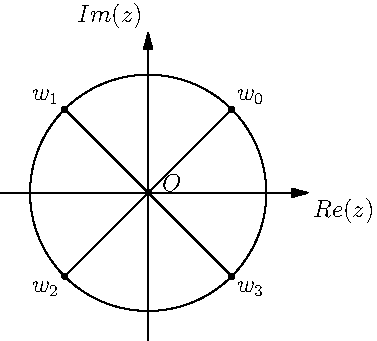
\includegraphics[width=6cm]{image/lecture-8.pdf}$$
      \item Поворот\\
      $\phi: V^2 \to V^2$ Поворот на угол $\alpha$ вокруг точки $O$ 
      $$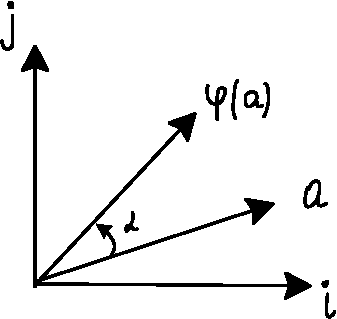
\includegraphics[width=3.5cm]{image/lecture-9.pdf}$$
    \end{enumerate}
    
  \section{Линейные отображения}
  \subsection{Изоморфизм}
  
  $V, W$- векторные пространства над $\R$ 
  \begin{definition}
    Отображение $\phi: V \to W$ называется изоморфизмом векторных пространств, если:
    \begin{enumerate}
      \item $\forall a, b \in V: \ \phi(a+b) = \phi(a) + \phi(b)$
      \item $\forall \lambda \in \R \ \forall a \in V: \ \phi(\lambda a) = \lambda \phi(a)$
      \item $\phi$ является биекцией. 
    \end{enumerate}
    При этом $V, W$ называются изоморфными. Обозначается $V \cong W$ 
  \end{definition} 
  \begin{subtheorem}
    Любое векторное  пространство над $\R$ размерности $n$ изоморфно $\R^n$. 
  \end{subtheorem} 
  \begin{proof}
    Фиксируем базис $\{e_1,...,e_n\}$ - в $V$.
    \begin{enumerate}
      \item $\forall x \in V$ однозначно раскладывается по базису $x = \sum \limits_{i=1}^{n} x_ie_i$. 
    Зададим отображение  $\phi: V \to \R^n$ по правилу:
    $$\phi: x = x_1e_1 + \cdots + x_ne_n \to (x_1,...,x_n)$$
    Т.к. координаты вектора определены однозначно, то $\phi$ инъективно, сюрьективность очевидна $\Longrightarrow $ $\phi$ - биекция.
    \item $\forall x,y \in V$
    $$x = \sum \limits_{i=1}^{n} x_ie_i \tab[0.5cm] y = \sum \limits_{i=1}^{n} y_ie_i \tab[0.5cm]
    x + y = \sum \limits_{i=1}^{n} (x_i + y_i)e_i$$ 
    $$\phi(x+y) = (x_1 + y_1,...,x_n+y_n) = (x_1,...,x_n) + (y_1,...,y_n) = \phi(x) + \phi(y)$$ 
    \item $\forall \lambda \in \R \tab[0.1cm] \forall x \in V$
    $$\phi(\lambda x) = \phi(\sum \limits_{i=1}^{n} \lambda x_ie_i) = (\lambda x_1,....,\lambda x_n) = \lambda (x_1,...,x_n) = \lambda \phi(x)$$  
    \end{enumerate}
  \end{proof} 

  \begin{example}\end{example}
  \begin{enumerate}
    \item $V^2 \cong \R^2 \\ V^3 \cong \R^3$ 
    \item $M_{m \times n}(\R) \cong \R^{mn}$
  \end{enumerate}
  \begin{Exercise}
    $V \cong W \Longleftrightarrow \dim V = \dim W; \tab[0.2cm] V,W - $ конечномерные пространства над $\R$.  
  \end{Exercise}
  \subsection{Линейные отображения и матрицы}
  \begin{definition}
    Отображение $\phi: V \to W$ называется линейным, если
    \begin{enumerate}
      \item $\forall a,b \in V \tab[0.3cm] \phi(a+b) = \phi(a) + \phi(b)$
      \item $\forall \lambda \in \R, \forall a \in V \tab[0.3cm] \phi(\lambda a) = \lambda \phi(a)$  
    \end{enumerate}
    
  \end{definition} 
  \begin{subtheorem}
    $V,W$- векторные пространства над $\R$. \\
      Если $\{e_1,...,e_n\}$ - базис $V$, ($w_1,...,w_n$) - набор векторов из $W$. \\Тогда $\exists$! линейное отображение $\phi: V \to W$, которое $\phi: e_i \to w_i \tab[0.3cm]\forall i = \overline{1,n}$.
  \end{subtheorem} 

  \begin{proof} \tab
    \begin{enumerate}
      \item Пусть $\phi: V \to W$ - линейное отображение такое, что \\$\phi(e_i) = w_i \tab[0.2cm] \forall i = \overline{1,n}$. Тогда образ вектора $x$ определяется однозначно по формуле: $$\phi(x) = \phi(x_1e_1 + \cdots + x_ne_n) = x_1 \phi(e_1) + \cdots + x_n \phi(e_n) = x_1 w_1 + \cdots + x_n w_n$$ где $x=x_1e_1 + \cdots + x_ne_n$ \\
      $\Longrightarrow$ линейное отображение определяется однозначно.
      \item Докажем, что $\exists$ линейное отображение, которое переводит $e_i$ в $w_i$. Отображение зададим формулой: $$\phi: x = x_1e_1 + \cdots + x_ne_n \to x_1w_1 + \cdots + x_nw_n$$
      $$\phi(a+b) = \phi((a_1+b_1)e_1 + \cdots + (a_n + b_n)e_n) = (a_1+b_1)w_1 + \cdots + (a_n + b_n)w_n$$
      $$\phi(a) + \phi(b) = \phi(a_1e_1 + \cdots a_ne_n) + \phi(b_1e_1 + \cdots b_ne_n) = $$ $$= a_1w_1 + \cdots + a_nw_n + b_1w_1 + \cdots + b_nw_n = w_1(a_1 + b_1) + \cdots + w_n(a_n + b_n)$$
      $\Longrightarrow \phi(a+b) = \phi(a) + \phi(b)$\\
      Проверить, что $\phi(\lambda a) = \lambda \phi(a)$ - ДЗ
    \end{enumerate}
  \end{proof} 
  Пусть $\phi: V \to W$ - линейное отображение $V$- $n$-мерное, $W - m$-мерное пространство.  \\
  Фиксируем базис 
  $\mathcal{E}  = \{e_1,...,e_n\}$ - базис в $V$; $\mathcal{F}  = \{f_1,...,f_m\}$ - базис в $W$
  $$\phi(e_1) = w_1 = a_{11}f_1 + \cdots + a_{m1}f_m$$ $$\vdots$$
  $$\phi(e_n) = w_n = a_{1n}f_1 + \cdots + a_{mn}f_m$$

  \begin{definition}
    Матрица $A$ размера $m \times n$,  составленая из столбцов координат образов векторов $e_i$ в образе $\mathcal{F}$, называется матрицей линейного отображения в базисах $\mathcal{E} $ и $\mathcal{F}$  
  \end{definition} 
  $$A = \begin{pmatrix}
    a_{11} & \cdots & a_{1n} \\
    \vdots & \null & \vdots \\
    \undermat{\phi(e_1)}{a_{m1}}  & \cdots & \undermat{\phi(e_n)}{a_{mn}} 
  \end{pmatrix}$$  
  \vspace{0.3cm}
  \begin{subtheorem}
    Пусть $\mathcal{E}  = \{e_1,...,e_n\}$ - базис в $V$ над $\R$ ; $\mathcal{F}  = \{f_1,...,f_m\}$ - базис в $W$ над $\R$. Тогда:
    \begin{itemize}
      \item Каждому линейному отображению $\phi: V \to W$ однозначно соответствует матрица размера $m \times n$ этого линейного отображения в базисах $\mathcal{E} \text{ и } \mathcal{F}$.
      \item Любой матрице $A$ размера $m \times n$ однозначно соответствует линейное отображение $\phi: V \to W$, для которого $A$ - матрица этого линейного отображения в $\mathcal{E}, \mathcal{F}$.
    \end{itemize}
  \end{subtheorem} 

  \subsection{Операции над линейными отображениями}
  Пусть $V,W$ - векторные пространства над $\R$
  \begin{itemize}
    \item[1)] Сложение линейных отображений. $$\phi_1:V \to W \tab[0.4cm] \phi_2:V \to W \text{ - два линейных отображения}$$  
    Зададим отображение по правилу $$(\phi_1 + \phi_2)(x) = \phi_1(x) + \phi_2(x) \tab[0.3cm] \forall x \in V$$ 
    \begin{subtheorem}
      Отображение $\phi_1 + \phi_2: V \to W$ является линейным отображением.
      \begin{proof}
        $\forall a,b \in V$: $$(\phi_1 + \phi_2)(a+b) = \phi_1(a+b) + \phi_2(a+b) = $$ 
        $$ = \phi_1(a) + \phi_1(b) + \phi_2(a) + \phi_2(b) = (\phi_1 + \phi_2)(a) + (\phi_1 + \phi_2)(b)$$ 
        Аналогично для $(\phi_1 + \phi_2)(\lambda a) = \lambda (\phi_1 + \phi_2)(a)$ 
      \end{proof} 
    \end{subtheorem} 

    Фиксируем базисы $\mathcal{E}  = \{e_1,...,e_n\}$ - в $V$ и $\mathcal{F}  = \{f_1,...,f_n\}$ - в $W$

    $A_1$ - матрица линейного отображения $\phi_1$ относильно $\mathcal{E}$ и $\mathcal{F}$. \\
    $A_2$ - матрица линейного отображения $\phi_2$ относильно $\mathcal{E}$ и $\mathcal{F}$. \\
    $B$ - матрица линейного отображения $\phi_1+\phi_2$ относильно $\mathcal{E}$ и $\mathcal{F}$.
    \begin{subtheorem}
      $B=A_1 + A_2$ 
    \end{subtheorem} 
    \begin{proof}
      Размеры совпадают
      $$\phi_1(e_i) = a_{1i}f_1 + \cdots + a_{mi}f_m$$
      $$\phi_2(e_i) = \widetilde{a_{1i}} f_1 + \cdots + \widetilde{a_{mi}} f_m$$ 
      $$(\phi_1 + \phi_2)(e_i) = b_{1i}f_1 + \cdots + b_{mi}f_m$$ 
      $$(\phi_1 + \phi_2)(e_i) = \phi_1(e_i) + \phi_2(e_i) = (a_{1i}f_1 + \cdots + a_{mi}f_m) + (\widetilde{a_{1i}} f_1 + \cdots + \widetilde{a_{mi}} f_m) =$$ $$= (a_{1i} + \widetilde{a_{1i}})f_1 + \cdots + (a_{mi} + \widetilde{a_{mi}})f_m$$
      Т.к. разложение по базису единственное, то
      $$b_{1i} = a_{1i} + \widetilde{a_{1i}} ,..., b_{mi} = a_{mi} + \widetilde{a_{mi}} \Longrightarrow b_{ij} = a_{ij} + \widetilde{a_{ij}} \Longrightarrow B = A_1 + A_2$$ 
    \end{proof} 
    \item[2)] Умножение линейного отображение на число. \\
    $\phi: V \to W$ - линейное отображение, $\mu \in \R$ - произвольное число. \\
    Зададим отображение по правилу: $(\mu \phi)(x) = \mu \phi(x)$ $\tab[0.2cm] \forall x \in V$ 
    \begin{subtheorem}
      Отображение $\mu \phi: V \to W$ является линейным (Упражнение) 
    \end{subtheorem}
    \begin{proof}
      Аналогично.
    \end{proof} 
    Пусть $\mathcal{E}  = \{e_1,...,e_n\}$ - базис в $V$ и $\mathcal{F}  = \{f_1,...,f_n\}$ - базис в $W$. \\
    $A$ - матрица линейного отображения $\phi$ относильно $\mathcal{E}$ и $\mathcal{F}$. \\
    $B$ - матрица линейного отображения $\mu\phi$ относильно $\mathcal{E}$ и $\mathcal{F}$.
    \begin{subtheorem}
      $B=\mu A$ 
    \end{subtheorem} 
    \begin{proof}
      Видимо дз(
    \end{proof} 
    \item[3)] Композиция (произведение) линейных отображений. \\
    Пусть $V, W, U$ - векторные простанства над $\R$
    $$\phi: V \to W \tab[0.5cm] \psi: W \to U$$
    $$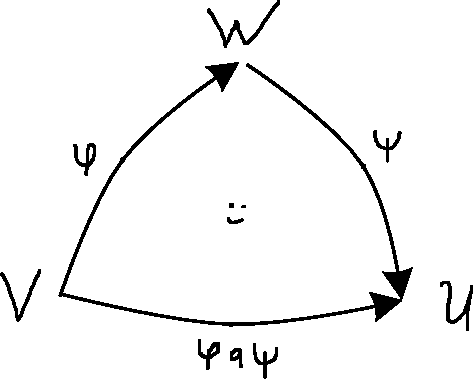
\includegraphics[width=5.5cm]{image/lecture-10.pdf}$$
    Зададим отображение по правилу: 
    $$(\psi \circ \phi)(x) = \psi(\phi(x)) \tab[0.3cm] \forall x \in V$$   
    \begin{subtheorem}
      Отображение $\psi \circ \phi: V \to U$ является линейным.
    \end{subtheorem} 
    \begin{proof}
      $\forall a, b \in V$
      \begin{enumerate}
        \item $(\psi \circ \phi)(a+b) = \psi(\phi(a+b)) = \psi(\phi(a)+\phi(b)) = \psi(\phi(a))+\psi(\phi(b))$ 
        \item Аналогично для $(\psi \circ \phi)(\lambda a) = \lambda(\psi \circ \phi)(a)$ 
      \end{enumerate}
    \end{proof} 

    Фиксируем базис: \tab[0.3cm]$\mathcal{E} = \{e_1,...,e_n\}$ - базис в $V$ \\
    \tab[4.3cm]$\mathcal{F} = \{f_1,...,f_m\}$ - базис в $W$ \\
    \tab[4.3cm]$\mathcal{G} = \{g_1,...,g_k\}$ - базис в $U$ \\
    $\underset{m \times n}{A}$ - матрица линейного отображения $\phi$ относительно $\mathcal{E}, \mathcal{F}$. \\
    $\underset{k \times m}{B}$ - матрица линейного отображения $\psi$ относительно $\mathcal{F}, \mathcal{G}$. \\
    $\underset{k \times n}{C}$ - матрица линейного отображения $\psi \circ \phi$ относительно $\mathcal{E}, \mathcal{G}$.
    \begin{subtheorem}
      $C = B \cdot A$ 
    \end{subtheorem} 
    \begin{proof}
      $$\phi(e_i) = \sum \limits_{s=1}^ma_{si}f_s; \tab[1cm]\psi(f_s) = \sum \limits_{t=1}^kb_{ts}g_t$$
      По определению матрицы линейного отображения:
      $$(\psi \circ \phi)(e_i) = \sum \limits_{l=1}^kc_{li}g_l \tab[0.3cm](\ast)$$ 
      По определению композиции:
      $$(\psi \circ \phi)(e_i) = \psi(\phi(e_i)) = \psi(\sum \limits_{s=1}^ma_{si}f_s) = \sum \limits_{s=1}^ma_{si}\psi(f_s) =\tab[4cm]$$ $$\tab[7cm]= \sum \limits_{s=1}^ma_{si}(\sum \limits_{t=1}^kb_{ts}g_t) = \sum \limits_{t=1}^k(\sum \limits_{s=1}^mb_{ts}a_{si})g_t \tab[0.3cm](\star)$$
      $\Longrightarrow $$(\ast) = (\star)$.\\
      Т.к. координаты определены однозначно $\Rightarrow c_{it} = \sum \limits_{s=1}^mb_{ts}a_{si} \Rightarrow C =B \cdot C$  
    \end{proof} 
  \end{itemize}
  \subsection{Свойства операций над матрицами}
  Предположим, что все размеры матриц согласованы. 
  \begin{enumerate}
    \item $M_{m \times n}(\R)$ - векторное пространство над $\R$
    \item Ассоциативность  $A(BC) = (AB)C$ 
    \begin{proof}
    $\underset{m \times k}{A} , \tab[0.1cm]\underset{k \times n}{B} , \tab[0.1cm]\underset{n \times l}{C}$ $\vspace{0.1cm}$

    Пусть $\underset{m \times l}{D} = A(BC), \tab[0.1cm]\underset{m \times l}{\widetilde{D}} = (AB)C$. 
    Надо проверить, что $\forall i,j: [D]_{ij} = [\widetilde{D}]_{ij}$. 
    $$[D]_{ij} = [A(BC)]_{ij} = \sum \limits_{s=1}^k[A]_{is} \cdot [BC]_{si} = \sum \limits_{s=1}^k[A]_{is}(\sum \limits_{t=1}^n[B]_{st} \cdot [C]_{ti}) = $$ $$  = \sum \limits_{s=1}^k \sum \limits_{t=1}^n[A]_{ij}([B]_{st} \cdot [C]_{ti})$$ 
    $$[\widetilde{D}]_{ij} = [(AB)C]_{ij} = \sum \limits_{t=1}^n[AB]_{it}[C]_{tj} = \sum \limits_{t=1}^n (\sum \limits_{s=1}^k[A]_{is} \cdot [B]_{st})[C]_{tj} = $$
    $$ = \sum \limits_{t=1}^n \sum \limits_{s=1}^k ([A]_{is} \cdot [B]_{st}) \cdot [C]_{tj}$$  
    По свойствам операций над $\R$ результаты преобразований равны.
    \end{proof} 
    \item $A(B+C) = AB + AC$
    \item $(B + C)A = BA + CA$  
    \item $\lambda(AB) = (\lambda A) B = A(\lambda B); \tab[0.3cm]\forall \lambda \in \R$ 
    \item $\forall A \in M_{m \times m}(\R)$, $\exists$  единичная матрица $E \in M_{m \times m}(\R)$ : 
    $EA = A$  
    \item $\forall A \in M_{m \times n}(\R)$ : $0 \cdot A = 0$ 
    \item Нет коммутативности: $AB \neq BA$ даже если размеры согласованы 
    \begin{proof}
      Свойства 3. - 7. упражнение)
    \end{proof} 
  \end{enumerate}
  \subsection{Свойства операции транспонирования}
  \begin{enumerate}
    \item $(A^T)^T = A$
    \item $(\lambda A)^T = \lambda A^T$
    \item $(A+B)^T = A^T + B^T$
    \item $(AB)^T = B^TA^T$   
    \begin{proof}
      4. $\underset{m \times k}{A}, \underset{k \times n}{B} \Longrightarrow \underset{n \times k}{B^T}, \underset{k \times m}{A^T}$ (размеры совпадают) \\
      Проверим равенство $D = (AB)^T \text{ и } \widetilde{D} = B^TA^T$.
      $$[D]_{ij} = [(AB)^T]_{ij} = [(AB)]_{ji} = \sum \limits_{s=1}^k[A]_{js}[B]_{si}$$ 
      $$[\widetilde{D}]_{ij} = B^TA^T = \sum \limits_{s=1}^k[B]_{is}[A]_{sj} = \sum \limits_{s=1}^k[A]_{js}[B]_{si}$$ 
    \end{proof} 
  \end{enumerate}
  \subsection{О ранге и операциях над матрицами}
  \begin{theorem} \tab
    \begin{enumerate}
      \item $rkA^T = rkA$
      \item $rk(\lambda A) = \begin{cases}
        rkA, \ \text{если } \lambda \neq 0 \\
        0, \ \text{если } \lambda = 0
      \end{cases}
      $ 
      \item $rk(A+B) \leq rkA + rkB$ 
      \item $rk(AB) \leq \min\{rkA, rkB\}$ 
    \end{enumerate}
  \end{theorem}  
    
  \begin{proof} \tab
    \begin{enumerate} 
      \item Следует из того, что ранг системы строк = рангу системы столбцов, и из определения ранга матрицы.
      \item Очев. 
      \item Пусть $\overline{a_1},...,\overline{a_m}$ - строки матрицы $A$. $\overline{b_1},..,\overline{b_m}$  - строки матрицы $B$. \\
      $\overline{a_1} + \overline{b_1} ,..., \overline{a_m} + \overline{b_m}$ - строки матрицы $A+B$. 
      $$rkA = \dim \langle \overline{a_1},...,\overline{a_m} \rangle, \ rkB = \dim \langle \overline{b_1},...,\overline{b_m} \rangle$$   
      $$rk(A+B) = \dim \langle \overline{a_1} + \overline{b_1} ,..., \overline{a_m} + \overline{b_m} \rangle$$ 
      Заметим, что $(\langle \overline{a_1} + \overline{b_1} ,..., \overline{a_m} + \overline{b_m} \rangle) \subseteq (\langle \overline{a_1},...,\overline{a_m}, \overline{b_1},...,\overline{b_m} \rangle)$   
      \begin{lemma}
        Пусть $V$ векторное пространсво над $\R$ $\dim V = n$  \\
        $U$ -  произвольное подпространство в $V$. Тогда $\dim U \leq n$ \\
        Более того, если $U \neq V$, то $\dim U<n$.
      \end{lemma} 
      \begin{proof} 
        Пусть $\{e_1,...,e_m\}$ - базис $U \subseteq V$, т.е. $\dim U = m$ \\
        ЛНЗ систему $\{e_1,...,e_m\}$ можно дополнить до базиса в $V$ $\Longrightarrow m\leq n$  \\
        Если $m = n$, то $\{e_1,...,e_m\}$ - базис $V \Longrightarrow V=U$
      \end{proof} 
      Применяем лемму и получаем, что 
      $$\dim\langle \overline{a_1} + \overline{b_1} ,..., \overline{a_m} + \overline{b_m} \rangle \leq \dim\langle \overline{a_1},...,\overline{a_m}, \overline{b_1},...,\overline{b_m} \rangle$$ 
      Т.к. объединение базисов линейной оболочки $\overline{a_1},...,\overline{a_m}$ и $\overline{b_1},..,\overline{b_m}$ является конечной порождающей системой линейной оболочки $\langle \overline{a_1},...,\overline{a_m}, \overline{b_1},...,\overline{b_m} \rangle$, а из любой конечной порождающей системы можно выбрать базис, значит: $$\dim\langle \overline{a_1} + \overline{b_1} ,..., \overline{a_m} + \overline{b_m} \rangle \leq \dim\langle \overline{a_1},...,\overline{a_m} \rangle + \dim\langle \overline{b_1},...,\overline{b_m} \rangle$$ $$\Longrightarrow  rk(A+B) \leq rkA + rkB$$
      \item Докажем, что $rkAB \leq rkA$. Пусть $C =AB$, $\underset{m \times k}{A}, \underset{k \times n}{B}$ \\
      $A_1,...,A_n$ - столбцы матрицы $A$ \\
      $B_1,...,B_n$ - столбцы матрицы $B$ \\
      $C_1,...,C_n$ - столбцы матрицы $C$
      $$C_1 = AB_1 = A_1b_{11} + \cdots + A_kb_{k1}$$ 
      $$C_2 = AB_2 = A_1b_{12} + \cdots + A_kb_{k2}$$
      $$\vdots$$
      $$C_n = AB_n = A_1b_{1n} + \cdots + A_kb_{kn}$$
      $\Longrightarrow \langle C_1,...,C_n \rangle \subseteq \langle A_1,...,A_k \rangle \Longrightarrow \dim\langle C_1,...,C_n \rangle \leq \dim\langle A_1,...,A_k \rangle \Longrightarrow rkC\leq rkA$. \\
      Докажем, что $rkAB \leq rkB$.
      $$rk(AB) = rk(AB)^T = rk(B^TA^T) \leq rkB^T = rkB$$ 
    \end{enumerate}
  \end{proof} 
  \section{Перестановки}
  \begin{definition}
    Упорядоченная последовательность $(k_1,...,k_n)$ чисел $1,2,...,n$, расположенных в некотором порядке, называется перестановкой из $n $ элементов. 
  \end{definition} 
  \begin{example1}
    $(3,1,2)$ перестановка из 3-х элементов. 
  \end{example1}
  \begin{definition}
    Перестановка $(1,2,...,n)$ называется тривиальной.
  \end{definition} 
  \begin{definition}
    Говорят, что пара элементов $k_i \text{ и } k_j$ образуют инверсию, если: 
    $$i<j \Longrightarrow  k_i>k_j$$
  \end{definition} 
  \begin{definition}
    Перестановка называется четной (нечетной), если число инверсий в ней четное (нечетное).\\
    Знак переставки - $\textrm{sgn}(k_1,...,k_n) = (-1)^s$, где $s$ - число инверсий в перестановке. 
  \end{definition} 
  \begin{definition}
    Перемена двух элементов в перестановке называется транспозицией этих элементов.
  \end{definition} 
  \begin{subtheorem}
    При транспозиции любых двух элементов четность меняется на противоположную.
  \end{subtheorem} 
  \begin{proof} $\tab$ 
    \begin{enumerate} 
      \item Транспозиция двух соседних элементов. \\
      При этом изменится расположение только этих элементов относительно других $\Longrightarrow $ количество инверсий изменился на 1 $\Longrightarrow $ четность поменяется. 
      \item Общий случай: 
      $$(...,k_i,...,k_j,...) \to (...,k_j,...,k_i,...)$$ 
      Пусть между $k_i \text{ и } k_j$ (s) элементов. \\
      Перемену $k_i \text{ и } k_j$ произведем за $2s+1$ транспозицию соседних элементов. \\
      Сначала $k_i$ переставим последовательно с каждым из элементов, стоящих между $k_i \text{ и } k_j$ (это $s$ транспозиций), потом $k_i$ переставим с $k_j$, затем $k_j$ поставим на $i$ позицию (это еще $s$ транспозиций). \\
      Т.к. транспозиция соседних элементов меняет четность, то за $2s+1$ транспозицию четность изменится.
    \end{enumerate}
  \end{proof} 
  \begin{consequense}
    Пусть $n>1$. Тогда число четных перестановок из $n$ элементов равно числу нечетных. 
  \end{consequense} 
  \begin{proof}
    Перечислим все четные перестановки и в каждой поменяем местами первые 2 элемента. При этом получим различные нечетные перестановки $\Longrightarrow $ число четных перестановок $\leq$ числа нечетных. Аналогично в обратную сторону. \\
    $\Longrightarrow $ число четных = число нечетных. 
  \end{proof} 
  \begin{subtheorem}
    Число перестановок из $n$ элементов равно $n!$ 
  \end{subtheorem} 
  \begin{proof}
    $(k_1,...,k_n)$ для $k_1$ вариантов - $n$  \\
    Пусть выбрали $k_1 \Longrightarrow$ для  $k_2$ вариантов - $n-1$ и т.д. Получаем всего вариантов: $n\cdot(n-1)\cdot ... \cdot 1 = n! $ 
  \end{proof} 

  \section{Определители n-го порядка}
  \begin{definition}
    Определителем квадратной матрицы $\underset{n \times n}{A}=(a_{ij})$ порядка $n$ называется число, которое вычисляется по формуле:
    $$|A|=\det{A}=\sum\limits_{(k_1,\dots,k_n)}\textrm{sgn}(k_1,\dots,k_n)a_{1k_1}a_{2k_2}\dots a_{1k_n}$$
    Где $\sum\limits_{(k_1,\dots,k_n)}$ - сумма по всем перестановкам из $n$ элементов. Эта формула называется формулой полного разложения или полного развертывания определителя.
  \end{definition}
  \begin{example1}
    $$\begin{vmatrix}
      a_{11} & a_{12}\\
      a_{21} & a_{22}  
    \end{vmatrix} = \textrm{sgn}(1,2)a_{11}a_{22}+\textrm{sgn}(2,1)a_{12}a_{21}=a_{11}a_{22}-a_{12}a_{21}$$
  \end{example1}
  $$\underset{n \times n}{A}=\begin{pmatrix}
    \tab & \overline{a_1} & \tab\\
    \null & \overline{a_2} & \null\\
    \null & \vdots & \null\\
    \null & \overline{a_n} & \null
  \end{pmatrix}$$
  Пусть $\overline{a_1}, \overline{a_2}, \dots \overline{a_n}$ - строки матрицы $A$. Тогда определитель можно рассматривать как функцию от строк $\det{A}=\det{(\overline{a_1},\overline{a_2},\dots \overline{a_n})}$
  \begin{definition}
    Функция $f(v_1,\dots, v_n)$, которая векторам $v_1,\dots, v_n$ в вектроном простанстве $V$ над $\R$ ставит в соответствие число из $\R$, то есть $f:V\times\dots\times V\to \R$
    называется полилинейной, если она линейна по каждому аргументу, т.е. для каждого $i=\overline{1,n}$ выполнено:
    \begin{enumerate}
      \item $f(v_1,\dots, v_i+\widetilde{v_i},\dots, v_n)=f(v_1,\dots, v_i,\dots, v_n)+f(v_1,\dots, \widetilde{v_i},\dots, v_n),\\ \forall v_i, \widetilde{v_i}\in V$.
      \item $f(v_1,\dots, \lambda v_i,\dots, v_n)=\lambda f(v_1,\dots, v_i,\dots, v_n),\ \forall \lambda\in \R,\ \forall v_i\in V$.
    \end{enumerate}
  \end{definition}
  \begin{definition}
      Полилинейная функция $f:V\times\dots\times V\to \R$ называется кососимметричной, если при перестановке любых двух аргументов значение функции умножается на $(-1)$. Кососимметричная функция с двумя одинаковыми аргументами равна нулю.
  \end{definition}
  \begin{example1}
    Если $f$ - кососимметричная функция и $v_1=v_2$, то\\
    $f(v_1,v_2,v_3,\dots, v_n)=-f(v_2,v_1,v_3,\dots, v_n)=a \Longrightarrow a=-a \Longrightarrow a=0$.
  \end{example1}

  \subsection{Свойства определителей}

  \setcounter{thcount}{0}

  \begin{theoremnum}
    Определитель $n$-го порядка является кососимметричной полилинейной функцией от строк матрицы.    
  \end{theoremnum} 
  \begin{proof}
    $$A=\begin{pmatrix}
      \tab & \overline{a_1} & \tab\\
      \null & \overline{a_2} & \null\\
      \null & \vdots & \null\\
      \null & \overline{a_n} & \null
    \end{pmatrix}=(a_{ij}),\ \overline{a_i}=(a_{i1},\dots, a_{in})$$
    $$\det{A}=\det{(\overline{a_1},\dots \overline{a_n})}=\sum\limits_{(k_1,\dots k_n)}\textrm{sgn}(k_1,\dots k_n)a_{1k_1}\dots a_{nk_n}$$
    Докажем, что $\det{A}$ линеен по $i$-му аргументу.
    $$\det{A}=\sum\limits_{k=1}^na_{ik}u_k$$
    где $u_k$ - число, не зависящее от элементов строки $\overline{a_i}$
    \begin{multline*}
      1.\ \det(\overline{a_1},\dots,\overline{a_i}+{\overline{a_i}}^{\prime},\dots, \overline{a_n})=\sum\limits_{k=1}^n(a_{ik}+a_{ik}^{\prime})u_k=\sum\limits_{k=1}^na_{ik}u_k+\sum\limits_{k=1}^na_{ik}^{\prime}u_k=\\=\det{(\overline{a_1},\dots,\overline{a_i},\dots, \overline{a_n})}+\det{(\overline{a_1},\dots,\overline{a_i}^{\prime},\dots, \overline{a_n})}
    \end{multline*}
    $$2.\ \det{(\overline{a_1},\dots,\lambda\overline{a_i},\dots, \overline{a_n})}=\sum\limits_{k=1}^n(\lambda a_{ik})u_k=\lambda\sum\limits_{k=1}^na_{ik}u_k=\lambda\det{(\overline{a_1},\dots,\overline{a_i},\dots, \overline{a_n})}$$
    Теперь докажем кососимметричность:
    \begin{multline*}
    \det{(\overline{a_1},\dots,\underset{(a_i)}{\overline{a_j}},\dots,\underset{(a_j)}{\overline{a_i}},\dots,\overline{a_n})}=\\ \tab[-2.8cm]=\sum\limits_{(k_1\dots k_i\dots k_j\dots k_n)}\textrm{sgn}(k_1,\dots k_n)a_{1k_1}\dots a_{jk_i}\dots a_{ik_j}\dots a_{nk_n}=\\=\sum\limits_{(k_1\dots k_i\dots k_j\dots k_n)}\textrm{sgn}(k_1,\dots k_n)a_{1k_1}\dots a_{ik_j}\dots a_{jk_i}\dots a_{nk_n}=\\=-\sum\limits_{(k_1\dots k_i\dots k_j\dots k_n)}\textrm{sgn}(k_1,\dots k_n)a_{1k_1}\dots a_{ik_i}\dots a_{jk_j}\dots a_{nk_n}=\tab[-2.8cm]\\=-\det{(\overline{a_1},\dots,\overline{a_i},\dots,\overline{a_j},\dots,\overline{a_n})}
    \end{multline*}
  \end{proof} 
  \begin{theoremnum}
    Пусть $f(A)=f(\overline{a_1},\dots,\overline{a_n})$ - функция от строк, $A\in M_n(\R)$ такие, что:
    \begin{enumerate}
      \item $f(E)=1$
      \item $f$ - Полилинейная
      \item $f$ - Кососимметричная
    \end{enumerate}
      тогда $f(A)=\det{A}$.
  \end{theoremnum}
  \begin{proof}
    $e_1 = (1,0,...,0),...,e_n=(0,...,0,1)$ - строки единичной матрицы $E = \begin{pmatrix}
      1 & \null & 0\\
      \null & \ddots & \null \\
      0 & \null & 1
    \end{pmatrix} \Longrightarrow  \{e_1,...,e_n\}$ - базис в векторном пространстве $\R^n$ 
    $$\Longrightarrow \overline{a_i} = (a_{i1},...,a_{in}) = a_{i1}e_1 + \cdots + a_{in}e_n$$
    $$\Longrightarrow f(A) = f(\overline{a_1},...,\overline{a_n}) = f(\sum \limits_{k_1=1}^na_{1k_1}e_{k_1}, ..., \sum \limits_{k_n=1}^na_{nk_n}e_{k_n}) = $$
    $$= \sum \limits_{k_1=1}^n ... \sum \limits_{k_n=1}^n a_{1k_1}\cdot ... \cdot a_{nk_n}\cdot f(e_{k_1},...,e_{k_n}) =$$
    $$= \sum \limits_{(k_1,...,k_n)}f(e_{k_1},...,e_{k_n})\cdot a_{1k_1}\cdot ... \cdot a_{nk_n}$$ 
    Осталось доказать, что $f(e_{k_1},...,e_{k_n}) = \textrm{sgn}(k_1,...,k_n)$. \\
    Т.к. $f(E) =1$, то $f(A) = f(e_1,e_2,...,e_n) = \textrm{sgn}(1,2,...,n) (*)$   \\
    Меняя любые два аргумента местами, $f$ меняет знак, т.к. $f$ кососимметрична. С другой стороны, меняя два любые числа перестановки местами, знак перестановки $\textrm{sgn}$ тоже меняет знак. \\
    Любую перестановку можно получить из тривиальной за конечное число транспозиций. \\
    Т.к. $(*)$ верно, то, делая последовательно транспозицию в перестановке, и такую же перемену аргументов у функции $f$, получим $f(e_{k_1},...,e_{k_n}) = \textrm{sgn}(k_1,...,k_n)$. 
  \end{proof} 
  \begin{consequense} \tab
    \begin{enumerate}
      \item Если в квадратной матрице $A$ одна из строк равна линейной комбинации остальных, то $detA = 0$
      \item Если к строке квадратной матрицы $A$ применить ЭП1 (т.е. к строке прибавить другую, умноженную на число), то определитель не изменится. 
    \end{enumerate}
  \end{consequense} 
  \begin{proof} \tab
    \begin{multline*}
      2) \ det(\overline{a_1},...,\overline{a_i}+\lambda \overline{a_j},...,\overline{a_n}) = \\ = det(\overline{a_1},...,\overline{a_i},...,\overline{a_j},...,\overline{a_n}) + \lambda det(\overline{a_1},...,\overline{a_j},...,\overline{a_j},...,\overline{a_n}) = \\ = det(\overline{a_1},...,\overline{a_i},...,\overline{a_j},...,\overline{a_n})
    \end{multline*}
  \end{proof} 
  \begin{definition}
    Квадратная матрица $A = (a_{ij})$ называется верхнетреугольной (нижнетреугольной) матрицей, если $a_{ij} = 0$ при $i>j$. 
    \begin{example1}
      $\begin{pmatrix}
        1 & 2 & 3 \\ 0 & 4 & 2 \\ 0 & 0& 0
      \end{pmatrix}$
    \end{example1}  
  \end{definition} 
  Можно проследить, как влияют ЭП на определитель:
  \begin{itemize}
    \item ЭП1 = $\overline{a_i} \to \overline{a_i} + \lambda \overline{a_j}$ \tab[0.3cm] $det$ не изменится. 
    \item ЭП2 $\overline{a_i} \to \overline{a_j}$ \tab[2.15cm] $det$ умножается на -1. 
    \item ЭП3 $\overline{a_i} \to \mu \overline{a_i}, \mu \not = 0$ \tab[0.45cm] $det$ умножится на $\mu$. 
  \end{itemize}
  \begin{subtheorem}
    Определитель верхней треугольной матрицы равен произведению диагональных элементов.
  \end{subtheorem} 
  \begin{proof}
    $\begin{vmatrix}
      a_{11} & a_{12} & \cdots & a_{1n} \\
      0 & a_{22} & \cdots & a_{2n} \\
      \null & \null & \ddots & \null \\
      0 & 0 & \cdots & a_{nn} 
    \end{vmatrix} = a_{11}\cdot a_{22}\cdot...\cdot a_{nn}$ \\
    Рассмотрим любую не тождественную перестановку $(k_1,...,k_n)$, где $k_i \not = i$. Тогда найдется такой множитель $(i>j) \ a_{ij} = 0,  \Longrightarrow $ это слагаемое обнулится. $\Longrightarrow $ Во всей сумме останется только тождественная перестановка. 
  \end{proof} 

  \begin{theoremnum}
    Определитель при транспонировании не изменяется: $detA = detA^T$
  \end{theoremnum} 

  \begin{proof}
    Пусть $B = A^T, \ a=(a_{ij}), \ B=(b_{ij})$ \\
    $detA = \sum \limits_{(l_1,...,l_n)}\textrm{sgn}(l_1,...,l_n)a_{1l_1},...,a_{nl_n}$
    \begin{multline*}
      detA^T = detB = \sum \limits_{(k_1,...,k_n)}\textrm{sgn}(k_1,...,k_n)b_{1k_1},...,b_{nk_n} = \\
      = \sum \limits_{(k_1,...,k_n)}\textrm{sgn}(k_1,...,k_n)a_{k_11},...,a_{k_nn} = \tab[0.8cm]\\ 
      = \sum \limits_{(k_1,...,k_n)}\textrm{sgn}(k_1,...,k_n) \textrm{sgn}(1,2,...,n)a_{k_11},...,a_{k_nn} = (*)
    \end{multline*} 
    Переставим $a_{ij}$, переупорядочив номера строк, т.е. первые индексы по возрастанию последовательно, меняя два множителя местами: $$a_{k_11},...,\underbrace{a_{k_ii},...,a_{k_jj}}_{\text{меняем}},...,a_{k_nn}$$ 
    При этой перемене двух множителей местами меняются местами и первые индексы, и вторые. При этом: 
    \begin{multline*}
      \textrm{sgn}(k_1,...,k_i,...,k_j,...,k_n) \cdot \textrm{sgn}(1,...,i,...,j,...,n) = \\ = (-1)^2 \textrm{sgn}(k_1,...,k_j,...,k_i,...,k_n)\cdot \textrm{sgn}(1,...,j,...,i,...,n)
    \end{multline*}
    $(*) = \sum \limits_{(l_1,...,l_n)} \textrm{sgn}(1,2,...,n) \textrm{sgn}(l_1,...,l_n) a_{1l_1},...,a_{nl_n} = detA$
  \end{proof} 
  \begin{consequense}
    Определитель матрицы есть кососимметричная и полилинейная функция столбцов матрицы. \\
    Все свойства определителя, которые верны для строк матрицы, верны и для столбцов.
  \end{consequense} 

  \subsection{Элементарные матрицы}
  \begin{definition}
    Матрица, полученная из единичной матрицы $E$, с помощью одного элементарного преобразования над строками или столбцами, называется элементарной матрицей. \\
    ЭП1: \ $\overline{a_i} \to \overline{a_i} + \lambda \overline{a_j}, \ \ i \not = j$
    $$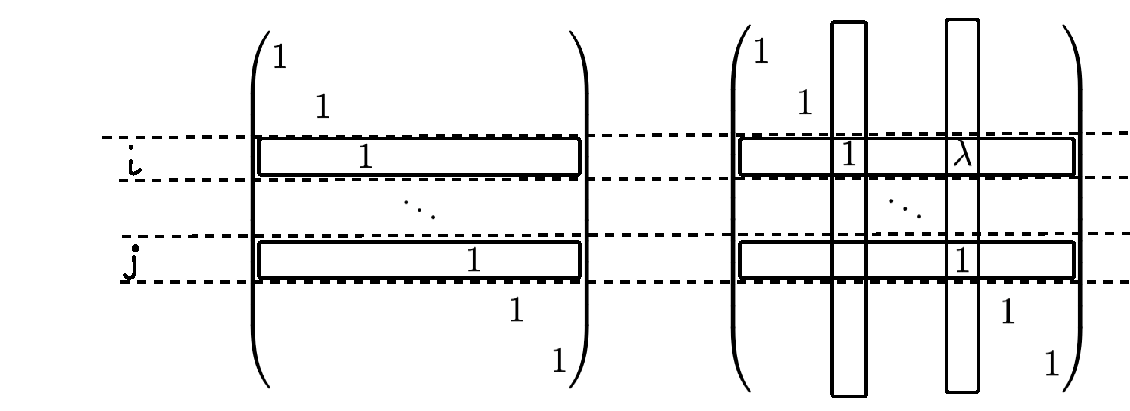
\includegraphics[width=12cm]{image/lecture-11.pdf}$$
    ЭП2: $\overline{a_i} \leftrightarrow  \overline{a_j}, \ \ i \not = j$ \tab[2.5cm] ЭП3: $\overline{a_i} \leftrightarrow \mu \overline{a_i}, \ \ \mu \not = 0$ \\
    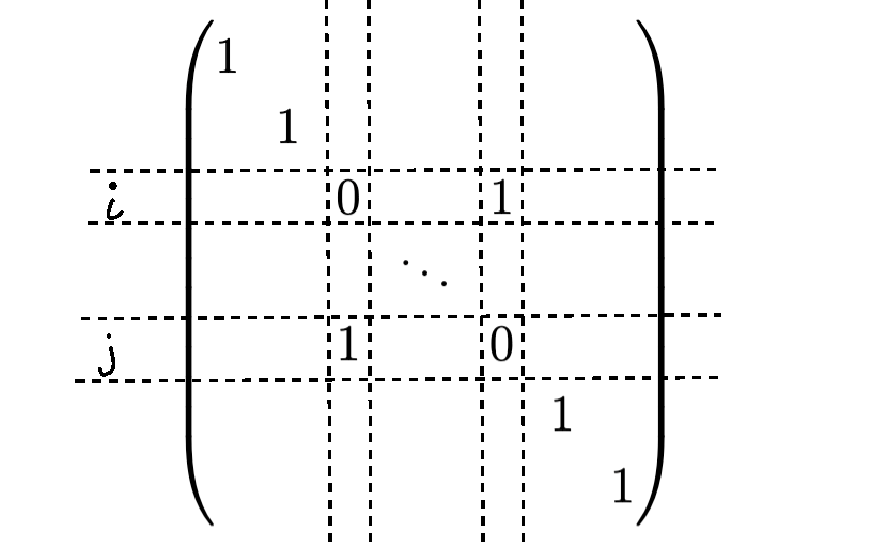
\includegraphics[width=7cm]{image/lecture-12.pdf}
    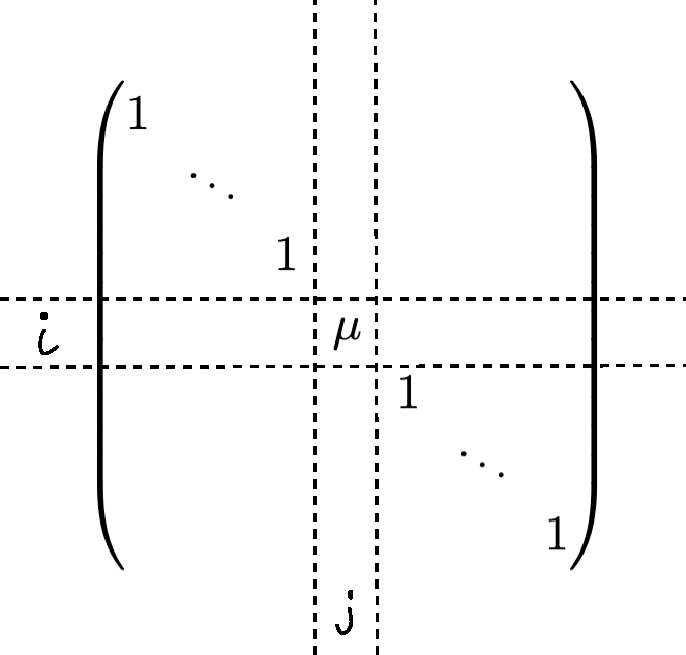
\includegraphics[width=5.6cm]{image/lecture-13.pdf}
  \end{definition} 
  % \setcounter{lemcount}{0}
  \begin{lemmanum2}  \label{lemma1} \tab 
    \begin{itemize}
      \item[\textbf{1.1}] Любые ЭП над строками матрицы $A$ равносильны умножению матрицы $A$ слева на элементарную матрицу, т.е. \\
      $A \leadsto  \widetilde{A} \Longleftrightarrow \widetilde{A} = T \cdot A$ где $T$ - элементарная матрица, такая что $E \leadsto  T$
      \item[\textbf{1.2}] Любые ЭП над столбцами матрицы $A$ равносильны умножению матрицы $A$ справа на элементарную матрицу.
    \end{itemize}
  \end{lemmanum2} 
  \begin{proof}
    Непосредственная проверка
  \end{proof}
  \begin{lemmanum2} \label{lemma2}
    Пусть $A$ - квадратная матрица порядка $n$, тогда:
    \begin{enumerate}
      \item Если $detA \not = 0$, то с помощью ЭП над строками $A$ можно привести к $E$. 
      \item Если $detA = 0$, то с помощью ЭП над строками в $A$ можно получить нулевую строку
    \end{enumerate}
  \end{lemmanum2} 
  \begin{proof}
    Методом Гаусса любую матрицу можно привести к ступенчатому виду. Ступенчатый вид для квадратной матрицы является верхнетреугольной, т.е.:
    $$A \leadsto \widetilde{A} = \begin{pmatrix}
      \widetilde{a_{11}} & \null & * \\
      \null & \ddots & \null \\
      0 & \null & \widetilde{a_{nn}}
    \end{pmatrix}$$  
    $\Longrightarrow detA = \xi \cdot det \widetilde{A}$, где $\xi \not = 0$, \ $det \widetilde{A} = \widetilde{a_{11}} \cdot ... \cdot \widetilde{a_{nn}}$\\
    Итак, 
    $$detA =0 \Longleftrightarrow  det \widetilde{A} = 0 \Longleftrightarrow \widetilde{a_{11}} \cdot ... \cdot \widetilde{a_{nn}} =0$$ 
    \begin{enumerate}
      \item Если $detA \not = 0$, то $a_{11} \not = 0,...,a_{nn} \not = 0$ - лидеры матрицы $A$ \\ $\Longrightarrow \widetilde{A}$  приводится к улучшенному ступенчатому виду обратным ходом Гаусса и этот улучшенный ступенчатый вид совпадает с $E$
      \item Если $detA = 0$, то $a_{11} \cdot...\cdot a_{nn} = 0$ $\Longrightarrow  \exists k: a_{kk} = 0$. По определению ступенчатого вида $\forall i > k: \widetilde{a_{ii}} = 0 \Longrightarrow \widetilde{a_{nn}} = 0 \Longrightarrow$ последняя строка в $\widetilde{A}$ нулевая.  
    \end{enumerate}
  \end{proof} 
  \begin{theoremnum}
    Пусть $A, B$ - квадратные матрицы порядка $n$, тогда: $$detAB = detA \cdot detB$$ 
  \end{theoremnum} 
  \begin{proof}
    Из ассоциативности умножения $T(AB) = (TA)B$, где $T$ элементарная матрица, получаем, что элементраное преобразование над строками матрицы $A$ соответствует элементарному преобразованию строк матрицы $AB$.  
    \begin{itemize}
      \item[1 случай.] $detA = 0$ (по лемме \eqref{lemma1}, пункт 2)$\Longrightarrow A\leadsto \widetilde{A}$( с нулевой строкой) \\
      $\Longrightarrow \widetilde{A} = \cdot(T_1 \cdot ... \cdot T_k)\cdot A, \ $ где $T_i$ - матрицы элементарных преобразований. \\
      $\Longrightarrow (T_1 \cdot ... \cdot T_k)(AB) = ((T_1 \cdot ... \cdot T_k)A)B = \widetilde{A}B$ $\Longrightarrow det AB =0$, т.к. $AB \leadsto \widetilde{A}B$ 
      \item[2 случай.] $detA \not =$ 0 (по лемме \eqref{lemma1}, пункт 1) $\Longrightarrow A\leadsto E \Longrightarrow E=(T_1 \cdot ... \cdot T_k)A$, \ где $T_i$ - матрицы элементарных преобразований. \\
      $(T_1 \cdot ... \cdot T_k)(AB) = ((T_1 \cdot ... \cdot T_k)A)B = EB = B$ \\
      $\Longrightarrow detAB = c \cdot det((T_1 \cdot ... \cdot T_k)AB) = c \cdot detB$  \\
      Рассмотрим отношение: $$\frac{detAB}{detA} = (*) $$ 
      $\\$ Произведем над матрицей $A$ ЭП, которые приведут матрицу $A \leadsto E$, одновременно производим такие же ЭП над $AB$. 
       $$ (*) = \frac{detEB}{detE} = detB$$ 
    \end{itemize}
  \end{proof} 
  \begin{theoremnum}
    (Об определителе с углом нулей) \\ Пусть $A$ - квадратная матрица порядка $k$ \\
    \tab[1.45cm]$B$ - квадратная матрица порядка $m$ \\
    \tab[1.45cm]$C$ - матрица размера $k \times m$. \\
    Тогда:
    $$det \begin{pmatrix}
      A & \vline & C \\
      \hline
      0 & \vline & B
    \end{pmatrix}(*) = detA \cdot detB$$ 
  \end{theoremnum} 

  \begin{proof} \tab
    \begin{itemize}
      \item[1 случай.] $detB = 0$ \\
      (По лемме \eqref{lemma2}, пункт 2) $B\leadsto \widetilde{B}$ 
      Производя точно такие же ЭП над последними $m$ строками матрицы $(*)$ , получаем нулевую строку $$\Longrightarrow det \begin{pmatrix}
        A & \vline & C \\
        \hline
        0 & \vline & B
      \end{pmatrix} = detA \cdot detB = 0$$  
      \item[2 случай.] $detA = 0$ Аналогично как в 1 случае, только ЭП над столбцами. 
      \item[3 случай.] $detA \not = 0, detB \not = 0$ \\
      Рассмотрим отношение:
      $$\frac{det \begin{pmatrix}
        A & \vline & C \\
        \hline
        0 & \vline & B
      \end{pmatrix}}{detA \cdot detB}$$\\ (По лемме \eqref{lemma2}, пункт 1) $A\leadsto E$, $B\leadsto E$ \\
      Преобразуем матрицу $A$ с помощью ЭП над столбцами, которые приводят $A \leadsto E$, преобразуем $B$ с помощью ЭП над строками, которые приводят $B \leadsto E$. Одновременно преобразуем матрицу $(*)$ с помощью таких же ЭП над строками и столбцами, отношение при этом не изменится. \\
      Тогда: 
      $$\frac{det \begin{pmatrix}
        A & \vline & C \\
        \hline
        0 & \vline & B
      \end{pmatrix}}{detA \cdot detB} =
      \frac{det \begin{pmatrix}
        E & \vline & C \\
        \hline
        0 & \vline & E
      \end{pmatrix}}{detE \cdot detE} = 1$$    
    \end{itemize}
  \end{proof} 

  \subsection{Разложение определителя по строке}

  $A$ - матрица размера $m \times n$. \\ 
  $i_1,...,i_k$ - номера некоторого разложения строк в $A$. \\ $j_1,...,j_t$ - номера некоторого разложения столбцов в $A$.
  \begin{definition}
    Матрица, состоящая из элементов матрицы $A$, стоящих на пересечении строк с номерами $i_1,...,i_k$ и столбцов с номерами $j_1,...,j_t$, называется подматрицей матрицы $A$\\
    Обозначение: 
    $A \begin{matrix}
      i_1 & \cdots & i_s \\
      \vdots & \null & \vdots \\
      j_1 & \cdots & j_t
    \end{matrix}$ 
  \end{definition}  
  \begin{definition}
    Минором $k-$ого порядка матрицы $A$ называется определитель квадратной подматрицы порядка $k$. 
  \end{definition} 
  
  \begin{example1}
    $$\begin{matrix}
      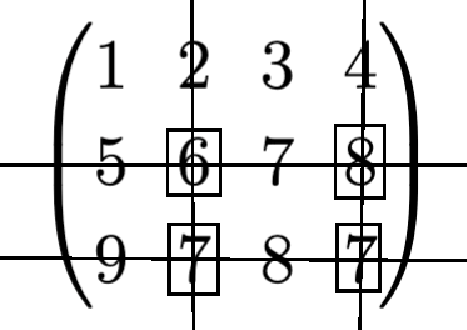
\includegraphics[width=3cm]{image/lecture-14.pdf} 
    \end{matrix}
    \Longrightarrow \text{Минор}= \begin{vmatrix}
      6 & 8 \\ 7 & 7
    \end{vmatrix}$$
  \end{example1}
  $\\$ 
  Пусть $A$ - квадратная матрица порядка $n$
  \begin{definition}
    Минор порядка $(n-1)$ квадратной матрицы $A$, порядка $n$, полученный вычеркиванием $i-$ой строки и $j-$ого столбца, называется дополнительным минором к элементу $a_{ij}$.  \\
    Обозначается: $M_{ij}$ 
  \end{definition}
  \begin{example1} 
    $$\begin{matrix}
      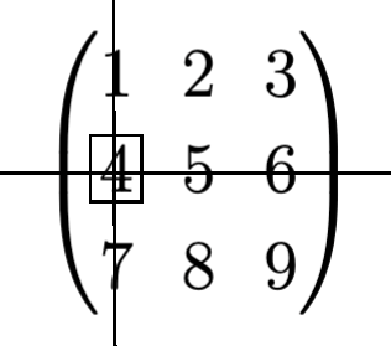
\includegraphics[width=3cm]{image/lecture-15.pdf}
    \end{matrix}
    \Longrightarrow M_{12} = \begin{vmatrix}
      2 && 3 \\ 8 && 9
    \end{vmatrix} = -6$$ 
  \end{example1}
  
  \begin{definition}
    Алгебраческое дополнение к элементу $a_{ij}$ - это число: $$A_{ij} = (-1)^{i+j} \cdot M_{ij}$$ 
  \end{definition} 
  \begin{example1}
    (к прошлому примеру) $A_{21} = (-1)^{2+1}(-6) = 6$  
  \end{example1}

  \begin{lemma}
    Матрица $\overline{A}$ , полученная из $A$ заменой $i-$ой строки на \\$(0,...,0,a_{ij},0,...,0)$:
    $$det \overline{A} = det \begin{pmatrix}
      \null & \null & \vdots & \null & \null \\
      0 & \cdots & a_{ij} & \cdots & 0 \\
      \null & \null & \vdots & \null & \null \end{pmatrix} = a_{ij} \cdot A_{ij}$$  
  \end{lemma} 
  \begin{proof}
    $$\begin{vmatrix}
      a_{11} & ... & ... & ... & a_{1n} \\
      \vdots & \null & \null & \null & \vdots & \\
      0 & ... & a_{ij} & ... & 0 \\
      \vdots & \null & \null & \null & \vdots & \\
      a_{n1} &  ... & ... & ... & a_{nn}
    \end{vmatrix} = (-1)^{i-1} \cdot (-1)^{j-1} \cdot \begin{vmatrix}
      a_{ij} \vline &  0 \\
      \hline 
      * \ \ \vline & B
    \end{vmatrix} = $$ $$ =(-1)^{i+j} \cdot a_{ij}\cdot detB = (-1)^{i+j} \cdot a_{ij} \cdot M_{ij} = a_{ij}\cdot A_{ij}$$
    где $B$ - подматрица $A$, из которой вычеркнули $i-$ую строку и $j-$ый столбец.
  \end{proof} 
  \begin{theoremnum}
    \begin{enumerate} \tab
      \item $detA = \sum \limits_{j=1}^na_{ij}A_{ij}$ - формула разложения по $i$-ой строке.
      \item $detA = \sum \limits_{i=1}^na_{ij}A_{ij}$ - формула разложения по $j$-ому столбцу.
    \end{enumerate}
  \end{theoremnum} 
  \begin{proof}
    $$detA = \begin{vmatrix}
      a_{11} & ... & ... & ... & a_{1n} \\
      \vdots & \null & \null & \null & \vdots & \\
      a_{i1} & ... & ... & ... & a_{in} \\
      \vdots & \null & \null & \null & \vdots & \\
      a_{n1} &  ... & ... & ... & a_{nn}
    \end{vmatrix} \overset{\text{В силу линейности}}{=} $$ 
    $$ = \begin{vmatrix}
      a_{11} & ... & ... & ... & a_{1n} \\
      \vdots & \null & \null & \null & \vdots & \\
      a_{i1} & 0 & ... & ... & 0 \\
      \vdots & \null & \null & \null & \vdots & \\
      a_{n1} &  ... & ... & ... & a_{nn}
    \end{vmatrix} + ... + \begin{vmatrix}
      a_{11} & ... & ... & ... & a_{1n} \\
      \vdots & \null & \null & \null & \vdots & \\
      0 & ... & ... & 0 & a_{in} \\
      \vdots & \null & \null & \null & \vdots & \\
      a_{n1} &  ... & ... & ... & a_{nn}
    \end{vmatrix} = $$ 
    $$ = a_{i1}A_{i1} + ... + a_{in}A_{in} = \sum \limits_{j=1}^na_{ij}A_{ij}$$ 
  \end{proof} 
  \subsection{Определитель Вандермонда}
  \begin{definition}
    $V(x_1,...,x_n$) - определитель Вандермонда.
    $$V(x_1,...,x_n) = \begin{vmatrix}
      1 & 1 & 1 & ... & 1 \\
      x_1 & x_2 & x_3 & ... & x_n \\
      x_1^2 & x_2^2 & x_3^2 & ... & x_n^2 \\
      \vdots & \vdots & \vdots & ... & \vdots \\
      x_1^{n-1} & x_2^{n-1} & x_3^{n-1} & ... & x_n^{n-1}
    \end{vmatrix} = \prod\limits_{1\leq i \leq j \leq n} (x_i - x_j)$$  
  \end{definition}
  

  Вычисление индукции по $n$ \\ 
  База: $n=2: \begin{vmatrix}
    1 & 1\\ x_1 & x_2 \end{vmatrix} = x_2 - x_1$ \\
  Пусть верно для $(n-1)$, тогда вычислим для $n$: 
  \begin{multline*}
    V(x_1,...,x_n) \overset{(1)}{=} \\ 
    \overset{(1)}{=} \begin{vmatrix}
      1 & 1 & 1 & ... & 1 \\
      0 & x_2-x_1 & x_3-x_1 & ... & x_n - x_1 \\
      0 & x_2^2 -x_1x_2 & x_3^2-x_1x_3 & ... & x_n^2-x_1x_n \\
      \vdots & \vdots & \vdots & ... & \vdots \\
      0 & x_2^{n-1}-x_1x_2^{n-2} & x_3^{n-1}-x_1x_3^{n-2} & ... & x_n^{n-1}-x_1x_n^{n-2}
    \end{vmatrix} \overset{(2)}{=} \tab[3cm]\\ 
    \overset{(2)}{=} \begin{vmatrix}
      x_2-x_1 & x_3-x_1 & ... & x_n - x_1 \\
      x_2^2 -x_1x_2 & x_3^2-x_1x_3 & ... & x_n^2-x_1x_n \\
      \vdots & \vdots & ... & \vdots \\
      x_2^{n-1}-x_1x_2^{n-2} & x_3^{n-1}-x_1x_3^{n-2} & ... & x_n^{n-1}-x_1x_n^{n-2}
    \end{vmatrix} \overset{(3)}{=} \tab[-0.2cm]\\
    \overset{(3)}{=} \begin{vmatrix}
    x_2-x_1 & x_3-x_1 & ... & x_n - x_1 \\
    x_2(x_2-x_1) & x_3(x_3-x_1) & ... & x_n(x_n-x_1) \\
    \vdots & \vdots & ... & \vdots \\
    x_2^{n-2}(x_2-x_1) & x_3^{n-2}(x_3-x_1) & ... & x_n^{n-2}(x_n-x_1)
    \end{vmatrix} =
  \end{multline*}
  \begin{multline*}
    = \prod\limits_{i=2}^{n}(x_i - x_1) \begin{vmatrix}
      1 & 1 & ... & 1\\
      x_2 & x_3 & ... & x_n\\
      \vdots & \vdots & ... & \vdots \\
      x_2^{n-2} & x_3^{n-2} & ... & x_n^{n-2}
      \end{vmatrix} = \\
      = \prod\limits_{i=2}^{n}(x_i - x_1)\prod\limits_{2\leq i \leq j \leq n} (x_i - x_j) = \prod\limits_{1\leq i \leq j \leq n} (x_i - x_j)
  \end{multline*}
  (1) Из каждой строки, начиная с последней, вычитаем предыдущую умноженную на $x_1$ \\
  (2) По теореме об определителе с уголом нулей \\
  (3) Выносим $(x_j - x_1)$ 
  \begin{consequense}
    (О фальшивом разложении определителя) \\
    Пусть $A = (a_{ij})$ - квадратная матрица порядка $n$, тогда:
    $$\sum \limits_{j=1}^n a_{ij}A_{kj} = 0 \text{ (при }i \not = k) (*)$$ 
    $$\sum \limits_{i=1}^n a_{ij}A_{ik} = 0 \text{ (при }j \not = k)$$ 
    $(*)$ - Т.е. алгебраическое дополнение берем из другой строки
  \end{consequense} 
  \begin{proof}
    Для сторок (для столбцов аналогично) 
    $$A = \begin{pmatrix}
      \null && \overline{a_1} && \null \\
      \null && \overline{a_2} && \null \\
      \null && \vdots && \null \\
      \null && \overline{a_n} && \null 
    \end{pmatrix}$$ 
    Рассмотрим матрицу $B$, где вместо $k$-ой строки стоит $i$-ая. 
    $$detB = \begin{vmatrix}
      \null && \overline{a_1} && \null \\
      \null && \vdots && \null \\
      \null && \overline{a_i} && \null \\
      \null && \vdots && \null \\
      \null && \overline{a_i} && \null \\
      \null && \vdots && \null \\
      \null && \overline{a_n} && \null  
    \end{vmatrix}
    =0 \text{ (т.к совпадающие строки)}$$ 
    С другой стороны, разложим $detB$ по $k$-ой строке: 
    $$B = (b_{ij}), \ detB = \sum \limits_{j=1}^nb_{kj}B_{kj} = \sum \limits_{j=1}^na_{ij}A_{kj}$$ 
  \end{proof} 
  \subsection{О ранге}
  \begin{definition}
    Квадратная матрица $A$ порядка $n$ называется невырожденной, если $rkA = n$ (т.е. её строки ЛНЗ, как и все столбцы)
  \end{definition}
  \begin{theoremnum}
    Квадратная матрица $A$ является невырожденной $\Longleftrightarrow detA \not = 0$ 
  \end{theoremnum}  
  \begin{proof}
    Пусть $A = (a_{ij})$ - квадратная матрица порядка $n$ \\
    Надо доказать, что $rkA=n \Longleftrightarrow detA \not = 0$ 
    \begin{itemize}
      \item[$\underline{\Longleftarrow} $] $detA \not = 0 \Longrightarrow $ (по лемме \eqref{lemma2}, пункт 1) $A \sim E \Longrightarrow rkA = rkE = n$
      \item[$\underline{\Longrightarrow} $] $rk = n$. Допустим, что $detA = 0 \Longrightarrow $ (по лемме \eqref{lemma2}, пункт 2) $A \sim \widetilde{A}$, где $\widetilde{A}$ - матрица с нулевой строкой $\Longrightarrow rkA = rk \widetilde{A} < n$. Противоречие $\Longrightarrow detA \not = 0$        
    \end{itemize}
  \end{proof} 
  \begin{consequense} \tab
    \begin{itemize}
      \item Все строки квадратной матрицы $A$ ЛНЗ $\Longleftrightarrow detA \not = 0$
      \item Все столбцы квадратной матрицы $A$ ЛНЗ $\Longleftrightarrow detA \not = 0$
    \end{itemize}
  \end{consequense} 
  \begin{theorem}
    (О ранге матрицы) \\
    Ранг матрицы $A$ совпадает с максимальным порядком отличного от нуля минора.
  \end{theorem}  
  \begin{proof}
    Пусть $rkA = r$ 
    \begin{itemize}
      \item Докажем, что все миноры порядка $s$, где $s>r$ равны нулю. \\
      Рассмотрим произвольный минор $M$ порядка $s$: $$M = det\begin{matrix}
        i_1 & \cdots & i_s \\
        \vdots & \null & \vdots \\
        j_1 & \cdots & j_s
      \end{matrix}$$ 
      т.к. $s>r$, то строки матрицы $A$ с номерами $i_1,...,i_s$ ЛЗ $\Longrightarrow $ строки, образующие минор, ЛЗ $\Longrightarrow M=0$ 
      \item Докажем, что $\exists$ хотя бы один ненулевой минор $\widetilde{M}$ порядка $r$. \\
      Т.к. $rkA = r$, то $\exists \ r$ ЛНЗ строк $\Longrightarrow rkB = r \Longrightarrow $ в $B \ \exists \ r $ ЛНЗ столбцов. Сформируем матрицу $C$ из этих столбцов $\Longrightarrow detC \not = 0$ \\
      $detC$ - это и есть искомый минор $\widetilde{M}$     
    \end{itemize}
  \end{proof} 
  \begin{definition}
     Пусть $M = detA \ \begin{matrix}
      i_1 & \cdots & i_s \\
      \vdots & \null & \vdots \\
      j_1 & \cdots & j_s
    \end{matrix}$ - минор порядка $s$ \\
    $i \not \in \{i_1,..,i_s\}, \ j \not \in \{j_1,..,j_s\}$ \vspace{0.3cm}\\
    $\widetilde{M} = detA \ \begin{matrix}
      i_1 & \cdots & i_s & i \\
      \vdots & \null & \null & \vdots \\
      j_1 & \cdots & j_s & j
    \end{matrix}$ - минор порядка  $s+1$ \\
    $\widetilde{M}$ - окаймляющий минор.  
  \end{definition} 
  \begin{example1}
    $$A = \begin{pmatrix}
      1 & 2 & 3 & 4 \\
      5 & 6 & 7 & 8 \\
      9 & 1 & 3 & 5 \\
      1 & -1 & 0 & 7
    \end{pmatrix}$$ 
    $M = detA \ \begin{matrix}
      1 & 3 \\ 2 & 4
    \end{matrix} = \begin{vmatrix}
      2 & 4 \\ 1 & 5
    \end{vmatrix} = 6$ \vspace{0.3cm}\\
    $\widetilde{M} = detA \ \begin{matrix}
      1 & 2 & 3 \\ 2 & 3 & 4
    \end{matrix} = \begin{vmatrix}
      2 & 3 & 4 \\ 6 & 7 & 8 \\ 1 & 3 & 5
    \end{vmatrix} = 0$  
  \end{example1}
  
  Метод окаймляющих миноров: \vspace{0.2cm}\\
  \tab[7cm]$\exists \ M_1 \not = 0 ?$ \vspace{0.15cm}\\
  \tab[5.5cm] да $\swarrow \tab[2.8cm] \searrow $ нет \vspace{0.15cm}\\
  \tab[4.6cm]$\exists \ M_2 \not = 0 ?$ \tab[2.6cm] $rkA =0$ \vspace{0.15cm}\\ 
  \tab[3.3cm] да $\swarrow \tab[2cm] \searrow $ нет \vspace{0.15cm} \\
  \tab[2.3cm]$\exists \ M_3 \not = 0 ?$ \tab[2cm] $rkA = 1$ \vspace{0.15cm}\\
  \tab[1cm] да $\swarrow \tab[2.8cm] \searrow $ нет \vspace{0.15cm}\\
  \tab[1.3cm]$...$ \tab[4cm] $...$
  \begin{subtheorem}
    Пусть $A = (a_{ij})$ - матрица размера $m \times n$, $\ \exists \ $ минор $M$ порядка $r$, отличный от нуля, и все миноры, окаймляющие его, равны нулю. \\
    Тогда $rkA = r$   
  \end{subtheorem} 
  \begin{proof}
    Пусть $M = detA \ \begin{matrix}
      i_1 & \cdots & i_r \\
      \vdots & \null & \vdots \\
      j_1 & \cdots & j_r
    \end{matrix}$. \vspace{0.3cm} Т.к. $M \not = 0$, то строки матрицы $A$ с номерами $i_1,...,i_r$ ЛНЗ $\Longrightarrow rkA \geq r$ \\
    Предположим, что $rkA \geq r+1$. Т.е. $\ \exists \ $ ЛНЗ строка (или больше). Рассмотрим строки $\overline{a_{i_1}},...,\overline{a_{i_r}}$, которые формируют минор $M$. Они ЛНЗ. \\
    Т.к. $rkA \geq r+1$, то $\ \exists \ i \not \in \{i_1,...,i_r\}: $ не выражаются линейно через \\ $\overline{a_{i_1}},...,\overline{a_{i_r}} \Longrightarrow \overline{a_{i_1}},...,\overline{a_{i_r}}$ - ЛНЗ. \\
    Образуем из этих строк матрицу $B \Longrightarrow rkB = r+1 \Longrightarrow \ \exists \ r+1$ ЛНЗ столбец. \\
    Столбцы с номерами $j_1,...,j_r$ ЛНЗ, т.к. $M \not = 0$ \\
    Т.к. $rkB = r+1$, то $\ \exists \ j \not \in \{j_1,...,j_r\}$: столбец с номером $j$ не выражается через столбцы с номерами $j_1,...,j_r$ \\
    Расмотрим подматрицу $C$ матрицы $B$, составленную из столбцов с номерами $j_1,...,j_r,j \Longrightarrow C-$ квадратная матрица порядка $r+1$ из ЛНЗ столбцов $\Longrightarrow detC \not = 0$\\
    $\Longrightarrow $ т.к. $det C $ является окаймляющим минора $M$, то получаем противоречие условию $\Longrightarrow rkA = r$.    
  \end{proof} 
  \subsection{Правила Крамера СЛУ}
  $\begin{cases}
    a_{11}x_1 + \cdots + a_{1n}x_n = b_1 \\
    \vdots \\ 
    a_{m1}x_1 + \cdots + a_{mn}x_n = b_n 
  \end{cases}$
  Матричная форма $AX=B$ \\ 
  СЛУ называется квадратной, если $m=n$ \\
  Пусть СЛУ $AX=B$  - квадратная. \\
  Обозначение: $\vartriangle$ = $detA = det(A_1,...,A_n)$\\
  $\vartriangle_i = det(A_1,...,B,...A_n)$
  \begin{theorem}
    Пусть $AX = B$ - квадратная СЛУ с невырожденной $A$ \\
    Тогда СЛУ имеет единственное решение и это решение можно найти по формуле:
    $$x_1 = \frac{\vartriangle_1}{\vartriangle },...,x_n = \frac{\vartriangle_n}{\vartriangle }$$  
  \end{theorem} 
  \begin{proof}
    Т.к. $A$ - невырожденная, то $detA \not = 0 \Longrightarrow A\rightsquigarrow E$\\
    Будем решать СЛУ методом Гаусса:
    $$(A|B) = (E|\widetilde{B}
    ) \Longrightarrow \begin{cases}
      x_1 = \widetilde{b_1}\\
      \vdots \\
      x_n = \widetilde{b_n}
    \end{cases}$$
    $$\frac{\vartriangle_i}{\vartriangle } = \frac{det(A_1,...,B,...,A_n)}{det(A_1,...,A_k,...A_n)} = \frac{det(E_1,...,\widetilde{B},...,E_n)}{det(E_1,...,E_k,...E_n)} = \frac{\widetilde{b_i}}{1} = \widetilde{b_i}$$  
  \end{proof} 
  \subsection{Обратная матрица}
  Пусть $A$ - квадратная матрица порядка $n$ 
  \begin{definition}
    Матрица $B$ - называется обратной матрицей к $A$, если:
    $$\begin{cases}
      A * B = E \\
      B * A = E
    \end{cases}$$
    Обозначается $A^{-1}$ 
  \end{definition} 
  \begin{subtheorem}
    Если квадратная матрица $A$ имеет обратную матрицу, то она одна. 
  \end{subtheorem} 
  \begin{proof}
    Пусть $\exists $ две обратной матрицы $B_1, B_2$ , тогда: 
    $$B_1(AB_2) = (B_1A)B_2$$ 
    $$B_1 E = E B_2$$
    $$B_1 = B_2$$  
  \end{proof} 
  \begin{properties}  \tab
    \begin{enumerate}
      \item Если матрица $A$ имеет обратную, то $A^{-1}$ тоже имеет обратную, причем \\$(A^{-1})^{-1} = A$ \label{pro1} 
      \item Если матрица $A$ имеет обратную, $\lambda \not =0$, то $\lambda A$, тоже имеет обратную, причем $(\lambda A)^{-1} = \lambda^{-1} A^{-1}$ 
      \item Если матрица $A$ имеет обратную, то $A^{T}$ тоже имеет обратную, причем \\$(A^{T})^{-1} = (A^{-1})^{T}$
      \item Если матрицы $A,B$ квадратные порядка $n$ и каждая имеет обратную, то $AB$ тоже имеет обратную, причем $(AB)^{-1} = B^{-1}A^{-1}$ \label{pro4} 
    \end{enumerate}
  \end{properties}
  \begin{proof}
    Докажем, что $B^{-1} A^{-1} $ удовлетворяет определению обратной матрицы для $AB$ 
    $$(A|B)(B^{-1}|A^{-1}) = A(BB^{-1})A^{-1} = AEA^{-1} = AA^{-1} = E$$
    $$(B^{-1}|A^{-1})(A|B) = B^{-1}(A^{-1}A)B = B^{-1}EB = B^{-1}B=E$$  
    $$\Longrightarrow (A|B)(B^{-1}|A^{-1}) = (B^{-1}|A^{-1})(A|B)$$ 
  \end{proof} 
  \begin{remark}
    $A,B$, имеют обратные $\not \Rightarrow A+B$, имеет обратную.
  \end{remark} 
  \begin{example1}
    $A$ и $-A$ 
  \end{example1}
  \begin{subtheorem}
    Любая элементарная матрица $T$ имеет обратную, причем она соответствует обратному преобразованию. 
  \end{subtheorem} 
  \begin{proof}
    Непосредственная проверка
  \end{proof}
  \begin{theorem}
    (Критерий существования обратной матрицы) \\
    Квадратная матрица $A$ имеет обратную $\Longleftrightarrow $ она невырожденная.
  \end{theorem} 
  \begin{proof}
    Пусть $A$ - квадратная, порядка $n$ \\
    Надо доказать, что $EA^{-1} \Longleftrightarrow rkA = n \Longleftrightarrow detA \not = 0$ 
    \begin{itemize}
      \item[\underline{$\Longrightarrow$}] Пусть $\exists \ A^{-1}$. По определению $\exists B: AB = E$ \\
      Вычислим определитель обеих частей равенства:
      $$detA\cdot detB = det(AB) = detE = 1 \Longrightarrow detA \not = 0$$ 
      \item[\underline{$\Longleftarrow$}] Пусть $A$ - невырожденная, $detA \not = 0 \Longrightarrow A \leadsto E \Longrightarrow \exists \ $ элементарная матрица \\
      $T_1,...,T_k: (T_1 \cdot ... \cdot T_k)A = E (*)$ \\
      По утверждению $\forall i = \overline{1,k} \ T_i$ имеет обратную.\\
      По свойству \eqref{pro4} : $T_1 \cdot ... \cdot T_k$ имеет обратную. \\
      Умножим $(*)$ на обратную к $T_1 \cdot ... \cdot T_k: (T_1 \cdot ... \cdot T_k)^{-1} \cdot (T_1 \cdot ... \cdot T_k) \cdot A = (T_1 \cdot ... \cdot T_k)^{-1}E \Longrightarrow A = (T_1 \cdot ... \cdot T_k)^{-1}E$ \\
      По свойству \eqref{pro1} : $A$, как обратная к $(T_1 \cdot ... \cdot T_k)$, имеет обратную и $A^{-1} = ((T_1 \cdot ... \cdot T_k)^{-1})^{-1} = (T_1 \cdot ... \cdot T_k)$
    \end{itemize}
  \end{proof} 
  Из докозательства имеем:  
  \begin{enumerate}
    \item $A^{-1} = T_1 \cdot ... \cdot T_k = (T_1 \cdot ... \cdot T_k)E$
    \item $(T_1 \cdot ... \cdot T_k)A =E$ 
  \end{enumerate}
  Т.е. $A^{-1}$ получена из $E$ с помощью ЭП над строками, которые приводят $A$ к $E$. \\
  Что бы производить ЭП над строками матрицы $E$ такие как над строками $A$, преобразования делают над расширенной матрицей:
  $$(A|E) \leadsto ((T_1 \cdot ... \cdot T_k)A(T_1 \cdot ... \cdot T_k)E) = (E|A^{-1})$$ 
  Это метод находа обртаной матрицы
  \begin{theorem}
    (о явном выражении элементов обратной матрицы) \\
    Пусть $A = (a_{ij})$ - квадратная матрица порядка $n$, тогда обратная матрицв к $A \exists \ $ и её элементы могут найдены по формуле: 
    $$b_{ij} = \frac{1}{detA} \cdot A_{ji}$$
    где $A^{-1} = (b_{ij}), A_{ji}$ - алгебраическое дополнение. 
    $$A = \begin{pmatrix}
      a_{11} & a_{12} & \cdots & a_{1n} \\
      \vdots & \null & \null & \vdots \\
      a_{n1} & a_{n2} & \cdots & a_{nn} 
    \end{pmatrix} \ \ \ A^{-1} = \frac{1}{detA} \begin{pmatrix}
      A_{11} & \cdots & A_{1n} \\
      \vdots  & \null & \vdots \\
      A_{n1} &  \cdots & A_{nn} 
    \end{pmatrix}$$    
  \end{theorem} 
  \begin{proof}
    Т.к. $A$ - невырожденная, то $\exists \ A^{-1}$ по предыдущей теореме \\
    Обратная матрица к $A$ удовлетворяет уравнению: $AX=B$ \\
    Пусть $X = (X_1,...,X_n), E = (E_1,...,E_n)$ \\
    Тогда $AX = B$ эквивалентно системе:
    $$\begin{cases}
      AX_1 = E_1 \\
      AX_2 = E_2 \\
      \vdots \\
      AX_n = E_n
    \end{cases}$$    
    $\forall k = \overline{1,n}: \ AX_k = E_k $ - квадратная СЛУ с невырожденной матрицей коэффициентов $\Longrightarrow $ Решение единственное и может быть найдено по формулам Крамера:
    $$X_k = \begin{pmatrix}
    X_{1,k} \\ \vdots \\ X_{n,k} \end{pmatrix}, \  \text{ где } \forall i = \overline{1,m}, \ X_{1,k} = \frac{\vartriangle_i}{\vartriangle} = \frac{\vartriangle_i}{detA}$$
    $\vartriangle_i = det(A_1,...,E_k,...,A_n) = ........ = A_{ki} \Longrightarrow X_{i,k} = \frac{A_{ki}}{detA}$ 
  \end{proof} 
  \newpage
  \section{Алебраические структуры}
  $A,B$ -множества. \\
  Декартовое произведение: $A \times B = \{(a,b)\ |\ a \in A, b \in B\}$ 
  \begin{definition}
    Бинарной операцией на множестве $A$ называется отображение: $$\rho:A \times A \to A$$ 
    Обозначается: \begin{enumerate}
      \item $\rho(a_1,a_2) = a_3$
      \item $a_1 \ \rho \ a_2 = a_3$
      \item $a_1 * a_2 = a_3$ 
      \item $(A, *) - $ на $A$ задана бинарная операция $*$ 
    \end{enumerate}
  \end{definition}    
  \begin{definition}
    $(A,*)$ - говорят, что на $A$ определена алгебраическая структура. $(A,*)$ называется алгебраической системой. 
  \end{definition} 
  \begin{definition}
    Бинарная операция $(*)$ на $A$ называется коммутативной, если $\forall a,b \in A: a*b=b*a$ 
  \end{definition} 
  \begin{definition}
    Бинарная операция $(*)$ на $A$ называется ассоциативной, если $\forall a,b,c \in A: a*(b*c)=(a*b)*c$ 
  \end{definition}
  \begin{example}
    \begin{enumerate} \tab
      \item $(\Z, +)$ ассоциативна и коммутативна. 
      \item $(\Z, -)$ НЕ ассоциативна и НЕ коммутативна.
      \item $(M_{m \times n}, +)$ ассоциативна и коммутативна.
      \item $(M_{m \times n}, \cdot)$ ассоциативна и НЕ коммутативна.
    \end{enumerate}
  \end{example}
  \begin{definition}
    Элемент $e \in A$ называется нейтральным элементом относительно бинарной операции $(*)$, если $\forall a \in A: a*e = e*a = a$ 
  \end{definition} 
  \begin{example}
    \begin{enumerate} \tab
      \item $(\Z, +)$ $e=0$  
      \item $(\Z, \cdot)$ $e=1$ 
      \item $(\Z, -)$ $\not \exists \ e$ 
      \item $(\N, +)$ $\not \exists \ e$ 
    \end{enumerate}
  \end{example}
  \begin{subtheorem}
    Если нейтральный элемент существует, то он единственный. 
  \end{subtheorem} 
  \begin{proof}
    (От противного) Допустим, что $\exists \ e_1,e_2 \in A$ - нейтральные
    $$e_1 \not = e_2 \Longrightarrow \underbrace{e_1}_{\text{нейтральный}}* e_2 = e_2; \ \ \ e_1 * \underbrace{e_2}_{\text{нейтральный}}= e_1 \Longrightarrow e_1 = e_2$$ 
  \end{proof} 
  \begin{definition}
    Группоид - это множество $A$, на котором введена бинарная операция $(*)$. \\
    Обозначается: $(A,*)$  
  \end{definition} 
  \begin{definition}
    Полугруппа - группоид с ассоциативной бинарной операцией.
  \end{definition} 
  \begin{definition}
    Моноид - полугруппа, в которой $\exists $ нейтральный элемент.\\ Обозначение: $(A,*,e)$ 
  \end{definition} 
  \begin{subtheorem}
    Если элемент $a$ моноида $A$ имеет обратный, то этот обратный единственный. 
  \end{subtheorem}
  \begin{proof}
    Допустим $\exists \ b_1,b_2$ - обратные к $a$ элементы: $b_1 \not = b_2$ \\
    В силу ассоциативности:
    $$b_1 * (a * b_2) = (b_1 * a) * b_2$$
    $$b_1 * e = e * b_2$$ 
    $$b_1 = b_2$$ 
  \end{proof} 
  \begin{example}
    \begin{enumerate} \tab
      \item $(M_{n \times m}(\R), \cdot, E)$ моноид, $\exists \ A^{-1} \Longleftrightarrow detA \not = 0$ 
      \item $(\Z, \cdot, 1)$ моноид, $1, -1$ обратимы  
      \item $(\R, \cdot, 1)$ моноид, $\forall a \not =0:  \exists \ a^{-1}$ 
    \end{enumerate}
  \end{example}
  \begin{properties}
    \begin{itemize} \tab
      \item[1)] Если элемент $a$  имеет обратный $b$ , то элемент $b$ имеет обратный и этот обратный равен $a$
      \item[2)] Если $a_1$ имеет обратный $b_1$, $a_2$ имеет обратный $b_2$, то: $(a_1*a_2)^{-1} = b_2*b_1$ 
    \end{itemize}
  \end{properties}
  \begin{definition}
    Группа - моноид, в котором каждый элемент имеет обратный.
  \end{definition}
  \begin{definition}
    Группоид (полугруппа, моноид, группа) называется коммутативным, если бинарная операция коммутативна.
  \end{definition} 
  \begin{definition}
    Абелева группа - коммутативная группа. 
  \end{definition}
  \begin{example}
    \begin{enumerate} \tab
      \item $(\Z, +, 0)$ - группа (абелева)
      \item $(\Z, \cdot, 1)$ - НЕ группа (коммутативный моноид)
      \item $(\R, \cdot, 1)$ - НЕ группа
      \item $(\R/\{0\}, \cdot, 1)$ - группа (абелева)
      \item $(M_{m \times n}(\R), \cdot, E)$ - НЕ группа
      \item $(GL_n, \cdot, E)$ - группа \\($GL_n$ - множество невырожденных матриц порядка $n$ с коэф. из $\R$)
    \end{enumerate}
  \end{example} 
  \begin{definition}
    Множество $A$, на котором задана бинарная операция $(*)$, называется группой, если:
    \begin{enumerate}
      \item  $\forall a,b,c \in A: a*(b*c)=(a*b)*c$ (ассоциаивность)
      \item $\exists \ e \in A: \forall a \in A a*e = e*a = a$ (нейтральный элемент)
      \item $\forall a \in A \ \exists \ b \in A: a*b = b*a = e $ (обратный элемент)
    \end{enumerate}
  \end{definition} 
  \vspace{5pt}
  \begin{center}
    \begin{tabular}{|c|c|c|}
      \hline \multicolumn{3}{|c|}{\textbf{Терминология} } \\ \hline
      \null & Аддитивность & Мультипликативность \\ \hline
      $*$ & $+$, сложение & $\cdot$ , умножение \\ \hline
      $e$ & 0, нулевой элемент & 1, единичный элемент \\ \hline
      обратный к $a$ & $-a$, противоположный & $a^{-1}$, обратный \\ \hline
    \end{tabular}
  \end{center}
  \vspace{5pt}
  \subsection{Изоморфизм группы}
  Пусть $(G_1, *, e_1), \ (G_2, \circ, e_2)$  - группы
  \begin{definition}
    Группы $G_1, G_2$ называются изоморфными, если $\exists $ отображение $\phi: G_1 \to G_2: $
    \begin{enumerate}
      \item $\phi - $ биекция. 
      \item $\forall a,b \in G_1: \ \phi(a*b) = \phi(a)\circ\phi(b)$  
    \end{enumerate}
  Обозначение: $G_1\cong G_2$ \\
  При этом отображение называется изоморфизмом групп.  
  \end{definition} 
  \begin{example1}
    $(\R, +, 0), \ (\R^{+}, \cdot, 1)$ \\
    $\phi:\R \to \R^{+}$
    $$\begin{cases}
    \phi(x) = e^x - \text{биекция}\\
    \phi(a+b) = e^{a+b} = e^a \cdot e^b = \phi(a) \cdot \phi(b)
  \end{cases} \Longrightarrow \R \cong \R^+ $$
  \end{example1}
  \begin{properties} \tab
    \begin{enumerate}
      \item $\phi(e_1) = e_2$
      \item $\phi(a^{-1}) = \phi(a)^{-1}$  
    \end{enumerate}
  \end{properties}
  \begin{proof} \tab
    \begin{itemize}
      \item[1)] $\forall a \in G_1:$ $$a * e_1 = a$$ 
      $$\phi(a*e_2) = \phi(a)$$ 
      $$\phi(a) \circ \phi(e_1) = \phi(a)$$
      Т.к. $G_2$ - группа, то $\exists \ \phi(a)^{-1}$. Умножение на $\phi(a)^{-1}$ слева: $$\phi(a)^{-1} \circ (\phi(a) \circ \phi(e_1)) = \phi(a)^{-1} \circ \phi(a) = e_2$$
      \item[2)] $$a^{-1} * a = e_1$$
      $$\phi(a^{-1} * a) = \phi(e_1)= e_2$$
    $$\phi(a^{-1}) \circ \phi(a) = e_2$$
    $\Longrightarrow $ обратный к $\phi(a)$ является $\phi(a)^{-1}$ \\
    Аналогично $\phi(a) \circ \phi(a^{-1}) = e_2$     
    \end{itemize}
  \end{proof} 
  \subsection{Группа подстановок}
  \begin{definition}
    Подстановкой степени $n$ называется биективное отображение $\sigma$ множества $\{1,...,n\}$ в себя. 
    $$\{1,...,n\} \to \{1,...,n\} - \text{биективная}$$  
    Подстановку можно написать в виде таблицы:
    $$\sigma = \begin{pmatrix}
      i_1 & i_2 & \cdots & i_n \\
      j_1 & j_2 & \cdots & j_n
    \end{pmatrix}$$ 
    В верхней строке расположены числа от 1 до $n$ в некотором порядке. В нижней строке расположены их образы, т.е. $j_k = \sigma(i_k)$ 
    \begin{example1}
      $n=3:$ $$\sigma=\begin{pmatrix}
        1 & 2 & 3 \\
        2 & 1 & 3
      \end{pmatrix}$$  
    \end{example1}
    Если поменять столбцы местами, отображение не изменится. \\
    Если в верхней строке числа упорядочить по возрастанию, то такая запись будет называться стандартной.
  \end{definition} 
  \begin{definition}
    Подстановка $\textrm{id}$ степени $n$ называется тождественной, если:
    $$\forall k \in \{1,...,n\}: \textrm{id}(k) = k$$ 
    т.е. $$\textrm{id} = \begin{pmatrix}
      1 & 2 & \cdots & n \\
      1 & 2 & \cdots & n
    \end{pmatrix}$$  
    Обозначение: $\Omega = \{1,...,n\}$ 
  \end{definition} 
  \begin{definition}
    Произведение подстановок $\pi$ и $\tau$ степени $n$ - это их композиция $\pi \circ \tau$, \ т.е. $$(\pi \circ \tau)(k)= \pi(\tau(k))$$  
  \end{definition} 
  \begin{subtheorem}\textbf{(1)} 
    Произведение подстановок степени $n$ - снова подстановка длины $n$. 
  \end{subtheorem} 
  \begin{subtheorem}\textbf{(2)}
    Множество $S_n$ всех подстановок степени $n$, относительно этого произведения (композиции), является группой. 
  \end{subtheorem} 
  \begin{proof}
    По утверждению (1) произведение - это бинарное отношение:
    \begin{itemize}
      \item[1)] ассоциаивность верна.
      \item[2)] $\textrm{id}$ - нейтральный элемент.
      \item[3)] $\forall \sigma \in S_n \ \exists \ \sigma^{-1} \in S_n, $ т.к. $\sigma: \Omega \overset{\text{биекция}}{\longrightarrow} \Omega$  
    \end{itemize}
  \end{proof} 
  \begin{definition}
    Группа $S_n$ называется симметрической группой степени $n$ \\(группой всех подстановок степени $n$).
  \end{definition} 
  \begin{subtheorem}
    $|S_n| = n!$ 
  \end{subtheorem} 
  \begin{subtheorem}
    Группа $S_n$ - НЕ коммутативна.
  \end{subtheorem} 
  \begin{example1}
    $$\begin{pmatrix}
      1 & 2 & 3 \\ 2 & 1 & 3
    \end{pmatrix} \begin{pmatrix}
      1 & 2 & 3 \\ 1 & 3 & 2
    \end{pmatrix} = \begin{pmatrix}
      1 & 2 & 3 \\ 2 & 3 & 1
    \end{pmatrix}$$ 
    $$\neq$$ 
    $$\begin{pmatrix}
      1 & 2 & 3 \\ 1 & 3 & 2
    \end{pmatrix} \begin{pmatrix}
      1 & 2 & 3 \\ 2 & 1 & 3
    \end{pmatrix} = \begin{pmatrix}
      1 & 2 & 3 \\ 3 & 1 & 2
    \end{pmatrix}$$ 
  \end{example1}
  \begin{definition}
    Циклом длины $k$ называется подстановка, в которой\\ $\forall i \in \{1,...,n\}\setminus \{i_1,...,i_k\}$, где $\sigma(i) = i$, при этом: $$\sigma(i_1)= i_2, \sigma(i_2)=i_3,..,\sigma(i_k)=i_1$$ 
    Обозначение: $(i_1,...,i_k)$\\
    Представление в виде графа:
    $\begin{matrix}\tab[1cm]
      % \begin{asy}
      %   texpreamble("\usepackage[T2A]{fontenc}\usepackage[utf8]{inputenc}
      %   \usepackage{mathtext}\usepackage[russian]{babel}");
      %   unitsize(1cm);
      %   pair i1 = (-1, 0), O = (0, 0);
      %   transform r=rotate(-72,O);
      %   transform r2=rotate(72,O);
      %   dot("$i_1$",i1, W);
      %   dot("$i_2$",r*i1, NW);
      %   dot("$i_3$",r*(r*i1), NE);
      %   dot("$i_m$",r2*i1,SW);

      %   path p1=i1{dir(rotate(-90)*(i1-O))}..r*i1;
      %   draw(p1,Arrow(TeXHead));

      %   path p2=r*i1{dir(rotate(-90)*(r*i1-O))}..r*(r*i1);
      %   draw(p2,Arrow(TeXHead));

      %   path p3=r2*i1{dir(rotate(-90)*(r2*i1-O))}..r*(r2*i1);
      %   draw(p3,Arrow(TeXHead));

      %   path p4=r*(r*i1){dir(rotate(-90)*(r*(r*i1)-O))}..r2*(r2*i1);
      %   draw(p4, dashed);

      %   path p5=r2*(r2*i1){dir(rotate(-90)*(r2*(r2*i1)-O))}..r2*i1;
      %   draw(p5,Arrow(TeXHead));

      %   pair a = (3.5, 0), b = (3.5, 0.7);
      %   dot(scale(0.8)*Label("$i$ не $k$"),a, S);

      %   path p6=a{dir(rotate(-90)*(a-(3.5, 0.35)))}..b;
      %   path p7=b{dir(rotate(-90)*(b-(3.5, 0.35)))}..a;

      %   draw(p6);
      %   draw(p7,Arrow(TeXHead));

      % \end{asy}
      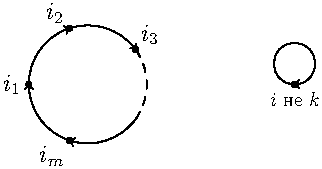
\includegraphics[width=5cm]{image/lecture-16.pdf}
    \end{matrix}$
  \end{definition} 
  \begin{example1}
    $n=6, \ \ \sigma=(1,3,2)$
    $\begin{matrix}\tab[1cm]
      % \begin{asy}
      %   % \usepackage[russian]{babel};
      %   texpreamble("\usepackage[T2A]{fontenc}\usepackage[utf8]{inputenc}
      %   \usepackage{mathtext}\usepackage[russian]{babel}");
      %   unitsize(0.48cm);
      %   pair i1 = (-1, 0), O = (0, 0);
      %   transform r=rotate(-120,O);
      %   transform r2=rotate(120,O);
      %   dot("$1$",i1, W);
      %   dot("$2$",r*i1, NE);
      %   dot("$3$",r*(r*i1), SE);

      %   path p1=r*i1{dir(rotate(90)*(r*i1-O))}..i1;
      %   draw(p1,Arrow(TeXHead));

      %   path p2=r*(r*i1){dir(rotate(90)*(r*(r*i1)-O))}..r*i1;
      %   draw(p2,Arrow(TeXHead));

      %   path p3=i1{dir(rotate(90)*(i1-O))}..r2*i1;
      %   draw(p3,Arrow(TeXHead));


      %   pair a1 = (3, 0), b1 = (3, 0.7);
      %   pair a2 = (5, 0), b2 = (5, 0.7);
      %   pair a3 = (7, 0), b3 = (7, 0.7);

      %   dot(scale(0.8)*Label("$4$"),a1, S);
      %   dot(scale(0.8)*Label("$5$"),a2, S);
      %   dot(scale(0.8)*Label("$6$"),a3, S);

      %   path p4=a1{dir(rotate(90)*(a1-(3, 0.35)))}..b1;
      %   path p5=b1{dir(rotate(90)*(b1-(3, 0.35)))}..a1;
      %   draw(p4);
      %   draw(p5,Arrow(TeXHead));

      %   path p6=a2{dir(rotate(90)*(a2-(5, 0.35)))}..b2;
      %   path p7=b2{dir(rotate(90)*(b2-(5, 0.35)))}..a2;
      %   draw(p6);
      %   draw(p7,Arrow(TeXHead));

      %   path p8=a3{dir(rotate(90)*(a3-(7, 0.35)))}..b3;
      %   path p9=b3{dir(rotate(90)*(b3-(7, 0.35)))}..a3;
      %   draw(p8);
      %   draw(p9,Arrow(TeXHead));
      % \end{asy}
      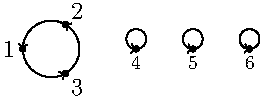
\includegraphics[width=4.5cm]{image/lecture-17.pdf}
    \end{matrix}$
  \end{example1}
\begin{remark}
  Заметим, что $(i_1,i_2,...,i_k) = (i_k,i_1,...,i_{k-1}) = (i_2,i_3,..,i_1) = ...$ 
\end{remark} 
\begin{definition}
  Циклы $(i_1,...,i_k)$ и $(j_1,...,j_k)$ называются независимыми, если: $$\{i_1,...,i_k\} \cap \{j_1,...,j_k\} = \varnothing $$  
\end{definition} 
\begin{example1}
  $(1,2,3), \ (4,5)$ 
\end{example1}
\begin{subtheorem}
  Независимые циклы коммутируют.
\end{subtheorem} 
\begin{example1}
  $\begin{pmatrix}
    1 & 2 & 3 & 4 & 5 & 6 \\
    2 & 3 & 1 & 5 & 4 & 6
  \end{pmatrix} = \begin{pmatrix}
    1 & 2 & 3
  \end{pmatrix} \begin{pmatrix}
    4 & 5
  \end{pmatrix} \begin{pmatrix}
    6
  \end{pmatrix}$
  
\end{example1}
\setcounter{thcount}{0}
\begin{theoremnum} 
  Любая подстановка $\sigma \in S_n,\ \sigma \neq \textrm{id}$ раскладывается в произведение $\text{\underline{независимых} }$ циклов длины $\geq 2$, причем это разложение единственно с точностью до перестановки множителей. \label{1pum}
\end{theoremnum}
\begin{proof} \tab
  \begin{itemize}
    \item[ $\exists$: ] Рассмотрим степени подстановки $\sigma$. \\
    По определению: $\sigma^0 = \textrm{id};$ \\ 
    \tab[3.80cm] $\sigma^m := \sigma \cdot ... \cdot \sigma, $ при $m>0;$\\
    \tab[3.80cm] $\sigma^m := \sigma^{-1} \cdot ...\cdot \sigma^{-1}$, при $m<0$ \\
    Отметим, что: \begin{enumerate}
      \item Степень подстановки $\sigma^m$ - это подстановка $\forall m \in \Z$
      \item $\sigma^{m_1}\cdot \sigma^{m_2} = \sigma^{m_1+m_2}$
      \item $(\sigma^{m_1})^{m_2} = \sigma^{m_1 \cdot m_2}$  
    \end{enumerate}
    Рассмотрим произвольный $i \in \{1,...,n\}$
    \begin{center}
      % \begin{asy}
      %   unitsize(1.5cm);
      %   pair [] i;
      %   i[0] = (0, 0); i[1] = (1, 0); i[2] = (2, 0); i[3] = (3, 0); i[4] = (4, 0); i[5] = (5, 0); i[6] = (6, 0);
      %   dot("$\sigma^{-1}(i)$", i[1], S);
      %   dot("$i$", i[2], S);
      %   dot("$\sigma(i)$", i[3], S);
      %   dot("$\sigma^{2}(i)$", i[4], S);

      %   path p1=i[0]{dir(rotate(-131)*(i[0]-((i[1]-i[0])/2+i[0])))}..i[1];
      %   draw(p1,Arrow(TeXHead));

      %   path p2=i[1]{dir(rotate(-131)*(i[1]-((i[2]-i[1])/2+i[1])))}..i[2];
      %   draw(p2,Arrow(TeXHead));
      %   draw(Label("$\sigma$"),p2, N);

      %   path p3=i[2]{dir(rotate(-131)*(i[2]-((i[3]-i[2])/2+i[2])))}..i[3];
      %   draw(p3,Arrow(TeXHead));
      %   draw(Label("$\sigma$"),p3, N);

      %   path p4=i[3]{dir(rotate(-131)*(i[3]-((i[4]-i[3])/2+i[3])))}..i[4];
      %   draw(p4,Arrow(TeXHead));
      %   draw(Label("$\sigma$"),p4, N);

      %   path p5=i[4]{dir(rotate(-131)*(i[4]-((i[5]-i[4])/2+i[4])))}..i[5];
      %   draw(p5,Arrow(TeXHead));
      %   draw(Label("$\sigma$"),p5, N);
      % \end{asy}
      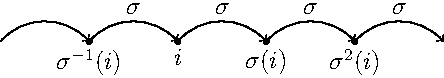
\includegraphics[width=7cm]{image/lecture-18.pdf}
    \end{center}
    \begin{definition}
      Множество $\textrm{Orb}(i) = \{\sigma^m(i) \ | \ m \in \Z\}$  называется орбитой числа $i$.
    \end{definition} 
     $\textrm{Orb}(i) \subseteq \{1,...,n\} \Longrightarrow \exists \ m_1,m_2 \in \Z: \sigma^{m_1}(i) = \sigma^{m_2}(i)$ \\
     Допустим, что $m_1 > m_2$, тогда $\sigma^{m_1 - m_2}(i)=j \\
     \Longrightarrow $ (т.к. $m_1 - m_2 \in \N)$ $\exists \ $ такое наименьшее $k \in \N^0 \ : \ \sigma^k(i)= j$ 
    $$\textrm{Orb}(i) = \{i, \sigma(i),...,\sigma^{k-1}(i)\}$$.
    \begin{properties} \tab
      \begin{enumerate}
        \item Различные орбиты не пересекаются. 
        \begin{proof}
          Пусть $l \in \textrm{Orb}(i) \cap \textrm{Orb}(j) \Longrightarrow \exists \ m_1, m_2 \in \N^0 : \\
        \sigma^{m_1}(i) = l = \sigma^{m_2}(j) \Longrightarrow \sigma^{m_1-m_2}(i) = j \Longrightarrow \\ \forall m \in \Z: \ 
        \sigma^{m}(j)= \sigma^{m(m_1-m_2)}(i) \Longrightarrow \textrm{Orb}(j) \subseteq  \textrm{Orb}(i)$ \\
        Аналогично $\textrm{Orb}(i) \subseteq \textrm{Orb}(j) \Longrightarrow \textrm{Orb}(i) = \textrm{Orb}(j)$
        \end{proof} 
        \item $\{1,...,n\} = \textrm{Orb}(i_1) \cup ... \cup \textrm{Orb}(i_s)$ 
        \begin{proof}
          Т.к. $\forall i \in \{1,...,n\}: \ i \in \textrm{Orb}(i)$ 
        \end{proof} 
      \end{enumerate}
    \end{properties}
    $\{1,...,n\} = \underset{k_1}{\textrm{Orb}(i_1)} \sqcup ... \sqcup \underset{k_t}{\textrm{Orb}(i_t)}\sqcup \underset{k_{t+1}}{\textrm{Orb}(i_{t+1})} \sqcup ... \sqcup \underset{k_s}{\textrm{Orb}(i_s)}$ \\ $\\$ 
    Если $\sigma \neq \textrm{id}$, то $k_1>1,...,k_t>1,k_{t+1}=1,...,k_s=1 \Longrightarrow \\
    \sigma = (i_1 \ \sigma(i_1) \ ... \ \sigma^{k_1-1}(i_1)) \ ... \ (i_t \ \sigma(i_t) \ ... \ \sigma^{k_t-1}(i_t))$. $\exists$ \ доказано.   
    \item[ $!:$ ](От противного)\\
    Допустим, $$\sigma = \pi_1,...,\pi_{\nu}$$ $$\sigma = \tau_1,...,\tau_{\mu}$$  Различные разложения на независимые циклы длины $\geq 2$ \\
    Т.к. $\sigma \neq id$, то $\exists \ j: \sigma(j) \neq j \Longrightarrow $ с точностью до нумерации $$\pi_1(j) \neq j, \ \tau_1(j) \neq j$$  
    $$\begin{matrix}
      \sigma(j) = \pi_1(j) \\
      \sigma(j) = \tau_1(j)
    \end{matrix} \ \Longrightarrow \forall m \in \Z  \ \ \begin{matrix}
      \sigma^m(j) = \pi_1^m(j) \\
      \sigma^m(j) = \tau_1^m(j)
    \end{matrix}$$ 
    Т.к. цикл полностью определяется степенями $\sigma$, то $\pi_1 = \tau_1 \Longrightarrow \pi_2 ... \pi_{\nu} = \tau_2 ... \tau_{\mu}$. Далее индукция по $\nu$ и $\mu \Longrightarrow $ Противоречие $\Longrightarrow $ Разложение $\sigma$ единственно.   
    \end{itemize}
  \end{proof} 
  \begin{definition}
    Цикл длины 2 называется транспозицией. 
  \end{definition}
  \begin{theorem}
    Любая подстановка $\sigma \in S_n$ раскладывается в произведение транспозиций. 
  \end{theorem} 
  \begin{proof}
    Если $\sigma = \textrm{id}$, то $\sigma = (12)(12)$ \\
    Если $\sigma \neq \textrm{id}$, то по Теореме \eqref{1pum} $\sigma$ раскладывается в произведение независимых циклов длины $\geq 2$ \\
    Поэтому достаточно разложить на транспозиции каждый такой цикл.
    $$k>1 \ \ \ (1,2,...,k) = (1,k)(1,k-1)...(1,3)(1,2)$$     
  \end{proof} 
  \subsection{Четность подстановки}
  $\sigma \in S_n$; \ \ $\sigma = \begin{pmatrix}
    i_1 & \cdots & i_n \\
    j_1 & \cdots & j_n
  \end{pmatrix}$  
  \begin{definition}
    Знаком подстановки $\sigma$ называется функция: 
    $$\textrm{sgn} (\sigma):= \textrm{sgn}(i_1,...,i_n)\cdot \textrm{sgn}(j_1,...,j_n)$$  
  \end{definition} 
  \begin{subtheorem}
    Знак подстановки не зависит от способа записи подстановки в виде таблицы.
  \end{subtheorem} 
  \begin{proof}
    Если $\begin{pmatrix}
    i_1 & \cdots & i_n \\
    j_1 & \cdots & j_n
  \end{pmatrix}$ и $\begin{pmatrix}
    m_1 & \cdots & m_n \\
    k_1 & \cdots & k_n
  \end{pmatrix}$ - две записи одной и той же подстановки $\sigma$, то от $\begin{pmatrix}
    i_1 & \cdots & i_n \\
    j_1 & \cdots & j_n
  \end{pmatrix}$ к $\begin{pmatrix}
    m_1 & \cdots & m_n \\
    k_1 & \cdots & k_n
  \end{pmatrix}$ можно перейти за конечное число перемен столбцов местами. Каждая перемена столбцов местами производит транспозицию в верхней и в нижней строке $\Longrightarrow $ знак меняется и там, и там $\Longrightarrow $ знак произведения не изменяется. 
  \end{proof} 
  В стандартной записи $\sigma = \begin{pmatrix}
    1 & 2 & \cdots & n \\
    i_1 & i_2 & \cdots & i_n
  \end{pmatrix} \Longrightarrow \textrm{sgn} (\sigma) = \textrm{sgn} (i_1,i_2,...,i_n)$  
  \begin{definition}
    Подстановка $\sigma$ называется четной (нечетной), если: 
    $$\textrm{sgn} (\sigma) = 1 \ \ (\textrm{sgn} (\sigma) = -1)$$  
  \end{definition} 
  \begin{properties} \tab 
    \begin{enumerate}
      \item $\textrm{sgn} (\sigma^{-1}) = \textrm{sgn} (\sigma)$
      \begin{proof}
        $\sigma = \begin{pmatrix}
          i_1 & \cdots & i_n \\
          j_1 & \cdots & j_n
        \end{pmatrix} \Longrightarrow \sigma^{-1} = \begin{pmatrix}
          j_1 & \cdots & j_n \\
          i_1 & \cdots & i_n  
        \end{pmatrix}$ 
      \end{proof}
      \item \label{propertie2} $\textrm{sgn} (\sigma \cdot \tau) = \textrm{sgn}(\sigma) \cdot \textrm{sgn}(\tau) \ \ (\sigma, \tau \in S_n)$ 
      \begin{proof}
        $$\sigma = \begin{pmatrix}
          i_1 & \cdots & i_n \\
          j_1 & \cdots & j_n
        \end{pmatrix}, 
        \tau = \begin{pmatrix}
        k_1 & \cdots & k_n \\
        i_1 & \cdots & i_n
        \end{pmatrix} $$ $ \Longrightarrow \sigma \cdot \tau = \begin{pmatrix}
          k_1 & \cdots & k_n \\
          j_1 & \cdots & j_n
        \end{pmatrix} \Longrightarrow \textrm{sgn}(\sigma \cdot \tau) = \textrm{sgn}(k_1,...,k_n) \cdot \textrm{sgn}(j_1,...,j_n) = \textrm{sgn}(k_1,...,k_n) \cdot \underbrace{\textrm{sgn}(i_1,....,i_n) \cdot \textrm{sgn}(i_1,....,i_n)}_{1}   \cdot \textrm{sgn} (j_1,...,j_n) = \textrm{sgn}(\sigma) \cdot \textrm{sgn} (\tau)$ 
      \end{proof} 
    \end{enumerate}
  \end{properties}
  \begin{subtheorem}\tab
    \begin{enumerate}
      \item \label{Ytv1} если $\tau$ - транспозиция, то $\textrm{sgn}(\tau) = -1$
      \item если $\sigma$ - цикл длины $k$, то $\textrm{sgn}(\sigma) = (-1)^{k-1}$
      \item \label{Ytv3}если $\sigma = \tau_1 \cdot ... \cdot \tau_l$, где $\tau_i$ - транспозиции, то $\textrm{sgn}(\sigma) = (-1)^l$      
    \end{enumerate}
  \end{subtheorem}
  \begin{proof}\tab
    \begin{itemize}
      \item[1)] $$\tau = \begin{pmatrix}
        1 & \cdots & i & \cdots & j & \cdots n \\
        1 & \cdots & j & \cdots & i & \cdots n
      \end{pmatrix} $$$  \Longrightarrow \textrm{sgn} (\tau) = \textrm{sgn}(1,...,j,...,i,...,n) = \textrm{sgn}(1,...,i,...,j,...,n) = -1$  
      \item[3)] следует из Свойства \eqref{propertie2} и Утверждения \eqref{Ytv1}:
      $$\textrm{sgn}(\sigma) = \textrm{sgn}(\tau_1) \cdot \textrm{sgn}(\tau_2) \cdot ... \cdot \textrm{sgn}(\tau_l) = \underbrace{(-1)\cdot(-1)\cdot ... \cdot(-1)}_{l} = (-1)^{l}$$ 
      \item[2)] $\sigma = (i_1,...,i_k) = (i_1,i_k)(i_1,i_{k-1})...(i_1,i_2) =$ (по Утверждения \eqref{Ytv3}) $= (-1)^{k-1}$ 
    \end{itemize}
  \end{proof}
  \begin{example1}
    $$\begin{pmatrix}
      1 & 2 & 3 & 4 & 5 & 6 \\
      3 & 1 & 2 & 5 & 4 & 6
    \end{pmatrix} = \begin{pmatrix}
      1 & 3 & 2
    \end{pmatrix} \begin{pmatrix}
      4 & 5 
    \end{pmatrix} = (-1)^2 \cdot \text{ (нечет) }=$$
    $$ = \text{ (чет) }\cdot \text{ (нечет) } = \text{ (нечет) }$$
  \end{example1}
  \subsection{Подгруппа}
  $(A,*)$ - множество с бинарной операцией. \ $B \subseteq A$ 
  \begin{definition}
    Говорят, что $B$ замкнуто относительно бинарной опериции $*$, если: $$\forall b_1,b_2 \in B: \ b_1 * b_2 \in B$$
    В этом случае $B$ превращается в алгебраическую структуру.   
  \end{definition}  
  \begin{example1}
    $\N \text{ (коммутативная полугруппа) }  \subset \Z \text{ (с + абелева группа) }$ 
  \end{example1}
  \begin{definition}
    Множество $H$ называется подгруппой группы $G$, если:
    \begin{enumerate}
      \item $\forall h_1,h_2 \in H \Longrightarrow h_1 \cdot h_2 \in H$ 
      \item $1 \in H$
      \item $\forall h \in H \Longrightarrow h^{-1} \in H$  
    \end{enumerate}
    Обозначается: $H\leq G$ 
  \end{definition} 
  \begin{subtheorem}
    Любая подгруппа группы $G$ сама является группой, относительно той же операции.
  \end{subtheorem} 
  \begin{remark}
    В определении подгруппы $(2.) \longleftrightarrow "H \neq \varnothing"$ 
  \end{remark} 
  \begin{example}\tab
    \begin{itemize}
      \item[1)] $\N\leq \Z$
      \item[2)] $\Z \leq \Q \leq \R$
      \item[3)] $m\Z \leq\Z, \ m\in \N$   
      \item[4)] $A_n$ - все четные подстановки\\
      $A_n \leq S_n$. (для нечетных неверно)    
    \end{itemize}
  \end{example}
  \subsection{Кольца и поля}
  \begin{definition}
    Множество $K$, на котором введены 2 бинарные операции:\\ $"+"$ - сложение, $"\cdot"$ - умножение, называется кольцом, если выполнены следующие аксиомы:
    \begin{enumerate}
      \item $(K, +)$ - абелева группа
      \item $\forall a,b,c \in K: \ a(b+c) = ab+ac$ и $(a+b)c = ac+ab$   
    \end{enumerate}
    Обозначается: $(K, +, \cdot)$
  \end{definition} 
  \begin{example}\tab
    \begin{enumerate}
      \item $(\Z, +, \cdot)$
      \item $(M_n(\R), +, \cdot)$
    \end{enumerate}
  \end{example}
  \begin{definition}
    Кольцо называется ассоциативным, если умножение ассоциативно.
  \end{definition}
  \begin{definition}
    Кольцо называется коммутативным, если умножение коммутативное.
  \end{definition}
  \begin{definition}
    Кольцо называется кольцом с единицей, если существует нейтральный элемент по умножению:
    $$\exists \ 1 \in K: \ \forall a\in K: \ 1 \cdot a = a \cdot 1 = a$$ 
  \end{definition}
  \begin{subtheorem}
    Если в $K$ есть единица, то она единственная. 
  \end{subtheorem} 
  \begin{example} \tab
    \begin{enumerate}
      \item $(\Z, +, \cdot)$ - коммутативное, ассоциативное кольцо с 1
      \item $(M_n(\R), +, \cdot)$ - НЕ коммутативное, ассоциативное кольцо с 1
      \item $(V^3,+, x)$, ($x$ - векторное произведение) - НЕ коммутативное, НЕ ассоциативное кольцо без 1
      \item $(2\Z, +, \cdot)$ -  коммутативное, ассоциативное кольцо без 1
    \end{enumerate}
  \end{example}
  \begin{consequenses} \textbf{(простейшие)} 
    \begin{enumerate}
      \item \begin{itemize}
        \item $0$ - единственный
        \item $\forall a\in K$ - противоположный единственный
        \item $\forall a, b\in K \ \exists! \ x \in K: \ a+x=b$ $\Longrightarrow  x = b+(-a)$; \  ($x \ !,$ т.к. $(-a) \ !$) \\   
        Обозначается: $x = b-a$ 
      \end{itemize}
      \item $\forall a \in K: \ a \cdot 0=0 \cdot a = 0$
      \item $a\cdot(-b) = (-a)\cdot b = -(a\cdot b)$  
      \item $\forall a, b, c \in K: \ a(b-c) = ab-ac, \ (b-c)a = ba-ca$ 
      \item Если $K$ - кольцо с 1, то $a(-1) = (-1)a = -a$ 
    \end{enumerate}
  \end{consequenses}
  \begin{remark}
    Пусть $K$ - кольцо с единицей (1), тогда если $0 = (1) \Longrightarrow K = \{0\}$ 
  \end{remark}
  \begin{proof}
    $\forall a \in K: \ 0 = 0 \cdot a= 1 \cdot a \Longrightarrow a = 0$ 
  \end{proof} 
  Пусть $K$ - кольцо с единицей 
  \begin{definition}
      Элемент $a \in K$ называется обратимым, если: $$\exists \ b \in K: ab =ba = 1$$ 
      При этом элемент $b$ должен быть обратным к $a$   
  \end{definition}  
  \begin{subtheorem}
    Пусть $K$ - ассоциативное кольцо с 1, тогда если элемент $a \in K$ имеет обратный, то он единственный.  
  \end{subtheorem} 
  \begin{example} \tab
    \begin{enumerate}
      \item $(\Z, +, \cdot)$: \  $1, -1$ - обратимые, других нет.
      \item $(\R, +, \cdot)$: \ $\forall a \in \R, \ a \neq 0$ - обратим. \\
      Обозначается: $K$ - ассоциативное кольцо с 1  
    \end{enumerate}
  \end{example}
  $K^*$ - множество элементов кольца $K$, имеющих обратный. 
  \begin{subtheorem}
    $K^*$ - группа относительно умножения. 
  \end{subtheorem}  
  \begin{example1}
    $\Z^* = \{1, -1\}$
  \end{example1}
  \begin{definition}
    Поле $K$ - коммутативное, ассоциативное кольцо с $1 \neq 0$ , в котором любой ненулевой элемент обратим.
  \end{definition} 
  \begin{remark}
    $0 = (1) \Longleftrightarrow K = \{0\}$ - не поле.
  \end{remark} 
  \begin{example}\tab
    \begin{enumerate}
      \item $(\R, +, \cdot)$ - поле
      \item $(\Q, +, \cdot)$ - поле
      \item $(\Z, +, \cdot)$ - НЕ поле   
    \end{enumerate}
  \end{example}
  \begin{example1}
    $\Z_n$ - коммутативное, ассоциативное кольцо с 1
  \end{example1}
  \begin{subtheorem}
    $k \in \Z_n$ - обратим $\Longleftrightarrow (k, n) = 1$  
  \end{subtheorem} 
  \begin{theorem}
    $\Z_n$ - поле $\Longleftrightarrow n - $ простое 
  \end{theorem} 
  \begin{proof}\tab
    \begin{itemize}
      \item[$\underline{\Longrightarrow}$] Пусть $\Z_n$ - поле, тогда $\forall k \in \Z_n$ имеет обратный $m : \ km=1$.\\ Предположим, что $n$ - не простое, тогда $n = st, $ где $1<s, t<n \\ \Longrightarrow s \neq 0$ в $\Z_n$
      $\Longrightarrow s $ имеет обратный $\widetilde{s} : \ s \cdot \widetilde{s} = 1$ в $\Z_n$\\
      $\Longrightarrow t \cdot s \cdot \widetilde{s} = t $ в $
      \Z_n \Longrightarrow t=0$ в $\Z_n$ - противоречие.
      \item[$\underline{\Longleftarrow}$] $n$ - простое, то $\forall k \in \Z_n: \ k \neq 0$ в $\Z_n$, т.е. $n \neq k \Longrightarrow (n, k) = 1 \\ \Longrightarrow k$ - обратим.  
    \end{itemize}
  \end{proof}
  \begin{definition}
    Говорят, что кольцо $K$ не имеет делителей нуля, если из равенства $a \cdot b =0 \Longrightarrow a = 0 $ или $b=0$.\\
    Если же для ненулевого элемента $a \in K$ найдется  ненулевой элемент $b  \in K: \ a \cdot b = 0, $ то $a, b $ называются делителями нуля.
  \end{definition} 
  \begin{example} \tab
    \begin{enumerate}
      \item $\Z:$ без делителя нуля 
      \item $\Z_6: \ 2 \cdot 3 =0 \Longrightarrow $ есть делители нуля.  
      \item $M_2(\R)$: \ $\begin{pmatrix}
        1 & 0 \\ 0 & 0
      \end{pmatrix} \cdot \begin{pmatrix}
        0 & 0 \\ 0 & 1
      \end{pmatrix} = \begin{pmatrix}
        0 & 0 \\ 0 & 0 
      \end{pmatrix}$ 
    \end{enumerate}
  \end{example}
  \begin{subtheorem}
    Если в кольце $K$ нет делителя нуля, то возможно сокращение, если $a \cdot c = b \cdot c, $ и $c \neq 0, $ то $a = b$  
  \end{subtheorem}
  \begin{proof}
    $a \cdot c = b \cdot c \Longrightarrow a \cdot c - b \cdot c =0 \Longrightarrow (a-b) \cdot c =0$\\
    т.к. нет делителя нуля $\Longrightarrow $ либо $c=0$, либо $a-b=0, $ но $c \neq 0 \Longrightarrow a=b$   
  \end{proof}  
  \begin{subtheorem}
    В поле нет делителя нуля.
  \end{subtheorem} 
  \begin{proof}
    Предположим, что:
    $\begin{cases}
      a \cdot b =0\\a \neq 0 \\ b \neq 0
    \end{cases}$ т.к. $a \neq 0$, в поле $\exists \ a^{-1}$\\
    Умножим $a \cdot b =0 $ на $a^{-1}$ \\ $\\$ 
    $\begin{cases}
      a^{-1}(a \cdot b) = a^{-1} \cdot 0 = 0\\
      a^{-1}(a \cdot b) = (a^{-1} \cdot a)b = 1 \cdot b =b
    \end{cases}$ $ \Longrightarrow b =0$
  \end{proof} 
  \begin{subtheorem}
    Пусть $K$ - коммутативное, ассоциативное кольцо с 1, тогда: $$x - \text{обратный} \Longleftrightarrow x - \text{не делитель нуля}$$  
  \end{subtheorem} 
  \begin{proof}
    Упражнение
  \end{proof}
  \subsection{Изоморфные кольца и поля}
  \begin{definition}
    Кольца $K$ и $\widetilde{K}$ называются изоморфными, если: 
    $\exists \ \phi: \ K \to \widetilde{K}:$
    \begin{enumerate}
      \item $\phi$ - биекция
      \item $\forall a, b \in K: \ \phi(a+b) = \phi(a)+\phi(b)$
      \item $\forall a, b \in K: \ \phi(ab) = \phi(a)\cdot \phi(b)$ 
    \end{enumerate}
    Обозначается: $K\cong \widetilde{K}$, \ $\phi \ - $ изоморфизм колец 
  \end{definition} 
  \begin{consequenses}\tab
    \begin{enumerate}
      \item $\phi(0) = \widetilde{0}$
      \item $\phi(-a) = -\phi(a)$
      \item Если $K$ - ассоциативное кольцо с 1, то $\phi(1) = 1$, \\а если $a \in K$ имеет обратный, то $\phi(a^{-1}) = \phi(a)^{-1}$
    \end{enumerate}
  \end{consequenses} 
  \begin{definition}
    Поля $P$ и $\widetilde{P}$  изоморфны, если они изоморфны как кольца.
  \end{definition} 
  \begin{definition}
    Подмножество $L$ кольца $K$ называется подкольцом, если:
    \begin{enumerate}
      \item $L$ - подгруппа адитивной группы кольца $K$, т.е.
      \begin{itemize}
        \item $\forall a, b \subset L : \ a + b \in L$ 
        \item $0 \in L$ 
        \item $\forall a \in L: (-a) \in L$
      \end{itemize}
      \item $\forall a, b \in L: \ a \cdot b \in L$    
    \end{enumerate}
  \end{definition} 
  \begin{subtheorem}
    Любое подкольцо кольца $K$ само является кольцом относительно тех же операций.  
  \end{subtheorem}
  \begin{definition}
    Подмножество $L$ поля $K$ называется подполем, если:
    \begin{enumerate}
      \item $L$ - подкольцо кольца $K$
      \item $1 \in L$
      \item $\forall a \in L, \ a \neq 0 \Longrightarrow a^{-1} \in L$   
    \end{enumerate}
  \end{definition}
  \begin{subtheorem}
    Любое подмножество поля $K$ само является полем относильно тех же операций.  
  \end{subtheorem}  
  \begin{example} \tab
    \begin{enumerate}
      \item $\Q \subseteq \R$ - подполе
      \item $\Z \subseteq \R$ - подкольцо
      \item $2\Z \subseteq \Z$ - подкольцо
    \end{enumerate}
  \end{example} 
  \begin{Exercise}
    В $\Q$ нет подполей, отличных от самого $\Q$.
  \end{Exercise}
  \subsection{Характеристика поля}
  \begin{definition}
    Говорят, что поле $P$ имеет характеристику $n$, если $n$ - наименьшее натуральное число, такое, что $\underbrace{1 + 1 + ... + 1}_{n} = 0 $. \\
    Если такого числа нет, то говорят, что поле имеет характеристику 0.\\
    Обозначается: $\textrm{char}P=n$ 
  \end{definition} 
  \begin{example} \tab
    \begin{enumerate}
      \item $\textrm{char}\Z_3 = 3 \ (1 + 1 + 1 = 0)$
      \item $\textrm{char}\R = 0$  
    \end{enumerate}
  \end{example}
  \begin{remark}
    Если $n \neq 0, \ \textrm{char}P = n, $ то $\forall a \in P:$ 
    $$ \underbrace{a+a+...+a}_{n} = \underbrace{a\cdot 1+a\cdot 1+...+a\cdot 1}_{n} = a\cdot (\underbrace{1+1+...+1}_{n}) = a \cdot 0 =0 $$ 
  \end{remark} 
  \begin{subtheorem}
    Если $P$ - поле характеристики $n$, \ $n \neq 0$, то $n \ -$ простое. 
  \end{subtheorem} 
  \begin{proof}
    Докажем, $n=m\cdot k, \ 1<m, \ k<n$:
    $$\underbrace{1+1+...+1}_{n} = (\underbrace{1+1+...+1}_{m})(\underbrace{1+1+...+1}_{k})\Longrightarrow m \cdot k=0$$  
    В поле нет делителей нуля $\Longrightarrow \underbrace{1+1+...+1}_{m} = 0$. Противоречие.
  \end{proof}
  \begin{remark}
    Теория решения СЛУ (метод Гаусса, правила Крамера, ...), теория определителей, утверждения о векторных пространсвах (в частности о матрицах), которые мы рассматривали раннее, переносятся с $\R$ на произвольные поля. \\
    \textbf{Исключение}  - поле характеристики 2: в определении кососимметричной и полилинейной функции надо требовать, чтобы при 2 совпадающих аргументах \\ $f(...,v,...,v,...)=0$. Отсюда получаем, что $f(...,v,...,w,...) = -f(...,w,...,v,...)$ (при $\textrm{char}P = 2$ получаем: $1 = -1$)  
  \end{remark}
  \subsection{Поле комплексных чисел}
  % $$\textbf{xd}$$ 
  \begin{definition}
    Поле комплексных чисел $\mathbb{C} $ - это поле, в котором выполнены следующие условия:
    \begin{enumerate}
      \item Поле $\R$ содержится в $\mathbb{C} $ в качестве подполя.
      \item В $\mathbb{C} \ \exists$ элемент $i:\  i^2 = -1$
      \item $\mathbb{C} $ - наименьшее поле, удовлетворяющее условиям 1. и 2.     
    \end{enumerate}
    Т.е. $\forall F\subseteq \mathbb{C}: \ \R \subseteq F, \ i\in F \Longrightarrow  F = \mathbb{C}$ 
  \end{definition} 
  \begin{theorem}
    Поле $\mathbb{C}$ комплексных чисел существует, причем оно единсвенно с точностью до изоморфизма, оставляющего все вещественные числа на месте. Кроме того, $\forall z \in \mathbb{C}$ представляется единсвенным образом в виде: $z = a + bi$, где $a, b \in \R$.
  \end{theorem} 
  \begin{proof}\tab
    \begin{itemize}
      \item[1.)]Предположим, что поле комплексных чисел $\mathbb{C}$ существует, и докажем его единственность. \\
      Для этого исследуем $\mathbb{C}$ \\
      Рассмотрим в $\mathbb{C}$ подмножество $$F = \{a+bi \ | \ a,b \in \R\} \subseteq \mathbb{C}$$
      Докажем, что $F$ - подполе:
      $$(a+bi) + (\widetilde{a}+\widetilde{b}i) = (a + \widetilde{a})+(b+\widetilde{b})i \in F$$ 
      $$(a+bi)(\widetilde{a}+\widetilde{b}i) = (a \widetilde{a}-b \widetilde{b}) + (a \widetilde{b}+ \widetilde{a} b)i \in F$$ 
      \begin{itemize}
        \item[$\circ$] $0 = 0 + 0i \in F$
        \item[$\circ$] $1 = 1 + 0i \in F$
        \item[$\circ$] $-(a+bi) = (-a) + (-b)i\in F$  
        \item[$\circ$] $\forall a+bi \in F$ будем искать обратный в виде: $$x+yi: (a+bi)(x+yi)= (a x-b y) + (a y+ x b)$$  
        $\begin{cases}
          ax - by =1\\
          ay+bx=0
        \end{cases}$
      \end{itemize}
      \begin{itemize}
        \item[1 случай.] $b \neq 0: \ \begin{cases}
          -\frac{a^2y}{b} - by =1\\
          x = -\frac{ay}{b}
        \end{cases}$
        Т.к. $a+bi \neq 0 \Longrightarrow a^2+b^2 \neq 0$ \\ $\\$ 
        $\Longrightarrow \exists \ y = -\frac{b}{a^2 + b^2}, \ x = \frac{a}{a^2 + b^2} \in \R$ 
        \item[2 случай.] homework
      \end{itemize}
      $\Longrightarrow F$ - подполе поля $\mathbb{C}$ \\
      $\R \subseteq F$, т.к. $i =0 + 1 \cdot i \in F$\\
      По третьей аксиоме из определения поле $\mathbb{C}: \ F=\mathbb{C}$\\
      Мы доказали, что если поле помплексных чисел существует, то любой элемент в нем представляется в виде $z = a =bi$, где $a, b \in \R$.\\
      Проверим, что это представление единственное. \\
      От противного: 
      $$a+bi = \widetilde{a} + \widetilde{b}, \ \ a, \widetilde{a}, b, \widetilde{b} \in \R$$ 
      $$a - \widetilde{a} = (\widetilde{b}-b)i$$
      $$(a-\widetilde{a})^2 = -1 (\widetilde{b}-b) - \text{ это вещественное число}$$ 
      $$\begin{cases}
        (a-\widetilde{a})^2\geq 0\\
        (\widetilde{b}-b)^2\geq 0 
      \end{cases} \Longrightarrow \begin{cases}
        (a-\widetilde{a})^2 =0\\
        (\widetilde{b}-b)^2 =0
      \end{cases} \Longrightarrow  \begin{cases}
        a=\widetilde{a} \\
        b = \widetilde{b}
      \end{cases}$$ $\\$ 
      Предположим, что есть еще одно поле комплексных чисел $\mathbb{C}$. \\
      Т.к. рассуждения выше верны и для $\mathbb{C}$, то $\forall \widetilde{z} \in \widetilde{\mathbb{C}}$ представляетя единственным образом в виде: 
      $$\widetilde{z} = a+b\widetilde{i}, \text{ где } a, b \in \R, \ (\widetilde{i})^2 = -1$$
      Рассомтрим отображение: 
      $$\phi: \mathbb{C} \to \widetilde{\mathbb{C}}$$
      $$\phi: a+bi \to a+ b \widetilde{i}$$
      Это отображение - изоморфизм полей, сохраняющий вещественные числа на месте.
      \item[2.)]Докажем существование поля помплексных чисел. \\
      Построим поле, удовлетворяющее определению:
      $$\Gamma = \{(a, b) \ | \ a, b \in \R\}$$
      Введем операции:
      \begin{itemize}
        \item[$\circ  $ ] $(a, b) + (\widetilde{a}, \widetilde{b}) = (a+\widetilde{a}, b + \widetilde{b})$
        \item[ $\circ   $ ] $(a, b)(\widetilde{a}, \widetilde{b}) = (a\widetilde{a} - b \widetilde{b}, a \widetilde{b} + \widetilde{a}b)$
      \end{itemize}
      \begin{enumerate}
        \item Это бинарная операция; Выполнены коммутативность,\\ ассоциативность, дистрибутивность (непосредственная проверка).
        \item $(0,0)$ - ноль
        \item $(-a, -b)$ - противоположный к $(a, b)$
        \item $(1, 0)$ - единица
        \item $\forall (a, b) \neq (0, 0) \ \exists \ \text{ обратный }: (\frac{a}{a^2+b^2}, \frac{-b}{a^2+b^2})$
      \end{enumerate} $\Longrightarrow \Gamma$ - поле.\\
      Рассмотрим подмножество $\mathsf{L} \subseteq \Gamma: $  
      $$\mathsf{L}  = \{(a, 0) \ | \ a \in \R \}$$   
      Это поле изоморфное $\R:$
      \begin{itemize}
        \item[$\circ$] $a\longleftrightarrow (a, 0)$
        \item[$\circ$] $-1 \longleftrightarrow (-1, 0) = (0, 1)(0, 1)$
        \item[$\circ$] $i = (0, 1) \in \Gamma$
        \item[$\circ$] $\forall (a, b) \in \Gamma: $
        $$(a, 0)(1, 0) + (b, 0)(0, 1) = (a, b)$$
        т.е. $\forall z \in \Gamma:$ 
        $$z = a \cdot 1 + b \cdot i$$
      \end{itemize}
      $\forall F \subseteq \Gamma: \ $
         $\begin{cases}
        \R \subseteq F \\
        i \in F
      \end{cases} \Longrightarrow F = \Gamma$
    \end{itemize}
  \end{proof} 
  \begin{remark}
    Запись $z=a+bi$ называется алгебраической записью комплексного числа.
    \begin{itemize}
      \item $Re (z) = x$ - вещественная часть комплексного числа.
      \item $Im (z) = y$ - мнимая часть комплексного числа.
      \item $i$ - мнимая единица.
    \end{itemize}
    На декартовой плоскоси: 
    \begin{center}
      \begin{tikzpicture}
        \draw[->] (-1,0) - - (3.5,0) node[right] {$Re(z)$};
        \draw[->] (0,-0.5) - - (0,3.5) node[left] {$Im(z)$};
        \draw[->] (0,0) - - (2.46,1.96);
        \coordinate (M) at (2.5, 2);
        \coordinate (O) at (0, 0);
        \draw[fill] (M) circle (1.2pt) node[right] {$M(x,y)$};
        \draw[fill] (O) circle (1pt) node[below left] {$O$};
      \end{tikzpicture}
    \end{center}
    \begin{center}
      $z = x + iy \longleftrightarrow $ точка $M(x,y) \longleftrightarrow$ вектор $\overrightarrow{OM}$
    \end{center} 
  \end{remark}  
  \begin{definition}
    Число $\overline{z} = x+iy$ называется комплексно-сопряженным к\\ $z = x+iy$.
  \end{definition} 
  \begin{subtheorem}
    Отображеие $\phi: z \to \overline{z}$ является изоморфизмом поля $\mathbb{C}$ в себя (т.е. является автоморфизмом). 
  \end{subtheorem} 
  \begin{proof}
    биекция очевидна \\
    $\overline{z_1+z_2} = (x_1 + x_2)-(y_1+y_2)i$  = $\overline{z_1}+\overline{z_2}$\\
    $\overline{z_1z_2} = (x_1x_2-y_1y_2)+(x_1y_2+x_2y_1) = \overline{z_1}\cdot \overline{z_2}$  
  \end{proof} 
  \begin{properties}\tab
    \begin{enumerate}
      \item $\overline{\overline{z}} = z$
      \item $z \cdot \overline{z} = x^2 + y^2 \in \R$
      \item $ z + \overline{z} = 2x \in \R$ 
      \item $ \forall z = x + iy, \ z \neq 0, \ \exists \ z^{-1} = \frac{1}{z} = \ \frac{\overline{z}}{z \cdot \overline{z}} = \frac{x-iy}{x^2 + y^2}$   
    \end{enumerate}
  \end{properties}
  \begin{definition}
    Тригонометрическая форма (полярная система координат на плоскости) \\
    Точка $M(x, y) \longleftrightarrow (\rho, \phi)$
    \begin{center}
      % \begin{asy}
      %   import markers;
      %   unitsize(2.7cm);
      %   pair O = (-1,0), X = (1, 0), B = (0.3, 0);
      %   real a = 45;
      %   transform r=rotate(a,O);
      %   dot("$M(x,y)$",r*B, NE);
      %   dot("$O$", O, NW); 
      %   label("$x$", X, E);
      %   path g = X -- O -- r*B;
      %   draw(g, BeginArrow, EndArrow);
      %   markangle(scale(1.15)*Label("$\varphi$"),B,O,r*B,radius=1.3cm,Arrow(TeXHead));
      % \end{asy}
      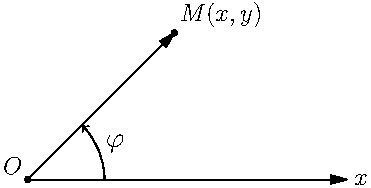
\includegraphics[width=6.5cm]{image/lecture-19.pdf}
    \end{center}
    $$\rho = |\overrightarrow{OM}|; \ \ \phi = \angle(Ox, \overrightarrow{OM})$$
    $$\begin{cases}
      x = \rho \cos(\phi)\\
      y = \rho \sin(\phi)
    \end{cases}$$ 
    $$z = \rho(\cos(\phi)+i\sin(\phi)); \ \ 
    \rho = |z| = \sqrt{x^2+y^2}$$
    $\bullet$ $\phi$ называется аргументом комплексного числа $z$, \ определяется с точностью до $2\pi k, \ k \in \Z$.
    $$Arg(z) = \phi + 2 \pi k, k \in \Z$$
    $$0\leq Arg(z)\leq2\pi - \text{главный аргумент}$$
    $$Arg(z) = \begin{cases}
      arctg(\frac{y}{x}), \tab[1.3cm] x>0 \\
      arctg(\frac{y}{x}+\pi), \tab[0.4cm] x<0
    \end{cases}$$ 
    Если $z = 0$, то аргумент не определяется (либо угол любой, либо $|z| = 0$)
    $$z_1 = z_2 \Longleftrightarrow \begin{cases}
      |z_1| = |z_2| \\
      \phi_1 = \phi_2 + 2\pi k, \ k\in \Z
    \end{cases}$$ 
  \end{definition} 
  \begin{subtheorem} (Формула Муавра)\\
    Пусть $z_1 = \rho_1(\cos(\phi_1) + i\sin(\phi_1)), \ \ z_2 = \rho_2(\cos(\phi_2) + i\sin(\phi_2))$ \\
    Тогда:
    \begin{enumerate}
      \item $z_1 \cdot z_2 = (\rho_1 \cdot \rho_2)(\cos(\phi_1+\phi_2) + i\sin(\phi_1+\phi_2))$
      \item если $z_2 \neq 0$, то $\frac{z_1}{z_2} = \frac{\rho_1}{\rho_2} (\cos(\phi_1-\phi_2) + i\sin(\phi_1-\phi_2))$  
    \end{enumerate}
  \end{subtheorem} 
  \begin{proof}\tab
    \begin{enumerate}
      \item
        $z_1 \cdot z_2 = \rho_1(\cos(\phi_1) + i\sin(\phi_1))\cdot \rho_2(\cos(\phi_2) + i\sin(\phi_2)) = \\ 
        \tab[4cm]=(\rho_1 \cdot \rho_2)(\cos(\phi_1)\cos(\phi_2) + i\sin(\phi_1)\sin(\phi_2)) = \\ 
        \tab[8cm]= (\rho_1 \cdot \rho_2)(\cos(\phi_1+\phi_2) + i\sin(\phi_1+\phi_2))$
      \item Аналогично
    \end{enumerate}
  \end{proof} 
  \begin{definition}
    Число $w \in \mathbb{C}$ называется корнем $n$-ой степени из $z\in \mathbb{C}$,\\ где $ n \in \N$, если $w^n = z$.
  \end{definition} 
  \begin{subtheorem}
    Пусть $z = \rho(\cos(\phi) + i\sin(\phi)), \ z \neq 0, \ n\in \N$\\
    Тогда $\exists$ ровно $n$ корней $n$-ой степени из $z\in \mathbb{C}$: \ $w_0, w_1,...,w_{n-1}$, причем: 
    $$w_l = \sqrt[n]{\rho}\cdot (\cos(\frac{\phi+2\pi l}{n})+i\sin(\frac{\phi+2\pi l}{n}))$$
    % \begin{center}
    %   \begin{tikzpicture}[scale=3]
    %     %\usetikzlibrary{calc}
    %     \draw[->] (-1.2,0) - - (1.5,0) node[right] {$Re(z)$};
    %     \draw[->] (0,-1.2) - - (0,1.5) node[left] {$Im(z)$};

    %     \coordinate (x0) at (0, 0);
    %     \coordinate (x1) at (1, 0);
    %     \coordinate (x2) at (0.8660254, 0.5);
    %     \coordinate (x3) at (0.5, 0.8660254);
    %     \coordinate (x4) at (0, 1);
    %     \coordinate (x5) at (-0.5, 0.8660254);
    %     \coordinate (x6) at (-0.8660254, 0.5);
    %     \coordinate (x7) at (-1, 0);
    %     \coordinate (x8) at (-0.8660254, -0.5);
    %     \coordinate (x9) at (-0.5, -0.8660254);
    %     \coordinate (x10) at (0, -1);
    %     \coordinate (x11) at (0.5, -0.8660254);
    %     \coordinate (x12) at (0.8660254, -0.5);

    %     \draw[fill] (x2) circle (0.8pt) node[above right] {$w_0$};
    %     \draw[fill] (x3) circle (0.8pt) node[above right] {$w_1$};
    %     \draw[fill] (x4) circle (0.8pt) node[above right] {$w_2$};
    %     \draw[fill] (x5) circle (0.8pt) node[above left] {$w_3$};
    %     \draw[fill] (x6) circle (0.8pt) node[above left] {$w_4$};
    %     \draw[fill] (x7) circle (0.8pt) node[above left] {$w_5$};
    %     \draw[fill] (x8) circle (0.8pt) node[below left] {$w_6$};
    %     \draw[fill] (x9) circle (0.8pt) node[below left] {$w_7$};
    %     \draw[fill] (x10) circle (0.8pt) node[below left] {$w_8$};
    %     \draw[fill] (x11) circle (0.8pt) node[below right] {$w_9$};
    %     \draw[fill] (x12) circle (0.8pt) node[below right] {$w_{10}$};
    %     \draw[fill] (x1) circle (0.8pt) node[below right] {$w_{11}$};
    %     \draw[fill] (x0) circle (1pt) node[below left] {$O$};
    %     \draw (x0) circle (28.5pt);

    %     % \tkzMarkAngle[mark=,arc=ll,size=10pt] (x2, x0, x3);
    %     % \tkzLabelAngle[pos=0.6] (x2, O, x3) {$\frac{\phi}{n}$};

    %     \draw[->] (0,0) - - node[above] {$\sqrt[n]{\rho}$}(0.842, 0.484);
    %     \draw[->] (0,0) - - (0.484, 0.842);

    %     \draw (1,0) - - (0.8660254, 0.5);
    %     \draw (0.8660254, 0.5) - - (0.5, 0.8660254);
    %     \draw (0.5, 0.8660254) - - (0,1);
    %     \draw (0,1) - - (-0.5, 0.8660254);
    %     \draw (-0.5, 0.8660254) - - (-0.8660254, 0.5);
    %     \draw (-0.8660254, 0.5) - - (-1,0);
    %     \draw (-1,0) - - (-0.8660254, -0.5);
    %     \draw (-0.8660254, -0.5) - - (-0.5, -0.8660254);
    %     \draw (-0.5, -0.8660254) - - (0, -1);
    %     \draw (0, -1) - - (0.5, -0.8660254);
    %     \draw (0.5, -0.8660254) - - (0.8660254, -0.5);
    %     \draw (0.8660254, -0.5) - - (1,0);

    %   \end{tikzpicture}
    % \end{center}

    \begin{center}
      % \begin{asy}
      %   unitsize(2.3cm);
      %   import graph;
      %   filldraw(Circle((0,0),1), white);
      %   pair O = (0,0);
      %   pair B = (1,0);
      %   dot("$O$", O, NW);
      %   draw((-1.25,0)--(1.35,0), Arrow);
      %   draw((0,-1.25)--(0,1.35), Arrow);
      %   label("$Re(z)$",(1.35, 0), SE); 
      %   label("$Im(z)$",(0, 1.35), NW);
      %   pair [] w;
      %   w[0] = (0.8660252, 0.5);
      %   w[1] = (0, 1);
      %   w[2] = (-0.8660252, 0.5);
      %   w[3] = (-0.8660252, -0.5);
      %   w[4] = (0, -1);
      %   w[5] = (0.8660252, -0.5);
      %   dot("$w_{1}$",w[1], NW);
      %   dot("$w_{2}$",w[2], NW);
      %   dot("$w_{3}$",w[3], SW);
      %   dot("$w_{4}$",w[4], SE);
      %   dot("$w_{5}$",w[5], SE);
      %   draw(w[0]--w[1]--w[2]--w[3]--w[4]--w[5]--cycle);
      %   draw((0, 0) -- w[0], Arrow);
      %   label("$\sqrt{\rho}$",(0.5, 0.27), NW);
      %   transform r1=rotate(60,O);
      %   dot("$w_0$",r1*w[5], NE); // интересно
      %   path p = scale(0.5)*(dir(B){up}..dir(r1*w[5]));
      %   draw(scale(1.15)*Label("$\frac{\varphi}{n}$"), p, Arrow(TeXHead));
      % \end{asy}
      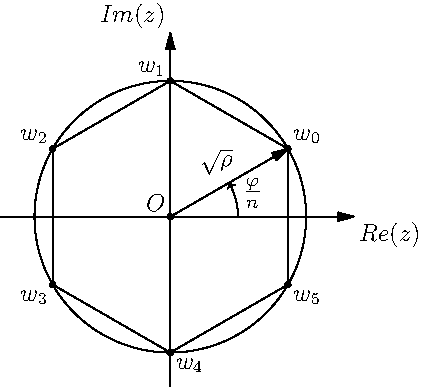
\includegraphics[width=6.5cm]{image/lecture-20.pdf}
    \end{center}
    $w_0, w_1,...,w_{n-1}$  - лежат в верщинах правильного $n$ - угольника, вписанного в окружность.  
  \end{subtheorem} 
  \begin{proof}
    Рассмотрим $w = r(\cos(\psi) + i\sin(\psi))$ 
    $$z = \rho(\cos(\phi) + i\sin(\phi)) = r^n(\cos(n\psi) + i\sin(n\psi)) = w^n$$
    $\Longrightarrow \begin{cases}
      r^n = \rho\\
      n \phi = \phi + 2 \pi k, k\in \Z
    \end{cases} \Longrightarrow w = \sqrt[n]{\rho}\cdot (\cos(\frac{\phi+2\pi k}{n})+i\sin(\frac{\phi+2\pi k}{n})), \ k \in \Z$\\ $\\$ 
    при $ k = \{0,1,...,k-1\}$ - $w$ принимает все различные значения.  
  \end{proof} 
  \begin{example1}
    $z=1,\ n=3, \ \sqrt[3]{1}$ 
  \end{example1}
  \begin{center}
    % \begin{asy}
    %   unitsize(2cm);
    %   import graph;
    %   filldraw(Circle((0,0),1), white);
    %   pair O = (0,0);
    %   dot("$O$", O, SW);
    %   draw((-1.25,0)--(1.4,0), Arrow);
    %   draw((0,-1.25)--(0,1.4), Arrow);
    %   label("$Re(z)$",(1.35, 0), SE); 
    %   label("$Im(z)$",(0, 1.35), NW);
    %   pair w0 = (1, 0);

    %   real a = 120;
    %   real b = -120;
    %   transform r1=rotate(a,O);
    %   transform r2=rotate(b,O);

    %   draw("$w_0$", w0, NE);
    %   draw("$w_1$",r1*w0,NW);
    %   draw("$w_2$",r2*w0,SW);

    %   draw(w0--r1*w0--r2*w0--cycle);

    %   draw(O--r1*w0, Arrow);

    %   // label("$\sqrt{\rho}$",(0.5, 0.27), NW);

    %   path p = scale(0.23)*(dir(w0){up}..dir(r1*w0));
    %   draw(scale(1.15)*Label("$\frac{2\pi}{3}$"), p, Arrow(TeXHead));
      
    % \end{asy}
    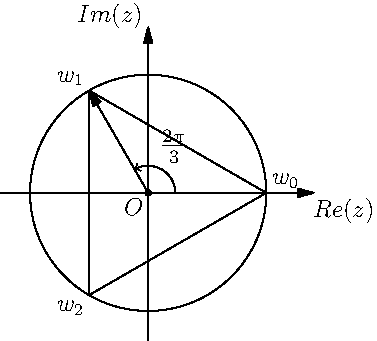
\includegraphics[width=6.5cm]{image/lecture-21.pdf}
  \end{center}
  \section{Алгебра над полем}
  Пусть $F$ - поле 
  \begin{definition}
    Алгеброй над полем $F$ называется множество $A$  с операциями сложения, умножения и умножения на элементы поля, удовлетворяет следующим аксиомам:
    \begin{enumerate}
      \item $(A, +, \cdot)$ - кольцо
      \item $(A, +, \lambda \cdot)$ - векторное пространство над полем $F$
      \item $\forall a, b \in A, \lambda\in F: \ \ \lambda(a \cdot b) = (\lambda a)b = a(\lambda b)$    
    \end{enumerate}
    Обозначается: $(A, +, \cdot, \lambda \cdot)$, \ \ $\lambda\in F$ 
  \end{definition}
  \begin{definition}
    Алгебра над полем называется коммутативной (ассоциативной, с единицей и т.д.), если алгебра, как кольцо, имеет соответствующее свойство.
  \end{definition}
  \begin{definition}
    Размерность алгебры - размерность алгебры, как векторного пространства над полем.
  \end{definition} 
  \begin{example}\tab
    \begin{enumerate}
      \item $M_n(F) -$ алгебра матриц с коэффициентами из $F$ (это НЕ коммутативная, ассоциативная с единицей алгебра над $F$)
      \item $(V^3, +, \times, \lambda \cdot)$ - векторное произведение (НЕ коммутативна, НЕ ассоциативная без единицы алгебра над $\R$, размерности 3)
      \item $L$ - подполе поля $F \Longrightarrow F$ можно рассматривать, как алгебру над $L$  
      \begin{example1}
        $\mathbb{C}$ - алгебра над $\R$ размерности 2 (Базис: $\{1, i\}$) 
      \end{example1}
    \end{enumerate}
  \end{example}
  Пусть $A$ - алгебра над полем $F$, \ $\{e_1,...,e_n\}$ - базис алгебры $A$, как векторного пространства, тогда $$\forall a, b \in A: a = \sum \limits_{j=1}^na_je_j, \ b = \sum \limits_{j=1}^na_je_j$$ 
  $$\Longrightarrow a \cdot b = (\sum \limits_{j=1}^na_je_j)(\sum \limits_{j=1}^na_je_j) = \sum \limits_{j,k=1}^na_jb_k(e_je_k)$$ 
  Для умножения произвольных элементов достаточно знать таблицу умножения базисных элементов $(e_j \cdot e_k)$ 
  \begin{subtheorem}
    Для проверки коммутативности $(\cdot)$ в алгебре (ассоциативности и т.д.) достаточно проверить на базисных векторах. 
  \end{subtheorem} 
  \begin{proof}
    Очевидно
  \end{proof}
  \begin{example}\tab
    \begin{enumerate}
      \item $\mathbb{C}$ - алгебра над $\R$ с базисом $\{1, i\}$
      $$\begin{tabular}{c|cc}
        \null & 1 & i \\ \hline
        1 & 1 & i \\
        i & i & -1
      \end{tabular}$$
      \item $(V^3, +, \times, \lambda \cdot); \  \ V^3$ c базисом $\{i, j, k\}$
      $$\begin{tabular}{c|c|c|c}
        x & i & j & k \\ \hline
        i & 0 & k & j \\ \hline
        j & -k & 0 & i \\ \hline
        k & -j & -i & 0
      \end{tabular}$$
      \item $M_n(F)$
    \end{enumerate}
  \end{example}
  \begin{remark}
    Пусть $V$ - векторное пространство над полем $F$.
  Хотим превратить $V$ в алгебру над полем $F$. \\
  Пусть $e_{jk}$ - произвольные векторы из $V, \ j,i = \overline{1, n}$ \\
  Положим $e_j \cdot e_k = e_{jk} \Longrightarrow $ $$\forall a, b\in V: \ a\cdot b=\sum \limits_{j,k=1}^na_jb_ke_{jk}$$
  Это произведение превращает $V$ в алгебру над полем $F$.  
  \end{remark} 
  \begin{example1}
    Алгебра кватернионов $\mathbb{H}$ \\
    $\mathbb{H}$ - 4-х - мерное векторное пространство над $\R$ с базисом $\{1, i, j, k\}$ и таблицей умножения:
    $$\begin{tabular}{c|c|c|c|c}
        \null & 1 & i & j & k \\ \hline
        1 & 1 & i & j & k \\ \hline
        i & i & -1 & k & -j \\ \hline
        j & j & -k & -1 & i \\ \hline
        k & k & j & i & -1
      \end{tabular}$$
      $\Longrightarrow $ ассоциативная, НЕ коммутативная алгебра, в которой каждый не нулевой элемент обратим (тело).  
  \end{example1}
  \begin{definition}
    Подмножество $B$ алгебры $A$ назвается подалгеброй $A$, если $B$ - подпространство $A$, как кольца, и подпространства $A$, как пространства.      
  \end{definition} 
  \begin{subtheorem}
    Любоя подалгебра сама является алгеброй относильно тех же оперций и тем же полем.
  \end{subtheorem} 
  \begin{definition}
    Алгебра $A$ и $\widetilde{A}$ над одним и тем же полем назваются изоморфными, если они изоморфны. 
  \end{definition}

  \subsection{Алгебра многочленов над полем}
  $F$ - поле
  \begin{definition}
    Бесконечная последовательность $(a_0,a_1, a_2,...)$, где $a_i \in \R$, называется финитной, если только конечное число $a_i$ отлично от нуля. 
    $$F^{\infty} = \{(a_0,a_1, a_2,...) \ |\ a_i \in \R\}$$ 
  \end{definition}  
  \begin{subtheorem}
    Множество $F^{\infty}$ относительно операции сложения: $$(a_0,a_1, a_2,...) + (b_0,b_1, b_2,...) = (a_0+b_0,a_1+b_1, a_2+b_2,...)$$ и умножения на элементы $\lambda \in F$: $$(a_0,a_1, a_2,...) \cdot \lambda = (\lambda a_0,\lambda a_1, \lambda a_2,...)$$
    $F^{\infty}$ - бесконечномерное векторное пространство.   
  \end{subtheorem} 
  \begin{subtheorem}
    $F^{\infty}$ - счетномерно с базисом:
    $$(e_0,e_1,e_2,...) = ( \ (1, 0, 0, ...), \ (0, 1, 0, ...), \ (0, 0, 1, ...), ... \ )$$ 
    Зададим умножение $e_k \cdot e_l = e_{k+l} \Longrightarrow F^{\infty}$  превращается в алгебру над полем $F$ 
  \end{subtheorem} 
  \begin{remark}
    Так как $e_l = e_{k+l}$ и в $\Z$ сложение коммутативно и ассоциативно, то $F^{\infty}$ - ассоциативная, коммутативная алгебра над $F$ с единицей: $e_0 = (1, 0, 0, ...)$
  \end{remark} 
  \begin{definition}
    Такая алгебра называется алгеброй многочленов над полем $F$. 
    Обозначается: $F[x]$  
  \end{definition} 
  Получаем привычный вид многочлена: 
  $\forall a \in F: \ a\cdot e_0$ отожествим с элементом $a$, а вектор $e_1$ обозначим через $x$:
  $$e_k = \underbrace{e_1 \cdot e_1 \cdot ... \cdot e_1}_{k}  = x^k$$     
  Рассмотрим произвольный $(a_0,a_1, a_2,...) \in F^{\infty}$. Так как она финитная, то: 
  $$(a_0,a_1, ..., a_n,0, 0,...) = a_0e_0 + a_1e_1+...+a_ne_n = a_0 + a_1x+...+a_nx^n$$
  $a_i$ называется коэффициентом многочлена.
  \begin{definition}
    Если $f = a_0 + a_1x+...+a_nx^n$, где $a_n \neq 0$, $a_k = 0,  \ \forall k>n$, то $a_n$ называется старшим членом, а число $\deg f = n$  называется степенью многочлена.  
  \end{definition} 
  \begin{remark}
    $\deg 0 = -\infty$ (или неопределена)\\
    $f\neq 0, \ \deg f \in \N \cup \{0\}$  
  \end{remark} 
  \begin{properties}\tab
    \begin{enumerate}
      \item $\deg (f+g) \leq \max \{\deg f, \deg g\}$
      \item $\deg (fg) = \deg f + \deg g$  
    \end{enumerate}
  \end{properties}
  \begin{proof} \tab
    \begin{enumerate}
      \item Упражнение
      \item $$f = a_0 + a_1x+...+a_nx^n, \ a_n, \ \deg f = n$$
      $$g = b_0 + b_1x+...+b_mx^m, \ b_m, \ \deg f = m$$
      $$fg = a_0b_0 +...+a_nb_mx^{n+m}$$
      $a_n, b_m \neq 0$, т.к. в поле нет делителей нуля 
      $\Longrightarrow a_nb_m$ - старший член $$\Longrightarrow \deg fg = \deg f + \deg g$$     
    \end{enumerate}
  \end{proof}
  \begin{consequense}\tab
    \begin{enumerate}
      \item в $F[x]$ нет делителей нуля.
      \item Обратные в $F[x]$ - это многочлены нулевой степени и только они, т.е. это все ненулевые константы. 
    \end{enumerate}
  \end{consequense} 
  \subsubsection{Деление с остатком}
  \begin{theorem}
    Пусть $F$ - поле, \ $f, g \in F,\ g\neq 0 $. Тогда $\exists ! \ q, r$: \ $f = g \cdot q + r$, \\причем либо $r=0$, либо $\deg r < \deg g$       
  \end{theorem}
  \begin{proof}
    Пусть $f, g \neq 0$$$f = a_0 + a_1x+...+a_nx^n, \ a_n \neq 0, \ \deg f = n$$ $$g = b_0 + b_1x+...+b_mx^m, \ b_m \neq 0, \ \deg f = m$$ 
    \textit{Докажем существование:} 
    \begin{enumerate}
      \item $n<m \Longrightarrow f = 0 \cdot g + f \ (q=0, f = r)$
      \item $n\geq m \Longrightarrow f_1 = f - \frac{a_n}{b_m} \cdot g \cdot x^{n-m}$ \\
      Если $\deg f_1 < \deg g \Longrightarrow r = f_1, \ q = \frac{a_n}{b_m}\cdot x^{n-m}$ \\
      Иначе продолжаем процесс с $f_1$ (заметим, что $\deg f_1 < \deg f$): находим $f_2 $ и т.д. Процесс закончится на конечном шаге.  
    \end{enumerate}
    \textit{Докажем единственность:}  \\
    Допустим, $ f = g \cdot q_1 + r_1$ и $f = g \cdot q_2 + r_2$ $$  \Longrightarrow r_1 - r_2 = g(q_2 - q_1) \Longrightarrow \deg (r_1-r_2) = \deg g + \deg (q_2 - q_1) $$ $$\deg(r_1 - r_2) \geq \deg g$$. С другой стороны $$\deg (r_1-r_2) < \max \{\deg r_1, \deg r_2\} < \deg g$$ - получаем противоречие.   
  \end{proof} 
  \subsubsection{Мгогочлены как функции}
  $F$ - поле, \ $f = a_nx^n + a_{n-1}x^{n-1} +...+ a_0$
  \begin{definition}
    Значение многочлена $f$ в точке $c$ называет число, равное: $$a_nc^n + a_{n-1}c^{n-1} +...+ a_0$$
     Таким образом, множество $f$ задает отображение $F \to F$
     $$c \to f(c) \Longrightarrow f \text{ задает функцию}$$      
  \end{definition} 
  \begin{remark}
    Разные многочлены могут задавать одну функцию.
  \end{remark} 
  \begin{example1}
    $F = \Z_2, \ f_1 = x^2, \ f_2 = x$ - разные многочлены, но они задают одну и ту же функцию:
    $$f_1(0)=0, \ f_1(1) = 1, \ f_2(0)=0, \ f_2(1) = 1$$ 
  \end{example1}
  \begin{theorem}
    Пусть $F$ - бесконечное полею. Тогда разные многочлены задают разные функции. 
  \end{theorem} 
  \begin{proof}
    Допустим, $f, g \in F[x], \ f \neq g, \ \forall c \in F, \ f(c) = g(c)$ \\
    Введем $h = f - g \in F[x], \ h \neq 0, \ \forall c \in F, \  h(c)=0$\\
    Т.к. поле $F$ - бесконечное, то $\exists \ c_0, c_1,...,c_n \in F$ - различные числа, такие что:
    $$\begin{cases}
      h(c_0) = 0 \\
      h(c_1) = 0 \\
      \vdots \\
      h(c_n) = 0 
    \end{cases} \Longrightarrow \ \ 
    \begin{cases}
      a_nc_0^n + a_{n-1}c_0^{n-1} + ... + a_1c_0+ a_0 = 0 \\
      a_nc_1^n + a_{n-1}c_1^{n-1} + ... + a_1c_1+ a_0 = 0 \\
      \vdots \\
      a_nc_n^n + a_{n-1}c_n^{n-1} + ... + a_1c_n+ a_0 = 0
    \end{cases}$$ - квадратная однородная СЛУ относительно неизвестных $a_n, a_{n-1}, ..., a_0$ с матрицей коэффициентов $A:$
    $$A = \begin{pmatrix}
      c_0^n & \cdots & c_0^1 \\
      c_1^n & \cdots & c_1^1 \\
      \vdots & \null & \vdots\\ 
      c_n^n & \cdots & c_n^1 \\
    \end{pmatrix}, \ \ \det A = (-1)^2 \cdot \underbrace{V(c_0, c_1,...,c_n)}_{\text{Определитель Вандермонда}}$$
    $\Longrightarrow $ по правилу Крамера СЛУ имеет единственное решение и оно тривиальное $\Longrightarrow  \forall i \in \{0, 1,...,n\}: a_i = 0 \Longrightarrow n=0$ противоречие.    
  \end{proof}
  
  \begin{theorem}\textbf{(Безу)} 
    Пусть $F$ - поле, $ \ f \in F[x], c \in F$.\\
    Тогда остаток при делении $f$ на $(x-c)$ равен значению многочлена в точке $c$.     
  \end{theorem}
  \begin{proof}
    Пусть $f(x) = (x-c)g(x) + r(x)\  (*)$
    $$\deg r(x) < \deg (x-c) = 1 \Longrightarrow  r(x) - const$$
    $\Longrightarrow $ Либо $r(x) = 0$, либо $r(x)=r \in F$\\
    Подставим в $(*) \ x = c$:
    $$f(c) = (c-c)\cdot q(c) + r(c) = r$$
  \end{proof}   
  \subsubsection{Корни многочленов}
  \begin{definition}
    Элемент $c\in F$ - корень многочлена $f \in F[x]$, если $f(c) = 0$. Из теоремы Безу получаем утверждение: 
  \end{definition}
  \begin{subtheorem}
    $c \in F$ - корень многочлена $f\in F[x] \Longleftrightarrow (x-c) \ | \ f$.  
  \end{subtheorem}  
  \begin{definition}
    Если $c$ - корено многочлена $f$ и $(x-c)^2 \nmid f$, то корень $c$ - называется простым, иначе - кратным.
  \end{definition} 
  \begin{definition}
    Если $c$ - корень и $(x-c)^k \ | \ f, (x-c)^{k+1} \nmid f$, то $c$ - корень кратности $k$ \ $(k \in \N)$.     
  \end{definition} 
  \begin{subtheorem}
    $c$- корень многочлена $f$ кратности $k \Longleftrightarrow \begin{cases}
      f = (x-c)^k \cdot g\\
      g(c) \neq 0
    \end{cases}$  
  \end{subtheorem} 
  \begin{consequense}
    Пусть $f \in F[x], \ f \neq 0, \ \deg f = n, \ k$ - число всех корней многочлена $f$ с учетом кратности. \\
    Тогда $k\leq n$, причем если $k=n \Longleftrightarrow f$ раскладывается на линейные многочлены.    
  \end{consequense}
  \begin{proof}
    Если $c_1$ - корень, то $f = (x-c_1)g_1$ \\
    \tab[4.1cm]Если $c_2$ - корень, то $f = (x-c_1)(x-c_2)g_2$ и т.д. 
    $$\Longrightarrow f = (x-c_1)(x-c_2)...(x-c_k)g$$
    где $g$ не имеет корней. То есть $c_1,...,c_k$ - корни многочлена $f$, при этом среди них могут быть одинаковые.
    $$\Longrightarrow f = (x-\widetilde{c_1})^{k_1}(x-\widetilde{c_2})^{k_2}...(x-\widetilde{c_s})^{k_s}g$$
    где $\widetilde{c_1},...,\widetilde{c_s}$ - все различные корни.\\ Т.к. $$f = (x-\widetilde{c_l})h$$ 
    где $h(\widetilde{c_l}) \neq 0 \Longrightarrow \widetilde{c_l}$ - корень кратности $k_l$ $$\Longrightarrow \deg f = k_1 +...,+k_s + \deg g \Longrightarrow k = k_1+...+k_s \leq n$$
    При этом: $$k=n \Longleftrightarrow \deg g =0 \Longleftrightarrow f = \prod\limits_{l=1}^{s}(x-\widetilde{c_l})^{k_l}$$       
  \end{proof}
  \begin{definition}
    Формальной производной многочлена 
    $$f = a_nx^n + a_{n-1}x^{n-1} + ... + a_0$$
    называется многочлен:
    $$f' = a_nnx^n + a_{n-1}(n-1)x^{n-1} + ... + a_1$$  
  \end{definition}
  \begin{subtheorem}\tab
    \begin{enumerate}
      \item $(f+g)' = f'+g'$
      \item $(\alpha f)' = \alpha f'$
      \item $(fg)' = f'g+fg'$   
    \end{enumerate}
  \end{subtheorem}
  \begin{subtheorem}
    Пусть $\textrm{char} F = 0, \ c \in F, \ f \in F[x]$, \ тогда: 
    $$f(x)=f(c) + \frac{f'(c)}{1!}(x-c) + \frac{f^{(2)}(c)}{2!}(x-c)^2 + ... + \frac{f^{(n)}(c)}{n!}(x-c)^n$$ 
  \end{subtheorem}
  \begin{proof}
    $f(x) = a_nx^n + a_{n-1}x^{n-1} + ... + a_0$.\\ Подставим $x = y+c$: 
    $$f = b_ny^n + b_{n-1}y^{n-1} + ... + b_0$$
    Подставим $y = x - c$:
    $$f = b_n(x-c)^n + b_{n-1}(x-c)^{n-1} + ... + b_0$$ 
    $\Longrightarrow f^{(k)}(c) = k! \cdot b_k$ (вопросик)
  \end{proof}
  \begin{consequense}
    Пусть $\textrm{char} F = 0, \ f \in F[x], c\in F$\\
    Тогда $c$ - корень многочлена $f$ кратности $k \Longleftrightarrow \begin{cases}
      f(c) = 0\\
      f'(c) = 0\\
      \vdots \\
      f^{(k-1)}(c) = 0\\
      f^{(k)}(c) \neq 0
    \end{cases}$    
  \end{consequense}    
  \subsection{Основная теорема алгебры}
  \begin{theorem}
    Любой многочлен над полем комплексных числел положительной степени имеет хотя бы один корень.
  \end{theorem}
  \begin{subtheorem}\tab
    \begin{properties}\tab
      $\forall z_1, z_2 \in \mathbb{C}$
      \begin{enumerate} 
        \item $|z_1+z_2|\leq |z_1| + |z_2|$
        \item $||z_1|-|z_2||\leq |z_1-z_2|$ 
      \end{enumerate}
      \begin{proof}
        Из свойств векторов \ ($z = x+iy$ - вектор, $\sqrt{x^2+y^2}$ - длина вектора)
      \end{proof} 
    \end{properties}
  \end{subtheorem}
  \begin{definition}
    Последовательность $\{z_k\}_{k=1}^{\infty} \subseteq \mathbb{C}$ называется сходящейся к $z_0 \in \mathbb{C}$ , если $|z_k-z_0| \to 0, \ k\to \infty$\\
    Обозначается: $z_k \to z_0, \ k\to \infty$ 
  \end{definition} 
  \setcounter{lemcount}{0}
  \begin{lemmanum}
    Пусть $z_k = x_k+iy_k, \ z_0 = x_0 + iy_0$, тогда:
    $$z_k \to z_0 \Longleftrightarrow \begin{cases}
      x_k \to x_0 \\
      y_k \to y_0
    \end{cases}$$  
  \end{lemmanum} 
  \begin{proof}
    Следует из равенства $|z_k-z_0| = \sqrt{x^2+y^2}$ 
  \end{proof} 
  \begin{lemmanum}
    Если $z_k \to z_0$, то $|z_k| \to |z_0|$  
  \end{lemmanum} 
  \begin{proof}
    Т.к. $||z_k|-|z_0||\leq |z_k-z_0|$ 
  \end{proof} 
  \begin{lemmanum}
    Если $z_k \to z_0, \ w_k \to w_0$, то:
    \begin{enumerate}
      \item $z_k + w_k \to z_0 + w_0$
      \item $z_k \cdot w_k \to z_0 \cdot w_o$  
    \end{enumerate}
  \end{lemmanum} 
  \begin{proof}
    Упражнение.
  \end{proof} 
  \begin{consequense}
    Если $f \in \mathbb{C}[z], \ \deg f >0, \ z_0 \in \mathbb{C}, \ z_k \to z_0$, тогда: 
    $$f(z_k) \to f(z_0)$$  
  \end{consequense}
  \begin{lemmanum} \textbf{О возрастании модуля} $|f(z)|$ \\
    Пусть $f \in \mathbb{C}[z], \ \deg f >0$, тогда если $|z_k| \to \infty$, то:
    $$|f(z_k)| \to \infty$$        
  \end{lemmanum} 
  \begin{proof}
    $f(z) = a_nx^n + ... + a_1x+a_0 \in \mathbb{C}[z] \neq 0$
    \begin{multline*}
      |f(z_k)| = a_nz_k^n + a_{n-1}z_k^{n-1}... + a_1z_k+a_0 \geq \\
      \geq |z_k|^n \cdot ||a_n|-\frac{|a_{n-1|}}{|z_k|} - ... - \frac{|a_{1|}}{|z_k|^{n-1}} - \frac{|a_{0|}}{|z_k|^{n}}| \to \infty
    \end{multline*} 
  \end{proof} 
  \begin{lemmanum}\textbf{(Лемма Даламбера)} \\
    Пусть $f \in \mathbb{C}[z], \ \deg f >0, \ f(z_0) \neq 0$, тогда $\exists$ $z \in \mathbb{C}$ сколько угодно близкое  к $z_0$ такое, что:
    $$|f(z)|< |f(z_0)|$$ 
  \end{lemmanum} 
  \begin{proof}
    Разложим $f$ по степеням $(z-z_0)$:
    $$f(z) = f(z_0) + b_s(z-z_0)^s + ... + b_n(z-z_0), \ \text{ где } b_s \neq 0$$
    Так как $f(z_0) \neq 0$, то можно поделить на него:
    $$\frac{f(z)}{f(z_0)} = 1 + c_s(z-z_0)^s + ... + c_n(z-z_0), \ c_i = \frac{b_i}{f(z_0)} \neq 0$$  
    Найдем $z_1 \in \mathbb{C}: \ c_sz_1^s = -1$
    \begin{center}
      % \begin{asy}
      %   unitsize(2cm);
      %   dot("$O$", (0,0), NW);
      %   dot("$z_0$", (0.4, 0.33));
      %   dot("$z ?$", (0.8, 0.66));
      %   dot("$z_1+z_0$", (1.22, 1.00));
      %   draw((0.4, 0.33) -- (1.2, 0.99), Arrow(TeXHead));
      %   draw((-0.25,0)--(2,0), Arrow);
      %   draw((0,-0.25)--(0,1.6), Arrow);
      %   label("$Re(z)$",(1.9, 0), SE); 
      %   label("$Im(z)$",(0, 1.5), NW);
      % \end{asy}
      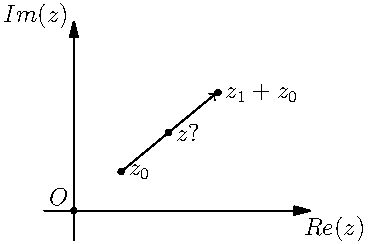
\includegraphics[width=6.5cm]{image/lecture-22.pdf}
    \end{center}

    \begin{center}
      Рассмотрим $z = z_0 + tz$, где $t \in (0,1)$
    \end{center}
    Подставим: 
    $$\frac{f(z)}{f(z_0)} = 1 - t^s + t^{s+1} g(t), \text{ где } g(t) \in \mathbb{C}, \ \deg g \leq n-(s-1)$$
    $$|g(t)| = |\alpha_0 + \alpha_1t + ... + \alpha_{n-(s+1)}t^{n-(s+1)}|$$ 
    Обозначим $C = \max\{|\alpha_i|\}$, тогда $|g(t)|\leq C(n-s)$
    \begin{multline*}
      |\frac{f(z)}{f(z_0)}| = |1 - t^s + t^{s+1} g(t)| \leq |1 - t^s| + t^{s+1} |g(t)| \leq \\ \leq 1 - t^s + t^{s+1} C(n-s) = 1 - t^s(1-+ tC(n-s)) \underbrace{<}_{\text{хотим}} 1
    \end{multline*} 
     $$1-tC(n-c)>0 \Longleftrightarrow \frac{1}{C(n-s)}$$
     Выбираем такое $t \in (0,1)$ и получаем:
     $$1-t^s(1-tC(n-s)) < 1$$
     Если $C=0$, то верно и очевидно.   
  \end{proof}
  \begin{theorem} \textbf{(Основная теорема алгебры)} 
    $$\forall f \in \mathbb{C}[z], \ \deg f >0 \Longrightarrow  \exists \ z_0 \in \mathbb{C}: \ f(z_0) = 0$$
  \end{theorem}
  \begin{proof}
    Рассмотрим $M = \underbrace{\inf}_{z} |f(z)|$
    \begin{itemize}
      \item[\textit{1 шаг.}] Хотим доказать, что $\inf$ достигается, т.е. $\exists \ z_0 \in \mathbb{C}: \ |f(z_0)| = M$\\
      По определению $\inf \exists$ последовательность $\{z_k\}: \ |f(z_k)| \to M$
      \begin{itemize}
        \item[1 случай.] $\{z_k\}$  - не ограничена, т.е. $\exists \subseteq \{z_{i_k}\}: \ |z_{i_k}| \to \infty$. \\
        По лемме (4): \ $|f(z_{k_i})| \to \infty$ - противоречие. 
        \item[2 случай.] $\{z_k\}$ - ограничена $\Longrightarrow \exists \ C > 0: \ |z_k | < C \Longrightarrow$   
        $$\begin{matrix}
          |x_k|<|z_k|<C \\
          |y_k|<|z_k|<C
        \end{matrix} \ \ \ \text{ где } z_k = x_k + iy_k$$
        Так как $\{x_n\}, \{y_k\}$ - ограничены, то по теореме Больцано-Вейштрасса:
        $$\exists \ \{x_{k_{i}}\}\subseteq \{x_{k}\}: \ \{x_{k_{i}}\} \to x_0$$
        $$\exists \ \{y_{k_{i_l}}\}\subseteq \{y_{k_{i}}\}: \ \{y_{k_{i_l}}\} \to y_0$$
        Значит по Лемме (1):
        $$\{z_{k_{i_l}}\} \to x_0 + iy_0 = z_0 \Longrightarrow |f(\{z_{k_{i_l}}\})| \to |f(z_0)| = M$$  
      \end{itemize}
      \item[\textit{2 шаг.}] Допустим, что $M>0 \Longrightarrow$ по Лемме (5):
      $$\exists \ \widetilde{z} \in \mathbb{C}: \ |f(\widetilde{z})|<M = f(z_0) - \text{противоречие, т.к. } M - \inf $$
      $$\Longrightarrow M=0 \Longrightarrow f(z_0) =0$$  
    \end{itemize}
  \end{proof} 
  \begin{consequensenum}
    Любой многочлен над $\mathbb{C}$ положительной степени раскладывается на линейные множители. 
  \end{consequensenum}
  \begin{consequensenum}
    Любой многочлен над $\mathbb{C}$ степени $n$ имеет $n$ корней с учетом кратности. 
  \end{consequensenum} 
  \begin{example1}
    Пока что впадлу
  \end{example1}
  \begin{theorem}\textbf{(О мнимых корнях многочлена с вещественными коэффициентами)} \\
    Пусть $f \in \R[x], \ c$ - корень, \ $c \in \mathbb{C}\setminus \R$ и пусть этот корень имеет кратность $k$, тогда $\overline{c}$ - тоже корень многочлена $f$ кратности $k$.     
  \end{theorem} 
  \begin{proof}
    $f(x) = a_nx^n+...+a_1x+a_0, \ a_i \in \R$, \ $c$ - корень $\Longrightarrow f(c) =0$  
    $$f(\overline{c}) = a_n\overline{c}^n+...+a_1\overline{c}+a_0 = a_nc^n+...+a_1c+a_0 = f(c) = 0$$  ХЗ \\
    Кратность одинаковая, т.к. $f^{(s)}(c)=0 \Longleftrightarrow f^{(s)}( \overline{c})=0$ 
  \end{proof}
  \begin{theorem}
    Любой многочлен над $\R$ положительной степени раскладывается на линейные множители и квадратные множители с отрицательным дискриминантом.
  \end{theorem}
  \begin{proof}
    $f\in \R[x] \subseteq \mathbb{C}[x] \Longrightarrow $ (по следствию 1 и ОТА) \\
    $\alpha_1,...,\alpha_s \in \R$ - все корни кратности $k_1,..,k_s$\\
    $c_1,...,c_t \in \mathbb{C}\setminus \R$ - мнимые корни кратности $m_1,...,m_t$\\
    $\overline{c_1},...,\overline{c_t}$ - тоже мнимые корни, той же кратности $(c_1 \to \overline{c_1})$\\
    $\Longrightarrow \alpha_1,..,\alpha_s,c_1,...,c_t,\overline{c_1},...,\overline{c_t}$ - все корни многочлена
    $$f(x) = a_n \prod\limits_{j=1}^{s}(x-\alpha_j)^{k_j} \cdot \prod\limits_{\nu=1}^{t}(x-c_{\nu})(x-\overline{c_{\nu}})^{m_\nu} = (*)$$
    Если $c=a+bi \in \mathbb{C}\setminus \R$, то:
    $$(x-c)(x-\overline{c}) = x^2 - (c-\overline{c})x + c \overline{c}$$
    $$c+\overline{c} = 2a, \ \ c \overline{c} = a^2 + b^2$$
    $\Longrightarrow $ уравнение с отрицательным дискриминантом    
    $$(*) = a_n \prod\limits_{j}(x-\alpha_j)^k_j \cdot \prod\limits_{\nu}(\underbrace{x^2+\beta_{\nu}+ \gamma_{\nu}}_{D<0})^{m_\nu} $$    
  \end{proof}
  \begin{example1}
    $x^4 +1=0, \ x^4 = -1, \ w_k = \cos(\frac{\pi+2\pi k}{4})+ i\sin (\frac{\pi+2\pi k}{4})$
    \begin{multline*}
      \tab[2cm]x^4 +1= (x-w_0)(x-\overline{w_0})(x-w_1)(x-\overline{w_1}) = \\
      = (x^2 - \sqrt{2}x + 1)(x^2 + \sqrt{2}x + 1)\tab[1cm]
      \
    \end{multline*}
    \begin{center}
      % \begin{asy}
      %   unitsize(2cm);
      %   import graph;
      %   filldraw(Circle((0,0),1), white);
      %   dot((0,0));
      %   label(" $O$ ", (0.2, 0.09));
      %   draw((-1.25,0)--(1.35,0), Arrow);
      %   draw((0,-1.25)--(0,1.35), Arrow);
      %   label("$Re(z)$",(1.35, 0), SE); 
      %   label("$Im(z)$",(0, 1.35), NW);
      %   pair [] w;
      %   w[0] = (0.7071067, 0.7071067);
      %   w[1] = (-0.7071067, 0.7071067);
      %   w[2] = (-0.7071067, -0.7071067);
      %   w[3] = (0.7071067, -0.7071067);
      %   dot("$w_{0}$",w[0], NE); 
      %   dot("$w_{1}$",w[1], NW);
      %   dot("$w_{2}$",w[2], SW);
      %   dot("$w_{3}$",w[3], SE);
    
      %   draw((0, 0) -- w[0]);
      %   draw((0, 0) -- w[1]);
      %   draw((0, 0) -- w[2]);
      %   draw((0, 0) -- w[3]);
      % \end{asy}
      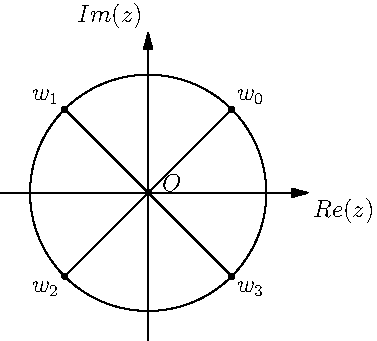
\includegraphics[width=6.5cm]{image/lecture-23.pdf}
    \end{center}
  \end{example1}

  \subsection{Неприводимые многочлены}
  $F$ - поле
  \begin{definition}
    Многочлен $f \in F[x], \ \deg f > 0$ называется неприводимым над полем $F$, если $f$ нельзя разложить в произведение многочленов $gh$, \\где $gh \in F[x], \ \deg g < \deg f, \ \deg h < \deg f$.
  \end{definition}
  \begin{subtheorem}
    Любой многочлен 1-ой степени является неприводимым над $F$. 
  \end{subtheorem}
  \begin{example1} 
    $x^2 + 1 \in \mathbb{C}[x]$ - приводимый
    $$x^2 + 1 = (x+i)(x-i)$$
    \tab[11cm]$x^2 + 1 \in \R[x]$ - неприводимый  
  \end{example1} 
  \begin{subtheorem}\textbf{(1)}
    Неприводимые многочлены над $\mathbb{C}$ - это линейные многочлены и только они. 
  \end{subtheorem}
  \begin{subtheorem}\textbf{(2)}
    Неприводимые многочлены над $\R$ - это все линейные многочлены и все квадратные многочлены с отрицательным дискриминантом и только такие.  
  \end{subtheorem}
  \begin{remark}
    Над любым полем $\exists$ бесконечное число непропорциональных\\ неприводимых многочленов.
  \end{remark}   
  \subsection{Многочлены от нескольких переменных}
  $F$ - поле, \ $n \in \N$ - фиксированная. \\
  Рассмотрим бесконечномерную алгебру над полем $F$ с базисом \\ $\{e_{k_1},...,e_{k_n} \ | \ k_i \in \N \cup \{0\} \} $ и умножением:
  $$e_{k_1},...,e_{k_n} \cdot \ e_{m_1},...,e_{m_n} = e_{k_1 + m_1},...,e_{k_n + m_n} \ (*)$$
  Эта алгебра называется алгеброй множеств от $n$ переменных над полем $F$. \\
  Обозначается: $F[x_1,...,x_n]$\\
  Из правила $(*)$ $\Longrightarrow $ , что алгебра коммутативна, ассоциативна, с единицей: $e_{0,...,0}$\\
  Отождествляем: \ $\alpha \in F \longleftrightarrow \alpha \cdot e_{0,...,0}$
  $$\begin{cases}
    e_{1,0,...,0} = x_1\\
    e_{0,1,...,0} = x_2\\
    \vdots\\
    e_{0,0,...,1} = x_n
  \end{cases} \Longrightarrow (\text{из } *) \ \ e_{k_1,...,k_n} = x_1^{k_1} \cdot ... \cdot x_n^{k_n} \Longrightarrow $$ 
  $\Longrightarrow $ произвольный элемент из алгебры (по определению базиса) раскладывается, как $$f = \sum \alpha_{k_1,...,k_n} \cdot e_{k_1,...,k_n} = \sum \alpha_{k_1,...,k_n} \cdot x_1^{k_1} \cdot ... \cdot x_n^{k_n}$$
  $$ f:= f(x_1,...,x_n)$$ 
  - многочлен над полем $F$.
  \begin{example1}
    $$f = x_1^5 x_2^7 x_3 - 5x_2^4x_3x_4 + 6x_2x_3 + 7$$
    Любой многочлен $f \in F[x_1,...,x_n]$ можно предствить в виде:
    $$(**) \ f = \sum \limits_{k=0}^sf_k(x_2,...,x_n)x_1^k \Longrightarrow $$
    $\Longrightarrow$ кольцо $F[x_1,...,x_n]$ можно рассматривать, как кольцо многочленов от $x_1$ с коэффициентами из кольца $F[x_2,...,X_n]$.\\
    Как и для $n=1$, многочлен $f \in F[x_1,...,x_n]$ задает функцию из $F^n = F \times ... \times F$.      
  \end{example1} 
  \begin{theorem}
    Если поле $F$ - бесконечно, то разные многочлены из $F[x_1,...,x_n]$ задает разные функции.
  \end{theorem}
  \begin{proof}
    Идея: индукция по $n$. База: $n=1$ - было доказано.\\
    $n-1 \to n$. Рассмотром разложение многочленов в виде $(**)$\\
    Доказательство д/з (   
  \end{proof}
  \subsection{Лексикографический порядок на одночленах}
  $\alpha x_1^{k_1} \cdot ... \cdot x_n^{k_n}$ - одночлен, $\alpha \in F$.
  \begin{definition}
    Порядок $\alpha x_1^{k_1} \cdot ... \cdot x_n^{k_n}\succ \beta x_1^{k_1} \cdot ... \cdot x_n^{k_n}$ \ $(\alpha, \beta \neq 0)$, называется лексикографическим, если:
    $$\exists \ s =\overline{0,n-1}: k_1=m_1 \ ,...,\ k_s=m_s, \ k_{s+1} > m_{s+1}$$
  \end{definition}
  \begin{example1}
    $$3x_1^{30}x_2^7 \succ 5x_1^{10}x_2^{150}$$
  \end{example1}
  \begin{properties} $\\$ 
    Если $u, \ v, \ w, \ u_1, \ u_2, \ v_1, \ v_2$ - ненулевые одночлены, то: 
    \begin{enumerate}
      \item $u \succ v, \ v \succ w \Longrightarrow u \succ w$ - транзитивность
      \item $u \succ v \Longrightarrow uw \succ vw$
      \item $u_1 \succ v_1, \ u_2 \succ v_2 \Longrightarrow u_1u_2 \succ v_1v_2$
    \end{enumerate}
  \end{properties}
  \begin{subtheorem}
    Любой многочлен $f \in F[x_1,...,x_n]$ однозначно раскладывается в сумму различных одночленов.
  \end{subtheorem}
  \begin{definition}
    Среди этох одночленов $\exists$ одночлен, который старше остальных.\\
    Он называется сташим и обозначается: $LT(f)$  
  \end{definition}
  \begin{example1}
    $$f = x_1^2x_2 + 7x_1^3x_2x_3 - 9x_1x_2^5x_6, \ \ LT(f) = 7x_1^3x_2x_3$$ 
  \end{example1}
  \begin{lemma} (О старшем члене произведения)\\
    Пусть $f, g \in F[x_1,...,x_n], \ f \text{ и } g \neq 0$, тогда:
    $$LT(fg) = LT(f) \cdot LT(g)$$  
  \end{lemma}
  \begin{proof}
    $$\begin{matrix}
      f=u_0+...+u_s\\
      g=v_0+...+v_t
    \end{matrix}, \ \ \text{где} u_i, v_i - \text{одночлены}$$
    $$LT(f) = u_s, \ LT(g) = v_t$$
    $$fg = \sum u_iv_i; \ \ u_sv_t \succ u_iv_j, \text{ при } i+j<s+t \Longrightarrow LT(fg) = u_sv_t$$
    (Здесь учитывается, что $F$ - поле, а в поле нет делителей нуля)
  \end{proof}
  \begin{consequense}
    В $F[x_1,...,x_n]$ нет делителей нуля. 
  \end{consequense}
  \begin{definition}
    Степень одночлена $\alpha x_1^{k_1} \cdot ... \cdot x_n^{k_n}, \ \alpha \neq 0$ - это сумма: $k_1+...+k_n$   
  \end{definition}
  \begin{definition}
    Степень многочлена $f \in F[x_1,...,x_n]$ - это максимум степеней его одночленов.\\
    Обозначается: $\deg f$\\
    По определению считаем, что $\deg 0 = -\infty$   
  \end{definition}
  \begin{definition}
    Многочлен $f \in [x_1,...,x_n]$ называется однородным, если все его одночлены имеют одну и ту же степень. 
  \end{definition}
  \begin{subtheorem}
    Любой многочлен $f \in F[x_1,...,x_n]$ однозначно раскладывается в виде $f = f_0+...+f_s$, где $f_i$ - однородный многочлен степени $i$.   
  \end{subtheorem}
  \begin{example1}
    $$f= \underbrace{x_1^3x_2+2x_1^2x_2^2 + 5x_1x_2x_3^2}_{f_4}  + \underbrace{7x_1^2x_3 - 8x_1x_2x_3}_{f_3} + \underbrace{9x_1x_2}_{f_2}$$
    $$\deg f = 4$$
    $f_i$ - назваются однородными компонентами.   
  \end{example1}
  \begin{properties}\tab
    \begin{enumerate}
      \item $\deg (f+g) \leq max \{\deg f, \deg g\}$
      \item $\deg (fg) = \deg f + \deg g$ 
    \end{enumerate}
  \end{properties}
  \begin{proof}\tab
    \begin{enumerate}
      \item - д/з
      \item 
        $$\begin{matrix}
          f = f_0+...+f_s\\
          g = g_0+...+g_t
        \end{matrix} \neq 0 \ - \text{различные однородные компоненты}$$
        $$\deg f = \deg f_s, \ \deg g = \deg g_t$$
        $$fg = \sum f_ig_i, \ \deg (f_sg_t) > \deg (f_ig_i), \text{ где } s+t > i+j \Longrightarrow $$
        $$\Longrightarrow \deg (fg) = \deg (f_sg_t) = s+t$$    
    \end{enumerate}
  \end{proof}
  \subsection{Симметрические многочлены}
  \begin{definition}
    Многочлен $f \in F[x_1,...,x_n]$ назвается симметрическим, если:
    $$\forall \sigma \in S_n: \ f(x_1,...,x_n) = f(x_{\sigma (1)},...,x_{\sigma(n)})$$  
  \end{definition}
  \begin{example1}
    $$f(x_1,x_2) = 2x_1^3x_2 + 2x_1x_2^3 - 7x_1x_2^2 - 7x_1^2x_2$$ 
  \end{example1}
  \begin{subtheorem}
    Если $f$ - симметрический и $f$ раскладывается на однородные компоненты, то $f_i$ - симметрический $\forall i$:
    $$f = f_0+...+f_s, \text{ где } f_i - \text{ однородные}$$     
  \end{subtheorem}
  \begin{subtheorem}
    Множество всех симметрических многочленов от $n$ переменных над $F$ образует подалгебру в алгебре $F[x_1,...,x_n]$.    
  \end{subtheorem}
  \begin{proof}
    $f, g$ - симметрические $\Longrightarrow f+g, \ fg, \ \alpha f$ - симметрические. (непосредственная проверка)
  \end{proof}  
  \subsection{Элементарные симметрические многочлены от n переменных}
  \begin{definition}
    $$\sigma_1 = \sigma_1(x_1,...,x_n) = \sum \limits_{i=1}^n x_i$$
    $$\sigma_2 = \sigma_2(x_1,...,x_n) = \sum \limits_{1\leq i_1 < i_2 \leq n}^n x_{i_1}x_{i_2}$$
    $$\vdots$$ 
    $$\sigma_k = \sigma_k(x_1,...,x_n) = \sum \limits_{1\leq i_1 < i_2<...<i_k \leq n}^n x_{i_1}x_{i_2} \cdot ... \cdot x_{i_k}$$
    $$\vdots$$
    $$\sigma_n = \sigma_n(x_1,...,x_n) = x_{1}x_{2} \cdot ... \cdot x_{n}$$      
  \end{definition}
  \begin{theoremnum} (Основная теорема о симметрических многочленах)\\
    Любой симметрический многочлен $f \in F[x_1,...,x_n]$ однозначно раскладывается в виде многочлена от элементарных симметрических: 
    $$\exists ! \ g \in F[y_1,...,y_n] : g(\sigma_1,...,\sigma_n) = f$$
  \end{theoremnum}
  \begin{example1}
    $$f(x_1, x_2) = x_1^2 + x_2^2 = x_1^2 + x_2^2 + 2x_1x_2 - x_1x_2 = (x_1+x_2)^2 - 2x_1x_2 = \sigma_1^2 - 2 \sigma_2$$
    $$g(y_1,y_2) = y_1^2 - 2y_2$$  
  \end{example1}
  \begin{definition}
    Одночлен $\alpha x_1^{k_1} \cdot ... \cdot x_n^{k_n}$ называется монотонным, если: 
    $$k_1\geq k_2 \geq ... \geq k_n$$  
  \end{definition}
  \begin{example1}
    $f(x_1,x_2,x_3) = x_1^5x_2^3x_3$ - монотонный \\
    \tab[2.33cm]$g(x_1,x_2,x_3) = x_1^6x_2^7x_3$ - не монотонный.  
  \end{example1}
  \setcounter{lemcount}{0}
  \begin{lemmanum} (О старшем члене симметрического многочлена)\\
    Если $f \in F[x_1,...,x_n]$ - симметрический, то $LT(f)$ - монотонный. 
  \end{lemmanum}
  \begin{proof} (От противного)\\
    Пусть $LT(f) = \alpha x_1^{k_1} \cdot ... \cdot x_n^{k_n}$ - не монотонный $\Longrightarrow \exists \ i = \overline{1,n-1}: \ k_i<k_{i+1}$\\
    Т.к. $f$ - симметрический, то $\sigma \in S_n: \ \sigma = (i, i+1)$ - транспозиция $\Longrightarrow $ среди одночленов многочлена $f$ должен $\exists \ u = x_1^{k_1} \cdot ... \cdot x_i^{k_{i+1}}x_{i+1}^{k_i} \cdot ... \cdot x_n^{k_n}$\\
    Но $u \succ LT(f)$ - противоречие определению $LT$    
  \end{proof}
  \begin{lemmanum}
    Пусть $f$ - симметрический. $LT(f) = \alpha x_1^{k_1} \cdot ... \cdot x_n^{k_n}$, тогда:
    $$\exists \ e_1,...,e_n: \ LT(\alpha \sigma_1^{e_1},...,\sigma_n^{e_n}) = \alpha x_1^{k_1} \cdot ... \cdot x_n^{k_n}$$  
  \end{lemmanum}
  \begin{proof}\tab
    \begin{multline*}
      LT(\alpha \sigma_1^{e_1},...,\sigma_n^{e_n}) = \alpha LT(\sigma_1^{e_1})LT(\sigma_2^{e_2})\cdot ... \cdot LT(\sigma_n^{e_n}) = \\
      = \alpha x_1^{e_1}(x_1x_2)^{e_2}\cdot ... \cdot (x_1 \cdot ... \cdot x_k)^{e_k} \cdot ... \cdot (x_1x_2 \cdot ... \cdot x_n)^{e_n} = \\
      = \alpha x_1^{e_1+...+e_n}x_2^{e_2+...+e_n} \cdot ... \cdot x_n ^{e_n} = \alpha x_1^{k_1} \cdot ... \cdot x_n^{k_n} \Longrightarrow 
    \end{multline*}
    $\Longrightarrow$ СЛУ: $\begin{cases}
      e_1 + e_2 + ... + e_{n-1} + e_n = k_1\\
      \tab[1.05cm] e_2 + ... + e_{n-1} + e_n = k_2 \\
      \tab[2cm]\ddots \\
      \tab[3.1cm]e_{n-1} + e_n = k_{n-1}\\
      \tab[4.64cm]e_n = k_n
    \end{cases} \Longleftrightarrow \ \begin{cases}
      e_1 = k_1-k_2\\
      e_2 = k_2 - k_3\\
      \vdots\\
      e_{n-1} = k_{n-1}-k_n\\
      e_n = k_n
    \end{cases}$\\ $\\$  
    Т.к. $f$ - симметрический, то $k_1 \geq k_2 \geq ... \geq k_n$ по Лемме (1) $\Longrightarrow \forall i: \ e_1 \geq 0$    
  \end{proof}
  \begin{proof} \textbf{(Теоремы 2)} 
    \begin{itemize}
      \item[$\underline{\exists}: \ $] Если $f = 0$, то $g = 0$\\
      Если $f \neq 0$, то $LT(f) = \alpha x_1^{k_1} \cdot ... \cdot x_n^{k_n}$\\
      По Лемме (2): 
      $$\exists ! \ e_1,...,e_n \geq 0: \ LT(\alpha \sigma_1^{e_1},...,\sigma_n^{e_n}) = \alpha x_1^{k_1} \cdot ... \cdot x_n^{k_n}$$
      $$f_1 = f - \alpha \sigma_1^{e_1},...,\sigma_n^{e_n}$$
      \begin{itemize}
        \item[$f_1 = 0:$] $f = \alpha \sigma_1^{e_1},...,\sigma_n^{e_n} \Longrightarrow g = \alpha y_1^{e_1},...,y_n^{e_n}$
        \item[$f_1 \neq 0:$] $LT(f_1) \succ LT(f)$, \ $f_1$ - симметрический.\\
        Повторяем процесс для $f_1 \Longrightarrow f_1,f_2,f_3,...$ - симметрические и\\
        $LT(f) \succ LT(f_1) \succ LT(f_2) \succ LT(f_3) \succ ...$\\
        Т.к. каждый $LT(f_i)$ - монотонный, то этот процесс прервется на конечном шаге.   
      \end{itemize}
      \item[$\underline{!}: \ $] (Докажем от противного)\\
      Допустим у нас $\exists$  2 различных многочлена: $g, \widetilde{g} \in F[y_1,...,y_n]: \ g \neq \widetilde{g}$ 
      $$g(\sigma_1,...,\sigma_n) = \widetilde{g}(\sigma_1,...,\sigma_n)$$
      Рассмотрим $h = g - \widetilde{g}, \ h \neq 0, \ h(\sigma_1,...,\sigma_n) = 0$
      $$h(y_1,...,y_n) = \sum \beta_{e_1,...,e_n} \cdot y_1^{e_1} \cdot ... \cdot y_n^{e_n}$$
      По лемме (2):
      $$(e_1,...,e_n) \neq (\widetilde{e_1},...,\widetilde{e_n})\ \Longrightarrow \ LT(\sigma_1^{e_1},...,\sigma_n^{e_n}) \neq LT(\sigma_1^{\widetilde{e}_1},...,\sigma_n^{\widetilde{e}_n})$$
      $$h(\sigma_1,...,\sigma_n) = \sum \beta_{e_1,...,e_n} \cdot \sigma_1^{e_1} \cdot ... \cdot \sigma_n^{e_n} \ (**)$$
      Среди всех $LT(\sigma_1^{e_1},...,\sigma_n^{e_n})$ есть тот, который старше остальных. В $(**)$ при приведении подобных этот старший член не сможет сократиться $\Longrightarrow h(\sigma_1^{e_1},...,\sigma_n^{e_n}) \neq 0$ - противоречие. 
    \end{itemize}
  \end{proof}
  \subsection{Формулы Виета}
   $F$ - поле, $\ f \in F[x], \ \deg f = n >0$
   $$f(x) = a_0x^n+a_1x^{n-1}+...+a_{n-1}x+a_n$$
   Пусть $c_1,...,c_n \in F$ - все корни многочлена $f$ с учетом кратности, тогда:
  \begin{multline*}
    f(x) = a_0(x-c_1)(x-c_2)...(x-c_n) = \\
    = a_0x^n - a_0(c_1+...+c_n)x^{n-1}+a_0(\sum \limits_{i<j}c_ic_j)x^{n-2} +\\
    + a_0(\sum \limits_{i<j<k}c_ic_jc_k)x^{n-3} + ... + (-1)^nc_1...c_n
  \end{multline*}
  $$a_k = (-1)^ka_0\sigma_k(c_1,...,c_k), \ k = \overline{1,n}$$
  \[\Longrightarrow \sigma_k(c_1,...,c_k) = (-1)^k\frac{a_k}{a_0} \ - \text{\textbf{Формулы Виета} }\]
  \section{Теория делимости в Евклидовых кольцах}
  \begin{definition}
    Коммутативное, ассоциативное кольцо с единицей, в котором нет делителя нуля, называется целостным.
  \end{definition}
  \begin{example}\tab
    \begin{enumerate}
      \item $\Z$
      \item $F[x]$, где $F$ - поле
      \item $K[x]$, где $K$ - целостное кольцо     
    \end{enumerate}
  \end{example}
  \begin{definition}
    Пусть $K$ - целостное кольцо, тогда говорят, что $b$ делит $a$, где $a,b \in K$, если $\exists \ c \in K: \ a = bc$.\\
    Обозначается: $b|a$ 
  \end{definition}
  \begin{definition}
    Элементы $a$ и $b$ называются ассоциативными, если $a|b$ и $b|a$.\\
    Обозначается: $a \sim  b$ 
  \end{definition}
  \begin{subtheorem}
    $a\sim b \Longleftrightarrow a = bc$, где $c$ обратим в $K$, $a$ и $b$ не нулевые.   
  \end{subtheorem}
  \begin{proof}\tab
    \begin{itemize}
      \item[$\underline{\Longrightarrow }: \ $] $\begin{cases}
        a|b\\
        b|a
      \end{cases} \Longrightarrow \ \begin{cases}
        b = ac_1\\
        a = bc_2
      \end{cases} \Longrightarrow a = ac_1c_2 \Longrightarrow c_1c_2 =1 \Longrightarrow c_2$ обратим.
      \item[$\underline{\Longleftarrow}: \ $] $a=bc \Longrightarrow b|a$, \ с другой стороны, $b = ac^{-1} \Longrightarrow  a|b \Longrightarrow a \sim b$ 
    \end{itemize}
  \end{proof}
  \begin{example}\tab
    \begin{enumerate}
      \item $\Z: \ a \sim b \Longleftrightarrow a= \pm  b$
      \item $F[x]$, где $F$ - поле: \ 
      $f\sim g \Longleftrightarrow f = cg$, где $c \in F \setminus \{0\}$
    \end{enumerate}
  \end{example}
  \begin{definition}
    Целостное кольцо $K$, которое не является полем, называется евклидовым, если введена функция:
    $$N: \ K\setminus \{0\} \to \N \cup \{0\}$$
    такая, что:
    \begin{enumerate}
      \item $N(ab)\geq N(b) \ (\forall a, b \in K\setminus \{0\})$
      \item $\forall a, b \in K, \ b\neq 0 \ \exists \ q, r \in K :  \ a = bq+r$, где $r=0$ или $N(r)<N(b)$ \\
      (т.е. возможно деление с остатком)   
    \end{enumerate}
    При этом $N$ называют нормой.  
  \end{definition}
  \begin{example}\tab
    \begin{enumerate}
      \item $\Z: \  N(a) = |a|$
      \item $F[x]$, где $F$ - поле: \ $N(f) = \deg f$   
    \end{enumerate}
  \end{example}
  \begin{Exercise}
    $z[i] = \{a+bi \ | \ a, b \in \Z\}, \ N(a + bi) = a^2 + b^2 \Longrightarrow \\
    z[i]$ c такой нормой - евклидово кольцо. 
  \end{Exercise}
  \begin{subtheorem}
    $N(ab) = N(a) \Longleftrightarrow b$ обратим 
  \end{subtheorem}
  \begin{proof}\tab
    \item[$1)$] Пусть $b$ обратим
    $$N(ab) \geq N(a) \text{ и } N(a) = N((ab)b^{-1}) \Longrightarrow N(ab) = N(a)$$
    \item[$2)$] Пусть $b$ необратим\\
    Поделим $a$ на $ab$ с остатком: 
    $$a = abq + r$$
    Если $r =0$, то $a = abq \Longrightarrow bq = 1 \Longrightarrow b$ обратим - противоречие.\\
    Иначе $N(r)<N(ab)$\\
    С другой стороны $r = a - abq = a(1-bq) \Longrightarrow N(r) \geq N(a)$\\
    Значит $N(ab) > N(a)$ 
  \end{proof}
  \begin{definition}
    Наибольшим общим делителем элементов $a,b \in K$ называется элемент $d \in K$ такой, что: 
    \begin{enumerate}
      \item[1)] $d|a, \ d|b$
      \item[2)] Если $d_1|a$ и $d_1|b$, то $d_1|d$     
    \end{enumerate}
    Обозначается: НОД($a,b$) 
  \end{definition}
  \begin{remark}\tab
    \begin{enumerate}
      \item НОД$(a,0) = a$
      \item НОД может не существовать
    \end{enumerate}
  \end{remark}
  \begin{example1}
    пока что впадлу
  \end{example1}
  \begin{lemma}
    Если $\exists$ НОД($a,b$), то он определяется однозначно с точностью до ассоциативности.
  \end{lemma}
  \begin{proof}
    $d_1, d_2$ - это НОД($a,b$), \ по свойству 2): 
    $$d_1|d_2, \ \ d_2|d_1 \Longrightarrow d_1 = d_2$$   
  \end{proof}
  \begin{theorem}
    Пусть $K$ - евклидово кольцо. Тогда $\forall a, b \in K \ \exists$ НОД($a,b$) = $d$, причем НОД($a,b$) = $au + bv$ для некоторых $u, v \in K$.     
  \end{theorem}
  \begin{proof}\tab
    \begin{itemize}
      \item[1.] $b = 0: \ \tab[1.27cm] $ НОД$(a,b) = a = a \cdot 1 + b \cdot 0$
      \item[2.] $b|a: \ \tab[1.8cm] $ НОД$(a,b) = b = a \cdot 0 + b \cdot 1$
      \item[3.] $b \neq 0, \ b\nmid a: \ $ Делим: 
      \begin{itemize}
        \item[0)] $a = bq_1 + r_1$, где $N(r_1) < N(b)$
        \item[1)] $b = r_1q_2 + r_2$, где $N(r_2) < N(r_1)$
        \item[3)] $r_1 = r_2q_3 + r_3$, где $N(r_3) < N(r_2)$
        \item[ $\vdots$ ]
        \item[k)] $r_{k-1} = r_kq_{k+1} + r_{k+1}$, где $N(r_{k+1}) < N(r_k)$
        \item[k+1)] $r_k = r_{k+1}q_{k+2}$ 
      \end{itemize}
      Докажем, что $r_{k+1}$ = НОД($a,b$) :
      $$r_{k+1} | a, \ r_{k+1} | b \ ?$$
      \begin{itemize}
        \item[из k+1)] $r_{k+1} | r_k$
        \item[из k)] $r_{k+1} | r_{k-1}$
        \item[ $\vdots$ ]
        \item[из 2)] $r_{k+1} | r_1$
        \item[из 1)] $r_{k+1} | b$
        \item[из 0)] $r_{k+1} | a$ 
      \end{itemize}
      Что бы доказать 2-е условие, докажем, что $r_{k+1} = au+bv$\\
      Сверху вниз \  $\forall s: \ r_s = au_s+bv_s$
      \begin{itemize}
        \item[0)] $r_{1} = a-bq_1 = au_1+bv_1 \Longrightarrow u_1=1, \ v_1 = -q_1$
        \item[1)] $r_{2} = b - r_1q_2 = b-(a-bq_1)q_2 = au_2+bv_2$
        \item[ $\vdots$ ]  
      \end{itemize}
      Далее по индукции. Получаем:
      $$r_s = r_{s-1} - r_{s-2}q_s = (au_{s-1} + bv_{s-1}) - (au_{s-2} + bv_{s-2})q_s = au_s + bv_s$$
      Так как $r_{k+1} = au+bv$, то если $d|a, \ d| b \Longrightarrow d|(au+bv) \Longrightarrow d|r_{k+1}\\ \Longrightarrow $ НОД($a,b$) = $r_{k+1}$
    \end{itemize}
  \end{proof}
  \begin{definition}
    Процедура находа НОД($a,b$) в доказательстве теоремы называется алгоритмом Евклида.
  \end{definition}
  Пусть $K$ - евклидово колько
  \begin{definition}
    Элементы $K$ называются взаимопростыми, если НОД($a,b$) = 1  
  \end{definition}
  \begin{consequense}
    Пусть $K$ - евклидово колько, $a, b \in K$ - взаимопростые, тогда:
    $$\exists \ u, v \in K: \ au+bv=1$$  
  \end{consequense}
  \subsection{Разложение на простые элементы}
  Пусть $K$ - евклидово колько
  \begin{example1}
    $\forall a \in K: \ a = (ac)c^{-1}$, где $c$ - обратим.  
  \end{example1}
  \begin{definition}
    Элемент $p \in K$ называется простым, если он:
    \begin{itemize}
      \item[1)] $p\neq 0$
      \item[2)] $p$ не является обратимым
      \item[3)] Равенство $p = ab$, где $a, b \in K$ возможно только при $a$ - обратим или $b$ - обратим    
    \end{itemize}
  \end{definition}
  \begin{example}\tab
    \begin{enumerate}
      \item В $\Z$ простые элементы - это $\pm p$, где $p$ - простое число
      \item В $F[x]$, где $F$ - поле, простые элементы  - это неприводимые множители  
    \end{enumerate}
  \end{example}
  \begin{remark}
  Простые элементы - это ненулевые, необратимые элементы, которые имеют в ...
  \end{remark}
  \setcounter{lemcount}{0}
  \begin{lemmanum} \textbf{(Важная Лемма)}\\
    Пусть $K$ - евклидово колько, \ $p \in K$ - простой элемент, тогда:
    $$p|ab, \ \text{НОД}(a,p) = 1 \ \Longrightarrow \ p|b$$ 
  \end{lemmanum}
  \begin{proof}
    НОД($a,p$) = 1 $\Longrightarrow \exists \ u, v \in K:$ 
    $$ au+bv = 1 \ | \cdot b \ \Longrightarrow \underbrace{abv}_{\vdots \ p} +\underbrace{bvp}_{\vdots \ p}  = b  \ \Longrightarrow \ p|b$$ 
  \end{proof}
  \begin{consequense}
    Пусть $K$ - евклидово колько, \ $p \in K$ - простой элемент.\\
    Если $a_i \in K: \ p|(a_1\cdot ... \cdot a_s)$, тогда:
    $$\exists \ i = \overline{1, s}: \ p|a_i$$  
  \end{consequense}
  \begin{proof}
    Индукция по $s$. База $s=2: \ p|(a_1 \cdot a_2)$ \\
    Если $p\nmid a$, то НОД($a_1,p$) = 1 $\Longrightarrow p | a_2$ (по важной Лемме)\\
    Переход: $p|a_1 \cdot (a_2\cdot ... \cdot a_n)$\\
    Если $p \nmid a_1$, то НОД($a_1,p$) = 1 $\underbrace{\Longrightarrow}_{\text{по Лемме}} p|(a_2\cdot ... \cdot a_n) \underbrace{\Longrightarrow}_{\text{по Инд.}}  \exists \ i = \overline{2, n}: \ p|a_i$  
  \end{proof} 
    \textbf{понеслася} 
  \begin{theorem}
    Пусть $K$ - евклидово кольцо, $a\neq 0 \in K$ - произвольный, необратимый элемент. Тогда $a$ можно разложить:
    $$a = p_1^{k_s}\cdot ...\cdot p_n^{k_s}$$
    Причем это разложение единственное с точностью до перестановки множителей.   
  \end{theorem}
  \begin{proof}\tab
    \begin{itemize}
      \item[ $\exists: \ $ ] От противного:\\
    Среди всех ненулевых и необратимых элементов кольца $K$ найдем, которые не допускают такие разложения, возьмем наименьший по норме - обозначим его $a$. 
    \begin{itemize}
      \item[1 случай: ] $a$ - простой эд=лемент $\Longrightarrow a$ - это и есть разложение на простые
      \item[2 случай: ] $a$ - не простой $\Longrightarrow \exists \ b, c \in K$ - ненулевые, обратимые: $a = bc$
      $$N(a)>N(b) \text{ и } N(a)>N(c)$$
      $\Longrightarrow $ т.к. $a$ - наименьший по норме, который не допускает это разложение на простые, то 
      $$b = p_1\cdot ... \cdot p_t, \ \ c = q_1\cdot ... \cdot q_s$$
      Где $p_i, \ q_i$ - простые числа $\Longrightarrow a = p_1\cdot ... \cdot p_t\cdot q_1\cdot ... \cdot q_s$ Противоречие 
    \end{itemize}
    \item[ $!: \ $ ] От противного:\\
    $a = p_1\cdot ... \cdot p_s = q_1\cdot ... \cdot q_s$, где $p_i, a_i$ - простве числа. Индукция по $s$:  
    $$\Longrightarrow p_1 | (q_1\cdot ... \cdot q_s)$$
    $\Longrightarrow $  т.к. $p_1$ - простое, то следовательно: 
    $$\exists \ i = \overline{1,t}: \ p_1 | q_i \Longrightarrow p_1\sim q_i$$
    Можем считать, что $i =1, p_1 = c_1q_1, \ c_1$ - обратим\\
    Сокращаем на $p_1 : \ p_2\cdot ... \cdot p_s = cq_2\cdot ...\cdot q_m$\\
    Далее индукция по $s$: \ $\Longrightarrow s=t, \ p_i \sim q_i$ (при подходящей перестановке)  
    \end{itemize}
  \end{proof}
  \setcounter{concount}{0}
  \begin{consequensenum}
    Основная теорема арифметики.
  \end{consequensenum}
  \begin{consequensenum}
    Пусть $F$ - поле, \ $f\in F[x] \ \deg f \geq 1$\\
    Тогда $f$ раскладывается в простые неприводимые многочлены над $F$ и это разложение единствено с точностью до перестановки множителей и умножения на ненулевые константы из $F$.      
  \end{consequensenum}
  \begin{consequensenum}
    Пусть $K$ - евклидово кольцо,\ $a\in K$, \ $a=p_1^{k_1}\cdot ...\cdot p_s^{k_s}$, где $p_i$ - простые элементы $K$ и $p_i \not \sim p_j$ при $i \neq j$\\
    Пусть $d|a$ в $K$. Тогда $d = c p_1^{l_1}\cdot ... \cdot p_s^{l_s}$, где $0\leq l_i\leq k_i$, $c$ - обратимый элемент в $K$             
  \end{consequensenum}
  \begin{proof}
    Т.к. $d|a$, то $a = db$. По теореме разложим $d$ и $b$ на простые (если они необратимы, иначе очев) и сравниваем в $a = db$ правую и левую часть. В силу единсвенности разложения на простые получаем следствие.     
  \end{proof}
  \subsection{Поле отношения условия кольца}
  $K$ - целостное кольцо\\
  Рассмотрим множество пар: 
  $$\{(a, b) \ | \ a, b \in K, \ b\neq 0\}= M$$
  Введем отношение эквиватентности:
  $$(a, b)\sim (c, d) \Longleftrightarrow ad = bc$$
  \begin{subtheorem}
    $$\forall c \in K, \ c\neq 0 \Longrightarrow (a, b) \sim (ac, bc)$$
    Класс эквивалентности пары $(a, b)$ - это: 
    $$\{(c, d) \in M \ | \ (c, d) \sim (a, b)\}$$
    называется дробью и обозначается: $\frac{a}{b}$ \\
    Множество всех таких классов эквивалентности обозначается: $\Q (K)$ \\
    Операции на $\Q (K)$: 
    $$\frac{a_1}{b_1} + \frac{a_2}{b_2} = \frac{a_1b_2 + a_2b_1}{b_1b_1}, \ \ \frac{a_1}{b_1} \cdot \frac{a_2}{b_2} = \frac{a_1b_1}{a_1b_1}$$ 
  \end{subtheorem}
  \begin{subtheorem}
    Операции корректны, т.е. не зависят от предствитлей.
  \end{subtheorem}
  \begin{proof}\tab
    \begin{itemize} 
      \item[$(+): \ $] 
      $$\frac{a_1}{b_1} = \frac{\widetilde{a_1}}{\widetilde{b_1}}; \ \frac{a_2}{b_2} = \frac{\widetilde{a_2}}{\widetilde{b_2}} \Longrightarrow \frac{a_1}{b_1} + \frac{a_2}{b_2} = \frac{\widetilde{a_1}}{\widetilde{b_1}} + \frac{\widetilde{a_2}}{\widetilde{b_2}}$$
      Дано: $a_1 \widetilde{b_1} = \widetilde{a_1}b_1, \ a_2 \widetilde{b_2} = \widetilde{a_2}b_2$
      $$\frac{a_1b_2 + a_2b_1}{b_1b_2} \overset{?}{=}  \frac{\widetilde{a_1} \widetilde{b_2} + \widetilde{a_2} \widetilde{b_1}}{\widetilde{b_1} \widetilde{b_2}}$$
      $$(a_1b_2 + a_2b_1) \widetilde{b_1} \widetilde{b_2} \overset{?}{=} (\widetilde{a_1} \widetilde{b_2} + \widetilde{a_2} \widetilde{b_1})b_1b_2$$
      $$a_1b_2 \widetilde{b_1} \widetilde{b_2}+ a_2b_1 \widetilde{b_1} \widetilde{b_2} = \widetilde{a_1} \widetilde{b_2} b_1b_2 + \widetilde{a_2} \widetilde{b_1} b_1b_2 \text{ - это верно}$$
      \item[ $(\cdot): \ $ ] Д/з
    \end{itemize}
  \end{proof} 
  \begin{subtheorem}
    $Q(K)$ относительно этих операций - это поле. 
  \end{subtheorem}
  \begin{proof}
    При сложении можем считать, что знаменатель больше, т.е.:\\ 
    $\frac{a_1}{b} + \frac{a_2}{b} = \frac{a_1+a_2}{b} \Longrightarrow $ коммутативное по сложению, ассоциативное по сложению, $\frac{0}{1}$ - нулевой элемент, $\forall \frac{a}{b} \  \exists \ -\frac{a}{b} = \frac{-a}{b}$\\
    $\Longrightarrow $ это алгебраическая группа по сложению\\
    Непосредственно проверяется дистрибутивность, коммутативность и ассоциативность умножения, $\frac{1}{1}$ - единица (нейтральный по умножению),\\ $\forall \frac{a}{b} \in Q(K), \frac{a}{b} \neq 0 \Longrightarrow a \neq 0$, $\exists \frac{b}{a} \in Q(K)$ - обратный к $\frac{a}{b} \Longrightarrow Q(K)$ - поле.        
  \end{proof} 
  \begin{definition}
    Это поле называется полем отношения цолостного кольца $K$ (полем частных, полем дробей).\\ 
    Рассмотрим множество: 
    $$\{ \ \frac{a}{1} \ | \ a \in K\ \} \text{ в } Q(K)$$
    Оно образует подкольцо в $Q(K)$, которое изоморфно кольцу $K$:
    $$\frac{a}{1} - \text{ отождествлен с } a \in K$$
  \end{definition}
  \begin{example1}
    $Q(\Z) = \Q$
  \end{example1} 
  \begin{definition}
    Пусть $K$ - евклидово кольцо\\
    $a, b \in K, \ b\neq 0, \ a = a_1d, \ b = b_1d$, где $d = $ НОД$(a, b)\Longrightarrow $
    $$\frac{a}{b} = \frac{a_1}{b_1}, \  \text{где НОД}(a_1, b_1) = 1$$  
    Такие дроби называются несократимыми.
  \end{definition} 
  \begin{subtheorem}
    Пусть $K$ - евклидово кольцо, тогда несократимая дробь $\frac{a}{b} \in Q(K)$ определена однозначно с точностью до умножения числителя и знаменателя на обратимый элемент, т.е.:
    $$\frac{a}{b} = \underbrace{\frac{ca}{cb}}_{\text{несокр}} , \text{ где } c \text{ - обратимый элемент кольца } K$$ 
  \end{subtheorem}
  \begin{proof}
    $$\frac{a}{b} = \frac{\widetilde{a}}{\widetilde{b}} \Longrightarrow \begin{cases}
      a \widetilde{b} = b \widetilde{a}\\
      \text{НОД}(a, b) = 1\\
      \text{НОД}(\widetilde{a}, \widetilde{b}) = 1
    \end{cases} \underbrace{\Longrightarrow }_{\text{По важной лемме}} \begin{cases}
      a \ | \ b \widetilde{a}\\
      \text{НОД}(a, b) = 1
    \end{cases}$$
    $\Longrightarrow a \ | \ \widetilde{a}$, аналогично $\widetilde{a} \ | \ a \Longrightarrow a \sim \widetilde{a}$, т.е. $\widetilde{a} = ca$, $c$ - обратим
    $$\begin{cases}
      a \widetilde{b} = b \widetilde{a}\\
      \widetilde{a} = ca
    \end{cases} \Longrightarrow a \widetilde{b} = cab \Longrightarrow \widetilde{b} = cb$$
  \end{proof}
  \subsection{Поле рациональных дробей}
  $F$ - поле, \ $K = F[x]$
  \begin{definition}
    Поле отношения кольца $K = F[x]$ называется полем рациональных дробей.\\
    Обозначается: $F(x)$\\
    Элементы этого поля: $\frac{f(x)}{g(x)}$, где $f, g \in f[x], \ g\neq 0$ называются рациональными дробями.    
  \end{definition}
  \begin{definition}
    Дробь $\frac{f}{g} \in F(x)$ называется правильно, если $\deg f < \deg g$. Это определение не зависит от представителей.
  \end{definition}
  \begin{subtheoremnum}
    Сумма и произведение правильных дробей - правильная дробь. произведение - пра
  \end{subtheoremnum}
  \begin{subtheoremnum}
    Произвольная рациональная дробь $\frac{f}{g} \in F(x)$ единственным образом представима в виде суммы многочлена и правильной дроби.
  \end{subtheoremnum}
  \begin{proof}\tab
    \begin{itemize}
      \item[$\underline{\exists} : \ $ ] Поделим $f$ на $g$ с остатком: $f = gq + r$, где $\left[ \begin{array}{l l}
        r=0\\
        \deg r < \deg g
        \end{array} \right.$, тогда: 
        $$\frac{f}{g} = p + \frac{r}{g}$$ 
      \item[$\underline{!} : \ $ ] Пусть $\frac{f}{g} = p + \frac{r}{g} = \widetilde{q} + \frac{\widetilde{r}}{\widetilde{g}}$, тогда: 
      $$q - \widetilde{q} = \frac{\widetilde{r}}{\widetilde{g}} - \frac{r}{g} \ \Longrightarrow  \ q = \widetilde{q}, \ \frac{\widetilde{r}}{\widetilde{g}} = \frac{r}{g}$$ 
    \end{itemize}
  \end{proof} 
  \begin{subtheoremnum}
    Любая правильная дробь $\frac{f}{g} \in F(x)$ раскладывается в сумму правильных дробей со знаменателями: $g_1, g_2,...,g_s$, где $g = g_1 \cdot g_2 \cdot ... \cdot g_s$ и НОД$(g_i, g_j) = 1$, при $i \neq j$:
    $$\frac{f}{g} = \underbrace{\frac{r_1}{g_1} + ... + \frac{r_s}{g_s}}_{ \text{правильнаые}}$$
  \end{subtheoremnum}
  \begin{proof}
    Индукция по $s$:\\
    $s=2, \ g = g_1g_2, \ $ НОД$(g_1, g_2)=1 \Longrightarrow \exists \ u, v \in F[x]: \ ug_1 + vg_2 = 1$, тогда:
    $$\frac{f}{g} = \frac{f\cdot 1}{g_1g_2} = \frac{f(ug_1 + vg_2)}{g_1g_2} = \frac{fu}{g_2} + \frac{fv}{g_1} = q_1 + \frac{r_1}{g_1} + q_2 + \frac{r_2}{g_2}$$
    По утверждению (1): \ $q_1 + q_2$ - правильная дробь. многочлен, который является правильной дробью - нулевой многочлен  $\Longrightarrow q_1 + q_2 = 0 \Longrightarrow$ 
    $$\frac{f}{g} =\frac{r_1}{g_1} + \frac{r_2}{g_2}$$
    Переход: $s-1 \ \to \ s: \frac{f}{g_1(g_2\cdot ... \cdot g_s)} = \frac{r_1}{g_1} + \frac{r_2}{g_2\cdot ... \cdot g_s} \underbrace{=}_{\text{По предп. индукции}} \frac{r_1}{g_1} + \frac{r_2}{g_2} + ... + \frac{r_s}{g_s}$
  \end{proof}
  \begin{definition}
    Рациональная дробь $\frac{f}{g}\in F(x)$ называется простейшей,если:
    \begin{itemize}
      \item[1) \ ] $\frac{f}{g} \neq 0$
      \item[2) \ ] $g = p^s$, \ где $p$ - неприводимый множителей над $F$, \ $s \in \N$
      \item[3) \ ] $\deg f < \deg p$ 
    \end{itemize}
  \end{definition}
  \begin{example}\tab
    \begin{enumerate}
      \item $\forall$ поля $F$: $\frac{\alpha}{(x-c)^k}$, \ где $\alpha, c \in F, \ \alpha\neq 0, \ k \in \N$ является простейшей всегда.
      \item Если $F = \mathbb{C}$, то простейщий другого вида нет.
      \item $F = \R: \ \frac{\alpha}{(x-c)^k}, \ \frac{\beta x + \gamma}{(x^2+ax+b)^k}$, где $\alpha, \beta, \gamma, a, b, c \in \R, \ \alpha \neq 0, \beta^2 + \gamma^2\neq 0, \ k \in \N$ и у $(x^2+ax+b)$ отрицательный дискриминан.   
    \end{enumerate}
  \end{example}
  \begin{theorem}
    Любая правильная дробь $\frac{f}{g} \in F(x)$ раскладывается в сумму простейших.\\
    Более того, если $g = p_1^{s_1}\cdot ... \cdot p_k^{s_k}$, где $p_i$ - неприводимый над $F$ и $\forall i \neq j: \ p_i \not \sim p_j$, тогда $\frac{f}{g}$ раскладывается в сумму простейших со знаменателями: $$p_1, \  p_1^2, \ ... \ , \ p_1^{s_1}, \ ... \ , \ p_k^1, \ p_k^2, \ ... \ , \ p_k^{s_k}$$
    и это разложение единственно.       
  \end{theorem}
  \begin{proof}\tab
    \begin{itemize}
      \item[$\underline{\exists}: \ $] $g = p_1^{s_1}\cdot ... \cdot p_k^{s_k}$. По утверждению (3) $\frac{f}{g} = \frac{r_1}{g_1^{s_1}} + ... + \frac{r_k}{g_k^{s_k}}$\\
      Достаточно рассмотреть правильную дробь вида $\frac{r}{p^s}$.\\
      Индукция по $s$:\\
      Поделим $r$ на $p$ с остатком:
      $$r = pg + \widetilde{r}, \ \text{ где } \left[ \begin{array}{l l}
      \widetilde{r}=0\\
      \deg \widetilde{r} < \deg p
      \end{array} \right.$$
      $$\Longrightarrow \frac{r}{p^s} = \frac{pq + \widetilde{r}}{p^s} = \frac{q}{p^{s-1}} + \frac{\widetilde{r}}{p^s}$$
      где $\frac{\widetilde{r}}{p^s}$ - либо 0, либо простейшая.\\
      Повторяем процесс для $\frac{q}{p^{s-1}}$
      \item[ $\underline{!}: \  $ ] (От противного)
      $$\frac{f}{g} = \sum \limits_{i=1}^s \ (\frac{r_{i_1}}{p_i} + \frac{r_{i_2}}{p_i^2} + ... + \frac{r_{i_{s_i}}}{p_i^{s_i}}) = \sum \limits_{i=1}^s \ (\frac{\widetilde{r}_{i_1}}{p_i} + \frac{\widetilde{r}_{i_2}}{p_i^2} + ... + \frac{\widetilde{r}_{i_{s_i}}}{p_i^{s_i}})$$
      $$\Longrightarrow \sum \limits_{i=1}^s \ (\frac{\widetilde{\widetilde{r}}_{i_1}}{p_i} + \frac{\widetilde{\widetilde{r}}_{i_2}}{p_i^2} + ... + \frac{\widetilde{\widetilde{r}}_{i_{s_i}}}{p_i^{s_i}})=0, \ \text{ где } \widetilde{\widetilde{r}}_{i_j} = r_{i_j} - \widetilde{r}_{i_j}$$
      Допустим, что $\exists \ \widetilde{\widetilde{r}}_{i_j}\neq 0$\\
      Рассмотрим $\widetilde{\widetilde{r}}_{i_t}$, где $t$ - максимальный с таким условием (самый правый) и без ограничение общности считаем, что $i=1$.\\
      Приводим к общему знаменателю и приравниваем числители:
      $$\widetilde{\widetilde{r}}_{1_t}p_2^{s_k} \cdot ... \cdot p_k^{s_k} + p_1h(x) = 0$$
      $h(x)$ - собрали все кратные $p_1$ в числителе
      $$p_1 \not \sim p_i \ (i \neq 1) \Longrightarrow p_1 \ | \ \widetilde{\widetilde{r}}_{1_t} \Longrightarrow \widetilde{\widetilde{r}}_{1_t} = 0$$
      т.к. иначе $\deg \widetilde{\widetilde{r}}_{1_t} < \deg p_1$ по определению простейших.     
    \end{itemize}
  \end{proof}
  \begin{theorem} \textbf{(Декарта)}\\ 
    Пусть $f(x) \in \R [x], \ \deg f \geq 1$\\
    $f(x) = a_nx^n + ... + a_1x + a_0$, где $a_i \in \R.$\\
    $L(f)$ - число перемен знака в последовательности $a_n, a_{n-1},...,a_1,a_0$ $N(f)$ - число положительных вещественных корней многочлена $f$.\\
    Тогда число $N(f) \leq L(f)$. При этом $N(f) = L(f) \Longleftrightarrow $ нет мнимых корней.   
  \end{theorem}  
  \textbf{Удалю Копатыча, когда сдам досрок, а пока он посидит тут, на удачу:}
  \begin{center}
    
\includegraphics[width=4cm]{daaa.jpg}
  \end{center}
  


  % \textbf{Мораль в том, что я в этот раз почти успел}
  % \textbf{Мораль в том, что в этот раз я вообще не успел}

\end{document}


